

%----------------------------------------------------------------------------------------
%	PACKAGES AND OTHER DOCUMENT CONFIGURATIONS
%----------------------------------------------------------------------------------------

\documentclass[11pt, english, singlespacing, headsepline, ]{MastersDoctoralThesis} 
\usepackage[utf8]{inputenc} 
\usepackage[T1]{fontenc} 
\usepackage{lmodern} % Use the Palatino font by default
%\usepackage{biblatex} % Use the bibtex backend with the authoryear citation style (which resembles APA)
% The filename of the bibliography
%\usepackage[autostyle=true]{csquotes} % Required to generate language-dependent quotes in the bibliography

\usepackage{caption}
\usepackage{amssymb, graphicx, amsmath, amsthm}
\DeclareMathOperator{\tr}{tr}
\usepackage{dsfont}
\usepackage{graphicx}
\RequirePackage{hyperref}
\usepackage{bm}
\usepackage{listings}
\usepackage[toc,page]{appendix}
\usepackage{booktabs}
\usepackage{mathrsfs}
\usepackage{float}
\usepackage{tikz}
\usepackage{makeidx}
\usepackage{array}
\usepackage{titling}
\usepackage{indentfirst}
\usepackage[linesnumbered,ruled]{algorithm2e}

%----------------------------------------------------------------------------------
%----------- TIKZ Setup
%----------------------------------------------------------------------------------
\usetikzlibrary{calc,trees,positioning,arrows,chains,shapes.geometric,%
    decorations.pathreplacing,decorations.pathmorphing,shapes,%
    matrix,shapes.symbols}

\tikzset{>=stealth',
  punktchain/.style={rectangle, 
    rounded corners, 
    % fill=black!10,
    draw=black, very thick,
    text width=10em, 
    minimum height=3em, 
    text centered, 
    on chain},
  line/.style={draw, thick, <-},
  element/.style={tape,
    top color=white,
    bottom color=blue!50!black!60!,
    minimum width=8em,
    draw=blue!40!black!90, very thick,
    text width=10em, 
    minimum height=3.5em, 
    text centered, 
    on chain},
  every join/.style={->, thick,shorten >=1pt},
  decoration={brace},
  tuborg/.style={decorate},
  tubnode/.style={midway, right=2pt},
}

%--------------------------------------------------------------------------------
%---- Julia highlighting settings
%--------------------------------------------------------------------------------
\usepackage{beramono}
\usepackage{listings}

\lstdefinelanguage{julia}{morekeywords={abstract,break,case,catch,const,continue,do,else,elseif,%
      end,export,false,for,function,immutable,import,importall,if,in,%
      macro,module,otherwise,quote,return,switch,true,try,type,typealias,%
      using,while},%
   sensitive=true,%
   morecomment=[l]\#,%
   morecomment=[n]{\#=}{=\#},%
   morestring=[s]{"}{"},%
   morestring=[m]{'}{'},%
}[keywords,comments,strings]%

\theoremstyle{definition}
\newtheorem{thm}{Theorem}[chapter]
\newtheorem{defn}{Definition}[chapter]
\newtheorem{con}{Condition}[chapter]
\newtheorem{lem}{Lemma}[chapter]
\newtheorem{cor}{Corollary}[chapter]
\newtheorem{prop}{Proposition}[chapter]
\newtheorem{rem}{Remark}[chapter]
\newtheorem{ill}{Illustration}[chapter]

%----------------------------------------------------------------------------------------
%	MARGIN SETTINGS
%----------------------------------------------------------------------------------------

\geometry{paper=a4paper, inner=2cm, outer=2.5cm, bindingoffset=2cm, top=1.5cm, bottom=1.5cm, }

%----------------------------------------------------------------------------------------
%	THESIS INFORMATION
%----------------------------------------------------------------------------------------


\thesistitle{Fast Sparse Light Field Reconstruction with Shearlet-based Inpainting} % Your thesis title, this is used in the title and abstract, print it elsewhere with \ttitle
\supervisor{Prof. Dr. Gitta Kutyniok} % Your supervisor's name, this is used in the title page, print it elsewhere with \supname

\degree{Master Mathematics} % Your degree name, this is used in the title page and abstract, print it elsewhere with \degreename
\author{Héctor Andrade Loarca} % Your name, this is used in the title page and abstract, print it elsewhere with \authorname



\university{Technische Universität Berlin} % Your university's name and URL, this is used in the title page and abstract, print it elsewhere with \univname



\faculty{Fakultät II \\
		Institut für Mathematik \\
		AG Angewandte Funktionalanalysis} % Your faculty's name and URL, this is used in the title page and abstract, print it elsewhere with \facname

\hypersetup{pdftitle=\ttitle} % Set the PDF's title to your title
\hypersetup{pdfauthor=\authorname} % Set the PDF's author to your name

\begin{document}

\frontmatter % Use roman page numbering style (i, ii, iii, iv...) for the pre-content pages

\pagestyle{plain} % Default to the plain heading style until the thesis style is called for the body content

%----------------------------------------------------------------------------------------
%	TITLE PAGE
%----------------------------------------------------------------------------------------

\begin{titlepage}
\centering\includegraphics*[width=5cm]{bms-logo.jpg} \vspace{50pt}\includegraphics*[width=2cm]{tu-logo.jpg} \\

\begin{center}

{\LARGE \univname\par}\vspace{1.5cm} % University name
\Large Master's Thesis\\[0.5cm] % Thesis type

\HRule \\[0.4cm] % Horizontal line
\huge
Fast Sparse Light Field Reconstruction with Shearlet-based Inpainting
\vspace{0.4cm} % Thesis title
\HRule \\[1.5cm] % Horizontal line
 \normalsize
\emph{Author:}\\
{\authorname} % Author name - remove the \href bracket to remove the link


\vspace{4cm}

\begin{flushleft} 
\emph{Supervisor:} Prof. Dr. Gitta Kutyniok\\
\emph{Second reader:} Prof. Dr. Reinhold Schneider.\\
\end{flushleft} 


\vspace{1cm}
 \facname

{\large 11. September 2017}\\[4cm] % Date
%\includegraphics{Logo} % University/department logo - uncomment to place it
 
\vfill
\end{center}
\end{titlepage}

\cleardoublepage


%----------------------------------------------------------------------------------------
%	DECLARATION PAGE
%----------------------------------------------------------------------------------------


\section*{Erklärung}\pagestyle{empty}
\begin{flushleft}
Hiermit erkläre ich, dass ich die vorliegende Arbeit selbstständig und eigenhändig
sowie ohne unerlaubte fremde Hilfe und ausschließlich unter Verwendung
der aufgeführten Quellen und Hilfsmittel angefertigt habe. 

\vspace{5pt}
Die selbständige und eigenständige Anfertigung versichert an Eides statt:
\vspace{10pt}
Berlin, den 4. August 2017
\end{flushleft}
\vspace{50pt}
Héctor Andrade Loarca
%\pagestyle{empty}
$\vspace{3cm}$
%\begin{flushright}

%\noindent I, \authorname, declare that this thesis titled, \enquote{\ttitle} and the work presented in it are my own. I confirm that:

%\begin{itemize} 
%\item This work was done wholly or mainly while in candidature for a research degree at this University.
%\item Where any part of this thesis has previously been submitted for a degree or any other qualification at this University or any other institution, this has been clearly stated.
%\item Where I have consulted the published work of others, this is always clearly attributed.
%\item Where I have quoted from the work of others, the source is always given. With the exception of such quotations, this thesis is entirely my own work.
%\item I have acknowledged all main sources of help.
%\item Where the thesis is based on work done by myself jointly with others, I have made clear exactly what was done by others and what I have contributed myself.\\
%\end{itemize}
 
%\noindent Signed:\\
%\rule[0.5em]{25em}{0.5pt} % This prints a line for the signature
 
%\noindent Date:\\
%\rule[0.5em]{25em}{0.5pt} % This prints a line to write the date
\clearpage\pagestyle{empty}
\section*{Zusammenfassung in deutscher Sprache}

\begin{center}
\textbf{Schnelle Rekonstruktion für Dünne Lichtfelder mit Shearlet-basierten Einfärbungen}
\end{center}

Diese These ist angewendete

\clearpage\pagestyle{empty}
\begin{flushleft}
\textit{A Natasha y los años que nos quedan juntos\\
A mi madre Julieta y Padre Héctor \\
sin los cuales nada de esto hubiera pasado\\
A Patricia, Sara y Cristina, \\
por enseñarme cada día lo que es una familia}
\end{flushleft}



\cleardoublepage
 $\mbox{}$\\
An article about computational result is \\
advertising, not scholarship. The actual \\
scholarship is the full software environment,\\
code and data, that \\
produce the result
\\

\textit{Buckheit and Donoho (1995)}

%----------------------------------------------------------------------------------------
%	ABSTRACT PAGE
%----------------------------------------------------------------------------------------

%\begin{abstract}
%\addchaptertocentry{\abstractname} % Add the abstract to the table of contents

%The Thesis Abstract is written here (and usually kept to just this page). The page is kept centered vertically so can expand into the blank space above the title too\ldots

%\end{abstract}

%----------------------------------------------------------------------------------------
%	ACKNOWLEDGEMENTS
%----------------------------------------------------------------------------------------

\chapter*{Acknowledgements}\pagestyle{empty}
%\addchaptertocentry{\acknowledgementname} % Add the acknowledgements to the table of contents
To my mom.

To all of you, thank you very much.
\\
\\

Berlin, September 2017 



%----------------------------------------------------------------------------------------
%	LIST OF CONTENTS/FIGURES/TABLES PAGES
%----------------------------------------------------------------------------------------
\pagestyle{empty} 
\tableofcontents% Prints the main table of contents

%\listoffigures % Prints the list of figures

%\listoftables % Prints the list of tables


%----------------------------------------------------------------------------------------
%	SYMBOLS
%----------------------------------------------------------------------------------------

%\begin{symbols}{lll} % Include a list of Symbols (a three column table)

%$a$ & distance & \si{\meter} \\
%$P$ & power & \si{\watt} (\si{\joule\per\second}) \\
%Symbol & Name & Unit \\

%\addlinespace % Gap to separate the Roman symbols from the Greek

%$\omega$ & angular frequency & \si{\radian} \\

%\end{symbols}

%----------------------------------------------------------------------------------------
%	DEDICATION
%----------------------------------------------------------------------------------------

%\dedicatory{For/Dedicated to/To my\ldots} 

%----------------------------------------------------------------------------------------
%	THESIS CONTENT - CHAPTERS
%----------------------------------------------------------------------------------------

\mainmatter % Begin numeric (1,2,3...) page numbering

\pagestyle{thesis} % Return the page headers back to the "thesis" style

% Include the chapters of the thesis as separate files from the Chapters folder
% Uncomment the lines as you write the chapters
\chapter{Introduction}




\chapter{Light Field Photography}

The propagation of the light rays in the 3D space can be completely described by a 7D continuous function $R(\theta,\phi,\lambda,\tau,V_x,V_y,V_z)$, where $(V_x,V_y,V_z)$ is a location in the 3D space, $(\theta,\phi)$ are propagation angles, $\lambda$ is the wavelength and $\tau$ the time; this function is known as the plenoptic function and describes the amount of light flowing in every direction through every point in space an any time, the magnitude of $R$ is known as the radiance.  In an 1846 lecture entitled "Thoughts on Ray Vibrations" Michael Faraday proposed for the first time that light could be interpreted as a field, inspired by his work on magnetic fields; but the idea of a plenoptic function representing the spectral radiance distribution of rays was first proposed by Adelson and Bergen \cite{Adelson-Plenoptic}. 

\begin{figure}[h!]
\centering
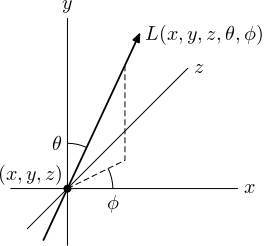
\includegraphics[width=0.5\textwidth]{./Diagrams/Plenoptic_function.jpg}
\caption{Spatio-angular parametrization of the plenoptic function for fixed $\tau$ and $\lambda$. Figure taken from Wikipedia (https://en.wikipedia.org/wiki/Light\_field)}
\end{figure}

In a more practical approach the plenoptic function can be simplified to a 4D version, called 4D Light Field or simply Light Field (abbreviated from now on as LF), denoted as the function $L$. The LF quantifies the intensity of static and monochromatic light rays propagating in half space, though this seems like an important reduction of information, this constraint does not substantially limit us in the accurate 3D description of the scene from where the light rays come from.

 There exists three tipical forms of this 4D approximation: 
\begin{enumerate}
\item The LF rays positions are indexed by their Cartesian coordinates on two parallel planes, also called the two-plane parametrization $L(u,v,s,t)$.
\item The LF rays positions are indexed by their Cartesian coordinates on a plane and the directional angles leaving each point, $L(u,v,\phi,\theta)$.
\item Pairs of points on the surface of a sphere $L(\phi_1,\theta_1,\phi_2,\theta_2)$.
\end{enumerate}

\begin{figure}[h!]
\centering
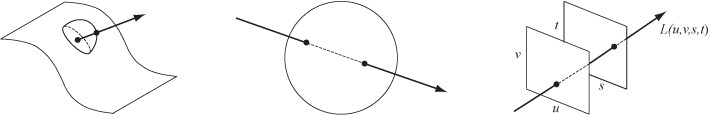
\includegraphics[width=1.0\textwidth]{./Diagrams/Light-field-parametrizations.jpg}
\caption{Three different representations of 4D LF. Left: $L(u,v,\phi,\theta)$. Center: $L(\phi_1,\theta_1,\phi_2,\theta_2)$. Right: $L(u,v,s,t)$. Figure taken from Wikipedia (https://en.wikipedia.org/wiki/Light\_field)}
\end{figure}

In this work we will centered our attention in the two plane parametrization $L(u,v,s,t)$, if you are interested in the other descriptions we recommend to see \cite{Liang}. In order to understand deeply this way of LF description, lets consider a camera with image plane coordinates $(u,v)$ and the focal distance $f$ moving along the $(s,t)$ plane. 

\begin{figure}[h!]
\centering
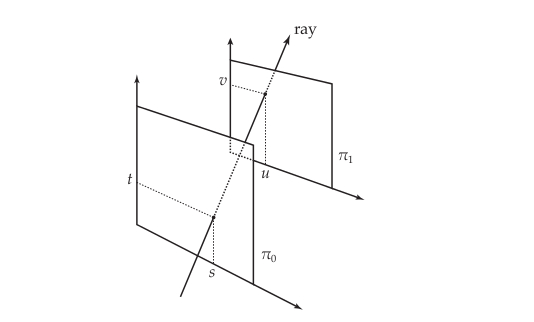
\includegraphics[width=1.0\textwidth]{./Diagrams/two-planes_param.jpg}
\caption{Graphic representation of the two plane parametrization of a single ray on the LF which is parametrized by the intersection $(s,t)$ and $(u,v)$ with planes $\pi_0$ and $\pi_1$, respectively. Figure taken from \cite{Kim-Disney} p.21}
\end{figure}

For simplicity one can constrain the vertical camera motion by fixing $s = s_0$ and moving the camera along the $t-axes$ in an straight light motion, in the section~\ref{sec:Epi-geometry} we will see that this constraint leads to an elegant geometric 3D representation of the scene called Epipolar Geometry, this multiview aquisition is refered as parallax only (HPO). Under this constraint, images captured by successive camera positions $t_1$, $t_2$,... can be stacked together, and one can also interpret each camera position as a time step.

\begin{figure}[h!]
\centering
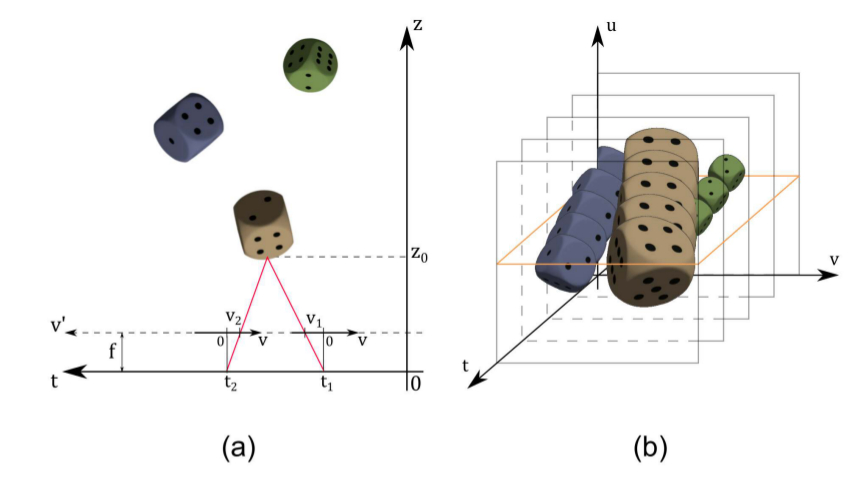
\includegraphics[width= 0.90\textwidth]{./Diagrams/images_stacked.jpg}
\caption{Stacked captured images represented in (b) from the scene setup (a). Figure taken from \cite{LF-Shearlets} p. 2}
\end{figure}

\section{Light Field Photography in the History}

For different reasons of interest for science and art capturing light fields has been an active research area for more than 110 years (the reason will be explained in detail on the section \ref{sec:LF-applications}). In 1903 Herbert E. Ives \cite{Ives} was the first to realize that the light field inside a camera can be recorded by placing a pinhole or lenslet arrays in front of a film sensor (what is know as pinhole camera). On the other hand, in 1908 the french physicist and Nobel laureate Gabriel Lippmann published two articles about something that he called \textit{photographie int\'egrale} (translated as integral photography) \cite{Lippmann} in which he describes an imaging apparatus with an arrange of small lenses on a 2D grid that are able to capture multiple images of a scene with viewpoint variations, is quite surprising that almost 110 year ago he could have the idea that modern state of the art LF aquisition systems use

\section{Epipolar Geometry, Stereo Vision and Image rectifictation}
\label{sec:Epi-geometry}

\section{Sparse aquisition of Epipolar-plane}

\section{Typical applications for the Light Field Theory}
\label{sec:LF-applications}

\chapter{Shearlets}

We want to be able to express efficiently Epipolar Plane Images that will reduce the number of minimum views needed to recover the light field of a scene; this task can be achieved by understanding the EPIs as signals and using signal processing machinery developed in the last twenty years, in this chapter we will explain in detail state-of-the-art methods on signal sparse-representation.

\bigskip

One can think a signal as a function (or something that can be represented as) that contains information about the behavior or attributes of some phenomenon \cite{Roland}, by this definition it actually could be a lot of things; it also depends the area you are working on, this definition will work or not. For example, in signal processing, arbitrary binary data streams are not considered as signals. For the sake of simplicity in this thesis we will agree to define a signal as a function that could represent video, image or audio and it will be either analog (evaluated with continuous parameters) or digital (evaluated with discrete parameters). 

\bigskip

In signal processing and applied harmonic analysis one can generally represent the signals in a space-time domain, but one cannot get always meaningful information in this representation; plenty of different signal transforms have been proposed along time, this transforms are obtained generally by finding basis of certain functional spaces (e.g. $L^2(\mathbb{R}^2)$) and present different features like sparse representation of signals that permits an efficient processing and storing of them. The most known signal transform for its effectiveness and tradition is the Fourier Transform, proposed by the French Mathematician Joseph Fourier, on his paper "Théorie analytique de la chaleur" in 1822 where he showed that some functiones could be written as an infinite sum of sines and cosines. 

\bigskip

If $f\in L^2(\mathbb{R}^n)$ then its Fourier transform $\hat{f}$ will be 
$$
\hat{f}(\xi) := \int_{\mathbb{R}^n}f(x)e^{-i\langle x,\xi\rangle}dx
$$

one can think of the coordinates $\xi$ of the Fourier space, as one can see the Fourier transform $\hat{f}$ just gives information about the frequencies contained in $f$, but not at which time they occur; moreover, small changes in the neighborhood of some point $x\in\mathbb{R}^n$ could change significantly its Fourier transform, in general one would not like that. A small solution for this issue is reflected in the short-time Fourier transform; whose mechanism is based in localization of the Fourier transform to a certain window of $f$ and then move the window through the whole domain. Let $g\in L^2(\mathbb{R})$ the window function, the short-time Fourier transform of $f\in L^2(\mathbb{R})$ associated with the window $g$ will be

$$
S_gf(t,\xi)=\int_{\mathbb{R}} f(x)\overline{g(x-t)}e^{-ix\xi}dx=\langle f,M_{\xi}T_tg\rangle = (\widehat{f\cdot T_t\overline{g}})(\xi)\text{,  } t,\xi\in\mathbb{R}
$$

where $T_t:L^2(\mathbb{R})\longrightarrow L^2(\mathbb{R})$ is the translation operator with parameter $t$, given by 
$$
T_tf(x)=f(x-t)
$$
and $M_{\xi}:L^2(\mathbb{R})\longrightarrow L^2(\mathbb{R})$ is the modulation operator, given by 
$$
M_{\xi} f(x)=e^{i\xi x}f(x)
$$

\bigskip 

One can associate to this transform the atoms $\{M_{\xi}T_tg\}_{(t,\xi)\in\mathbb{R}^2}$; for computational purposes one can discretize the transform taking $(t,\xi)\in\Lambda=a\mathbb{Z}\times b\mathbb{Z}$ for some $a,b>0$; the resulting atoms $G(g,a,b):=\{g_{am,bn}=M_{bn}T_{am}\}_{(m,n)\in\mathbb{Z}}$, for some cases of $(a,b)\in\mathbb{R}$ $G(g,a,b)$ is a generating set of $L^2(\mathbb{R})$ with an explicit recovery formula with other features, such sequence of function are known as \textbf{frames} and can be understand as the generalization of orthonormal bases, we will study them in detail on the Section~\ref{sec:ShearletsFrames}, for a further reading about Gabor frames one can check \cite{Gabor}.

\bigskip

We introduced Gabor frames to overcome some limitations of the Fourier transform; Gabor frames also present some limitations
\begin{itemize}
\item When the Gabor frame is also a orthonormal bases don't have a good time-frequency localization \cite{Gabor}.
\item The size of the window $g$ does not change so Gabor frames are not sensible to very localized information, so for instance they will never detect a singularity or regularity information of a function.
\end{itemize} 
both limitations above can be overcome using \textbf{wavelets}.

\bigskip 

The concept of wavelets and the signal transform related was introduced first time 
in 1980s by the french mathematicians Morlet and Grossmann to refer to "small wave" (or \textit{ondelette} in french) when they were studying siesimic waves (check the original paper \cite{Grossman}). The \textit{continuous wavelet transform} of a function $f\in L^2(\mathbb{R})$ associated to a mother function $\psi\in L^2(\mathbb{R})$ is defined by 

$$
\begin{aligned}
\mathcal{W}_{\psi}f(a,b)&=\int_{\mathbb{R}}f(t)a^{-\frac{1}{2}}\overline{\psi\left(\frac{t-b}{a}\right)}dt\\
&=\langle f, T_bD_a\psi\rangle = (f\ast D_a\overline{\psi}^*)(b)\text{, } (a, b)\in\mathbb{R}^+\times\mathbb{R} 
\end{aligned}
$$

where $D_a:L^2(\mathbb{R}\longrightarrow L^2(\mathbb{R})$ is the dilation operator given by $D_a f(t)=a^{-\frac{1}{2}}f\left(\frac{t}{a}\right)$, and $f^*(t)=f(-t)$, $a$ is the scaling paramter (controls the size of the window) and $b$ is the translation parameter. If the mother function $\psi$ satisfy the admissibility condition 

$$
C_{\psi}:=\int_0^{\infty}\frac{|\hat{\psi}(\xi)|^2}{\xi}d\xi <\infty
$$

we will say that $\psi$ is a admissible wavelet. If one has an admissible wavelet, one can get an straightforward inversion or recovery formula as
$$
f=\frac{1}{C_{\psi}}\int_{\mathbb{R}}\int_0^{\infty} W_{\psi}f(a,b)T_bD_a\psi\frac{da}{a^2}db
$$

\bigskip

The sequence of wavelet atoms will be $\{\psi_{a,b}(t)=a^{-\frac{1}{2}}\overline{\psi\left(\frac{t-b}{a}\right)}\}_{(a,b)\in\mathbb{R}^+}$, so one can write the wavelet transform of $f$ as $W_{\psi}f(a,b)=\langle f,\psi_{a,b}\rangle$. One can discretize the wavelet transforms as by the inner product with the discrete set of wavelet atoms
$$
\psi_{j,m}(t):=a^{-\frac{1}{2}}\psi(a^{-j}t-bm)\text{,  } (j,m)\in\mathbb{Z}^2\text{,  } t\in \mathbb{R}\text{,   }(a,b)\in\mathbb{R}^+\times\mathbb{R}
$$

the set of discrete set of wavelet atoms is referred as wavelet system. Wavelets are very relevant in Signal Processing due their great features 
\begin{itemize}
\item One can get information about the regularity of a function $f$ by estimating bounds of its wavelet transform.
\item The scaling parameter permits us to detect very localized information, in particular is very effective detecting one dimensional singularities, this property leads to the construction of a Multiresolution Analysis (MRA) which is an important area in applied harmonic analysis(check \cite{Mallat} p. 264).
\item The unified treatment of both digital and continuous transforms permits an easy implementation.
\item It can represent sparsely one dimensional signals, in the sense that not a lot of coefficients will be significant so one can  them.
\end{itemize}

\bigskip

Over all the features that we just mentioned the one that gave most of its fame to the wavelet transform is the last one, i.e.\ sparse representation of one dimensional signals, for instance this porperty of wavelets is what the image compression standard JPEG 2000 is based on. It is worth it to study in more detail sparse representation of data.

\bigskip

It is not surprising that compression of data takes an important place in the academic research and industrial agenda nowadays. Our society generates and acquire a lot of data everyday that comes in a lot of different types and dimensions; the complexity of the processing of this raw data to extract some useful data in an understandable language grows with the dimensionality and size of the data. Even though, almost all data found in practical applications has the property that the relevant information which needs to be extracted or identified is sparse, that is, data are typically highly correlated and the essential information lives in lower dimensional subspaces (or manifolds). This information can be then captured using just few terms in an appropriate dictionary (e.g.\ some frame or orthonormal basis). 

\bigskip

The sparse representation property of data is important not only for data storage and transmission but also for feature extraction, classification, and other high-level tasks; finding a dictionary which sparsely represents a certain data class involves deep understanding of its dominant properties, which are typically associated with their geometric properties; for a deep treatment of this one can read \cite{IntroShearlets} and \cite{Gitta-Lim}.

\bigskip

So far we have just mentioned the sparse representation property for one-dimensional signals and also the existence of straight forward and fast algorithmic implementations; the latter is based in the general machinery to construct orthonormal wavelet bases known as \textit{Multiresolution Analysis} (MRA). In the one dimensional case, this is defined as a sequence of closed subspaces $(V_j)_{j\in\mathbb{Z}}$ in $L^2(\mathbb{R})$ known as the scaling spaces which satisfies the following properties

\begin{enumerate}
\item[(a)] $\{0\}\subseteq\ldots\subset V_{-2}\subset V_{-1}\subset V_0\subset V_1\subset V_2\subset\ldots L^2(\mathbb{R})$.
\item[(b)] $\cap_{j\in\mathbb{Z}}V_j=\{0\}$ and $\overline{\cup_{j\in\mathbb{Z}V_j}}=L^2(\mathbb{R})$.
\item[(c)] $f\in V_j$ if and only if $D_2^{-1}f\in V_{j+1}$.
\item[(d)] There exists a $\varphi\in L^2(\mathbb{R})$, called \textit{scaling function}, such that $\{T_m\varphi:m\in\mathbb{Z}\}$ is an orthonormal basis for $V_0$.
\end{enumerate}

This enables the decomposition of functions into different "resolution" levels associated with the so called wavelet spaces $W_j$, $j\in\mathbb{Z}$ which are defined by considering the orthogonal complements
$$
W_j:= V_{j+1}\ominus V_j\text{,  } j\in\mathbb{Z}
$$

This Multiresolution Analysis let us not only to decompose $L^2(\mathbb{R})$ as a direct sum of wavelet spaces but also gives us an alternative orthonormal basis with both the wavelet and the scaling fuction, of the form

$$
\{\varphi_m=T_m\varphi=\varphi(\cdot-m):m\in\mathbb{Z}\}\cup\{\psi_{j,m}:j\geq 0,m\in\mathbb{Z}\}
$$

where the scaling function take care of the low-frequency region $V_0$ and the wavelet terms of the complementary space $L^2(\mathbb{R})\ominus V_0$. One can read \cite{Mallat}. 

\bigskip

In this thesis we are interested in image processing, if one would like to apply wavelets to imaging science an extension of the theory to $L^2(\mathbb{R}^2)$. For a painless extension we can introduce the concept of tensor products of Hilbert spaces. If $\mathcal{H}_1$ and $\mathcal{H}_2$ are two Hilbert spaces the tensor product is a bilinear operator $\otimes:\mathcal{H}_1\times\mathcal{H}_2\longrightarrow \mathcal{H}_1\otimes\mathcal{H}_2$ where $\mathcal{H}_1\otimes\mathcal{H}_2$ is a new Hilbert space.

\bigskip

We can use strongly the fact that the tensor product of orthonormal bases is an orthonormal basis of $\mathcal{H}_1\otimes\mathcal{H}_2$. In the case of $\mathcal{H}_1=\mathcal{H}_2=L^2(\mathbb{R})$ and $f,g\in L^2(\mathcal{R})$,

$$
(f\otimes g)(x_1,x_2)=f(x_1)g(x_2)\text{,  } (x_1,x_2)\in\mathbb{R}^2,
$$

and $\mathcal{H}_1\otimes\mathcal{H}_2=L^2(\mathbb{R}^2)$. This concepts leads to the next theorem.

\bigskip

\begin{thm}[Two-dimensional wavelets]
Let $(V_j)_{j\in\mathbb{Z}}$ be an MRA for $L^2(\mathbb{R})$ with scaling function $\varphi\in L^2(\mathbb{R})$ and associated wavelet $\psi\in L^2(\mathbb{R})$. For $(x_1,x_2)\in\mathbb{R}^2$, we define
$$
\begin{aligned}
&\psi^1(x_1,x_2):=\varphi(x_1)\psi(x_2),\\
&\psi^2(x_1,x_2):=\psi(x_1)\varphi(x_2),\\
&\psi^3(x_1,x_2):=\psi(x_1)\psi_(x_2)
\end{aligned}
$$
Then 
$$
\{\psi_{j,m}^k(x_1,x_2)=2^{-j}\psi^k(2^{-j}x_1-m_1,2^{-j}x_2-m_2)\text{: } m=(m_1,m_2)\in\mathbb{Z}^2,k=1,2,3\}
$$
is an orthonormal basis for the wavelet space $W^2_j$, given by $V^2_j\oplus W^2_j=V^2_{j-1}$. Moreover,
$$
\{\psi_{j,m}^k\text{:  }j\in\mathbb{Z},m=(m_1,m_2)\in\mathbb{Z}^2,k=1,2,3\}
$$
is an orthonormal basis for $L^2(\mathbb{R}^2)$.
\end{thm}
\begin{proof}
One can find the proof on \cite{Mallat}, pp. 340-346.
\end{proof}

\bigskip

There exists more general non-separable two dimensional wavelets transforms using the continuous affine group to generalize the dilation operator $D_a$ to $D_M$ for two-dimensional invertible matrices $M$. The traditional theory of wavelets is based on the use of isotropic dilations and therefore is esentially a one-dimensional theory, so it is unable to give additional information about the geometry of the set of singularities of a function or distribution that are multivariate. The main problem is that the isotropic wavelet transform is simple but lacks of directional sensitivity and the ability to detect the multidimensional geometry of a function or distribution $f$.

\bigskip

One can formalize this notion using the concept of best $N$-term approximation. We will provide the general definition applied to dictionaries (collection of vectors on a Hilbert space $\{\varphi_i: i\in I\}\subseteq \mathcal{H}$ with $I$ finite or countable infinite).

\bigskip

\begin{defn}[Best N-term Approximation]
Let $D:=\{\varphi_i\text{:  }i\in I\}\subseteq \mathcal{H}$ be a dictionary. Consider a vector $x\in\mathcal{H}$ and an integer $N\in\mathbb{N}$. Then the \textit{best N-term approximation of x} with respect to $D$ is defined by the solution of the following minimization problem:
$$
\min_{I_N,(c_i)_{i\in I_N}}||x-\sum_{i\in I_N} c_i\varphi_i|| \text{ subject to } I:N\subseteq I,\# I_N\leq N
$$
\end{defn}

\bigskip

The best N-term approximation $f_N$ of $f\in L^2(\mathbb{R}^2)$ with respect to the dictionary formed by the wavelet basis can be understan as the obtained by approximating $f$ from its $N$ largest wavelet coefficients in magnitude. Let $\Lambda_N$ the index set corresponding to the $N$- largest wavelet coefficients $|\langle f,\psi_{\lambda}\rangle|$ associated with some wavelet basis $(\psi)_{\lambda\in\Lambda}$, the best $N$-term approximation will be
$$
f_N=\sum_{\lambda\in\Lambda_N}\langle f,\psi_{\lambda}\rangle\psi_{\lambda}
$$

\bigskip

To study the approximation of natural images by the wavelets, we first need to introduce a definition of what we will understand mathematically as a natural image, the so called \textit{cartoon-like functions}.

\bigskip

\begin{defn}[Cartoon-like functions]
The class of \textit{cartoon-like functions} $\mathcal{E}^2(\mathbb{R}^2)$ is defined as the set of functions $f:\mathbb{R}^2\longrightarrow \mathbb{C}$ of the form $f= f_0+\chi_B f_1$. Here, we assume that $B\subseteq [0,1]^2$ where $\partial B\in C^2$ and bounded curvature. Moreover, $f_i\in C^2(\mathbb{R}^2)$ with $||f_i||_{C^2}\leq 1$ and $\text{supp} f_i\subset [0,1]^2$ for $i=0,1$. 
\end{defn}

\bigskip

\begin{figure}[h!]
\centering
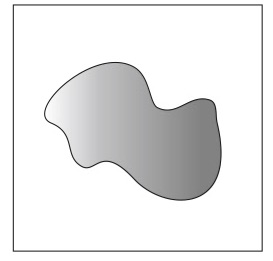
\includegraphics[width = 0.4 \textwidth]{./Diagrams/cartoon-like.jpg}
\caption{Example of a cartoon-like image. Figure taken from \cite{IntroShearlets} pp. 9}
\label{fig:cartoon-like}
\end{figure}

Now, let $f$ be a cartoon-like image containing a singularity along a smooth curve and $\{\psi_{j,m}\}$ be a standard wavelet bases of $L^2(\mathbb{R}^2)$. For $j$ sufficiently large, the only significan wavelet coefficients $\langle f,\psi_{ j,m}\rangle$ are the ones associated with the singularity. At each scale $2^{-j}$, each wavelet $\psi_{j,m}$ is supported inside a box of size $2^{-j}\times 2^{-j}$, there exist about $2^j$ elements of the wavelet basis overlapping the singularity curve. The associated wavelet coefficients are controlled by 

$$
|\langle f,	\psi_{j,m}\rangle|\leq ||f||_{\infty}||\psi_{j,n}||_{L^1(\mathbb{R}^2)}\lesssim 2^{-j}
$$

It follows that the $N$-th largest wavelet coefficient in magnitude, denoted by $\langle f,\psi_{j,m}\rangle_{(N)}$, is bounded by O($N^{-1}$). Thus, if $f$ is approximated by its best $N$-term approximation $f_N$, the $L^2$ error (called  best $N$-term approximation error) obeys

$$
\sigma_N(f,\{\psi_{j,m}\}_{j,m}^2=||f-f_N||^2_{L^2(\mathbb{R}^2)}\leq \sum_{\ell\geq N}|\langle f,\psi_{j,m}\rangle_{(l)}|^2\lesssim N^{-1}
$$

This estimate is actually tight, in the sense that there exist cartoon-like images for which the best $N$-term approximation error is

$$
\sigma_N(f,\{\psi_{j,m}\}_{j,m})\approx N^{-\frac{1}{2}}
$$
the proof of this result can be founded in \cite{Mallat}.

Even this looks like a nice result, it is far from optimal.

\bigskip

\begin{thm}
\label{C3S2T1}
Let $\{\psi_{\lambda}\}_{\lambda\in\Lambda}\subseteq L^2(\mathbb{R}^2)$ be a frame for $L^2(\mathbb{R}^2)$. Then the optimal best $N$-term approximation error for any $f\in\mathcal{E}^2(\mathbb{R}^2)$ is
$$
\sigma_N(f,\{\psi_{\lambda}\}_{\lambda\in\Lambda})=O(N^{-1})
$$
\end{thm}
\begin{proof}
In Section~\ref{sec:ShearletsFrames} we will define the concept of frame. This result was proved by Donoho in 2001 on \cite{DonohobestNterm}, so one can refer to his proof.
\end{proof}

\bigskip

As we mentioned before, the problem with wavelets that does not make them to approach efficiently multivariate data is related to its isotropic scaling characteristic that makes them not sensible to directions. The question that can arise is, "Why should we care about anisotropic features related to multidimensional singularities?"; all the multivariate data are typically dominated by anisotropic features such as singularities on lower dimensional embedded manifolds; for example by edges in natural images or shock fronts in the solutions of transport equations. 

\begin{figure}[h!]
\centering
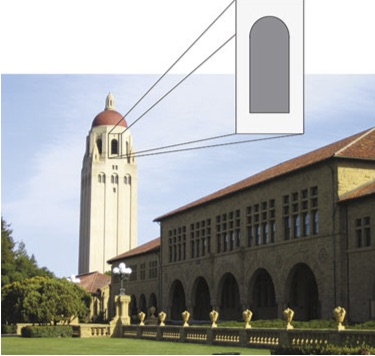
\includegraphics[width = 0.7\textwidth]{./Diagrams/edges-images.jpg}
\caption{Natural images governed by anisotropic structures. Figure taken from \cite{IntroShearlets} pp. 8}
\label{edges-images}
\end{figure}

\bigskip

The bound result of theorem~\ref{C3S2T1} works as a benchmark for optimally sparse approximation of two-dimensional data in form of cartoon-like functions. Moreover, to proof theorem~\ref{C3S2T1} Donoho used adapted triangulations, which suggests that analyzing elemnts with elongated and orientable supports are required to get optimally sparse approximations of piecewise smooth two-dimensional functions. This observation leaded to two different approaches for solving this problem, the curvelets (proposed by E. Candès and D. Donoho in 1999 \cite{Curvelets}), and the shearlets (proposed by Kanghui Guro, Gitta Kutyniok and Demetrio Labate in 2005 \cite{FirstShearlets}), both are able to achieve the same optimal approximation rate; the one used in this thesis to sparsely represent EPIs is the latter due the possibility to develope a faithful implementation. 

\section{Shearlet Systems and Transform}
\label{sec:shearletsystem}

We just discussed the limitations of wavelet systems in higher dimensions, we will then the concept of shearlet systems as a framework to solve these limitations. We also mentioned that in order to achieve optimally sparse approximations of signals with anisotropic singularities such as cartoon-like images, the analyzing elements must be made by waveforms ranging over several scales, orientations, and locations with the ability to become very elongated. One need then the combination of an appropriate scaling operator to generate elements at different scales, an orthogonal operator to change their orientations, and a translation operator to displace the elements over the two-dimensional plane. 

\bigskip

By tradition and effectivenes one can use the family of dilation operators $D_{A_a}$, $a>0$ based on parabolic scaling matrices $A_a$ of the form

\begin{equation}
\label{eq:scaling}
A_a:=
\left(
\begin{matrix}
a & 0 \\
0 & a^{1/2}
\end{matrix}
\right)
\end{equation}

This is the first approach to a scaling operator by the long history of parabolic scaling in harmonic analysis literature \cite{Fefferman}; the so called \textit{Classical Shearlets} use this approach, one can generalize the scaling using matrices of the form 

\begin{equation}
\label{eq:scalingalpha}
A_a:=
\left(
\begin{matrix}
a & 0 \\
0 & a^{\alpha/2}
\end{matrix}
\right)
\end{equation}

with $\alpha\in (0,2)$ that controls the "degree of anisotropy" and the generated system is known as \textit{Alpha Shearlets}, we will discuss this in detail on Section~\ref{sec:AlphaShearlets}. Parabolic scaling is also knwon to be required in order to obtain optimally sparse approximations of cartoon-like images, since it is the best adapted to $C^2$-regularity of the curves of discontinuity, i.e.\ is efficient to approximate smooth curves, moreover choosing $a=2$ gives the best performance.

\bigskip

 Next, we need an orthogonal transformation to change to change the orientation of the waveforms. One does not use rotations since it destroys the structure of the integer lattice $\mathbb{Z}^2$ whenever the rotation angle is different from $0,\pm\frac{\pi}{2},\pm\frac{3\pi}{2}$, which will represent an issue in the discrete setting. One chooses the shearing operator $D_s$, $s\in\mathbb{R}$, where the \textit{shearing matrix} $S_s$ is given by 
\begin{equation}
\label{eq:shearing}
S_s=
\left(
\begin{matrix}
1 & s \\
0 & 1
\end{matrix}
\right)
\end{equation}

with this two elements we are ready to define the Continuous Shearlet Transform.

\begin{figure}[h!]
\centering
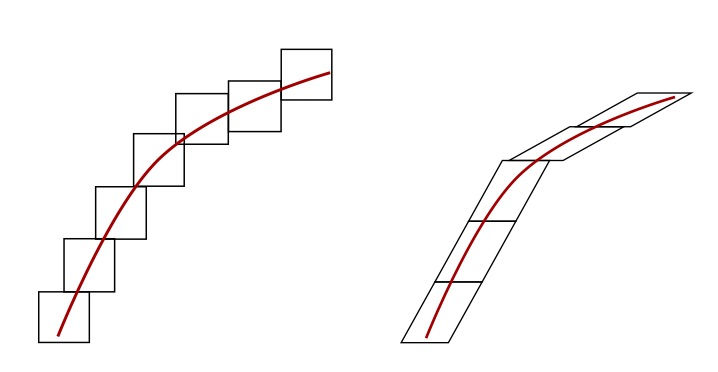
\includegraphics[width = 0.7\textwidth]{./Diagrams/anisotropic_isotropic.jpg}
\caption{Optimal covering of anisotropic scaled and sheared atoms}
\label{edges-images}
\end{figure}

\begin{figure}[!tbp]
  \centering
  \begin{minipage}[b]{0.45\textwidth}
    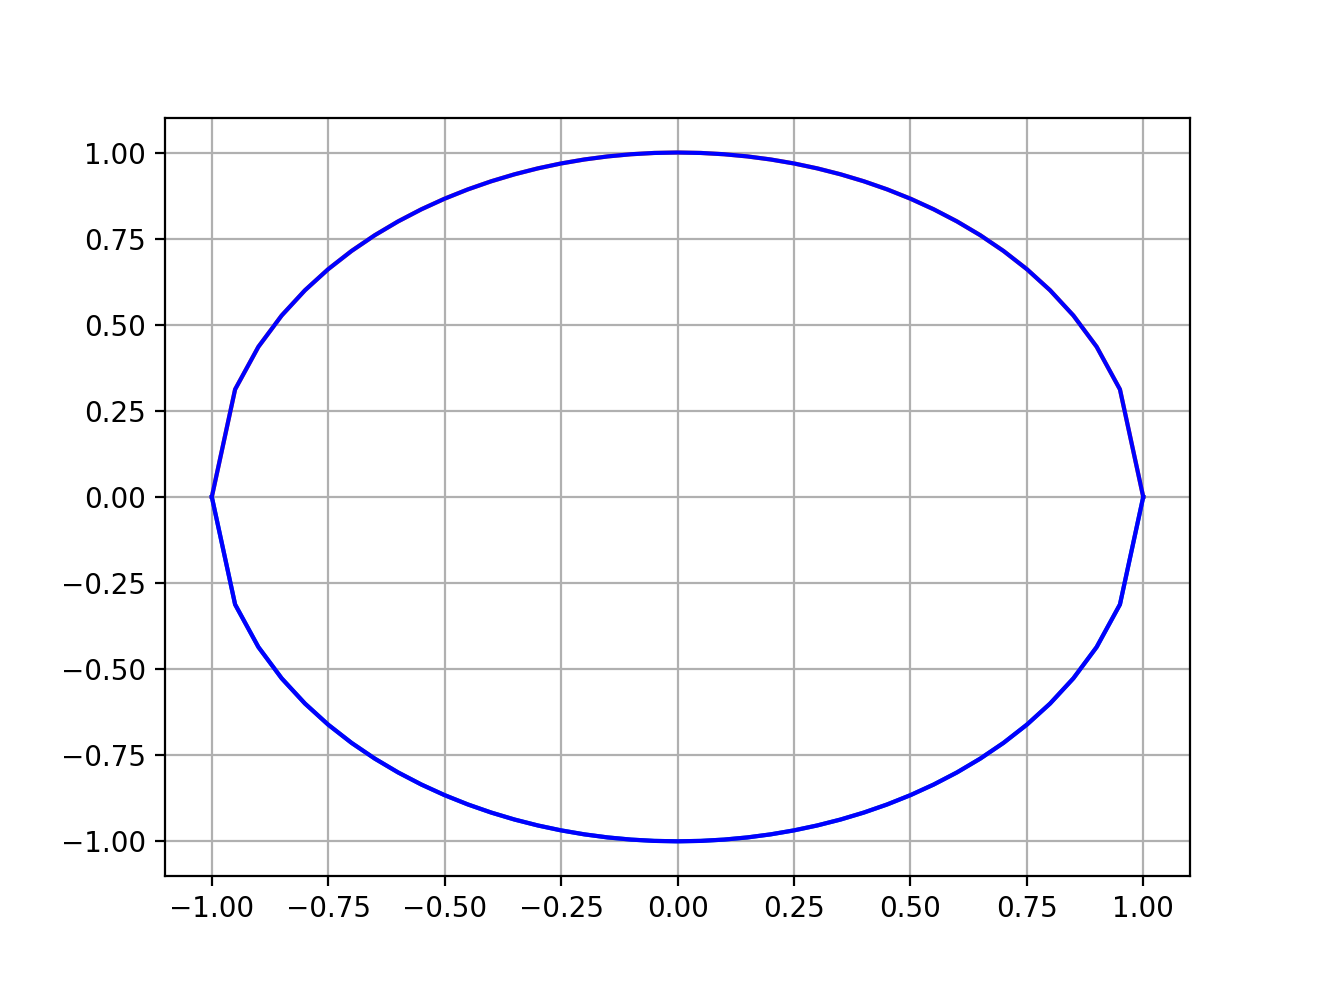
\includegraphics[width=\textwidth]{./Diagrams/circle.png}
    \caption{Circle before parabolic scaling}
  \end{minipage}
  \hfill
  \begin{minipage}[b]{0.45\textwidth}
    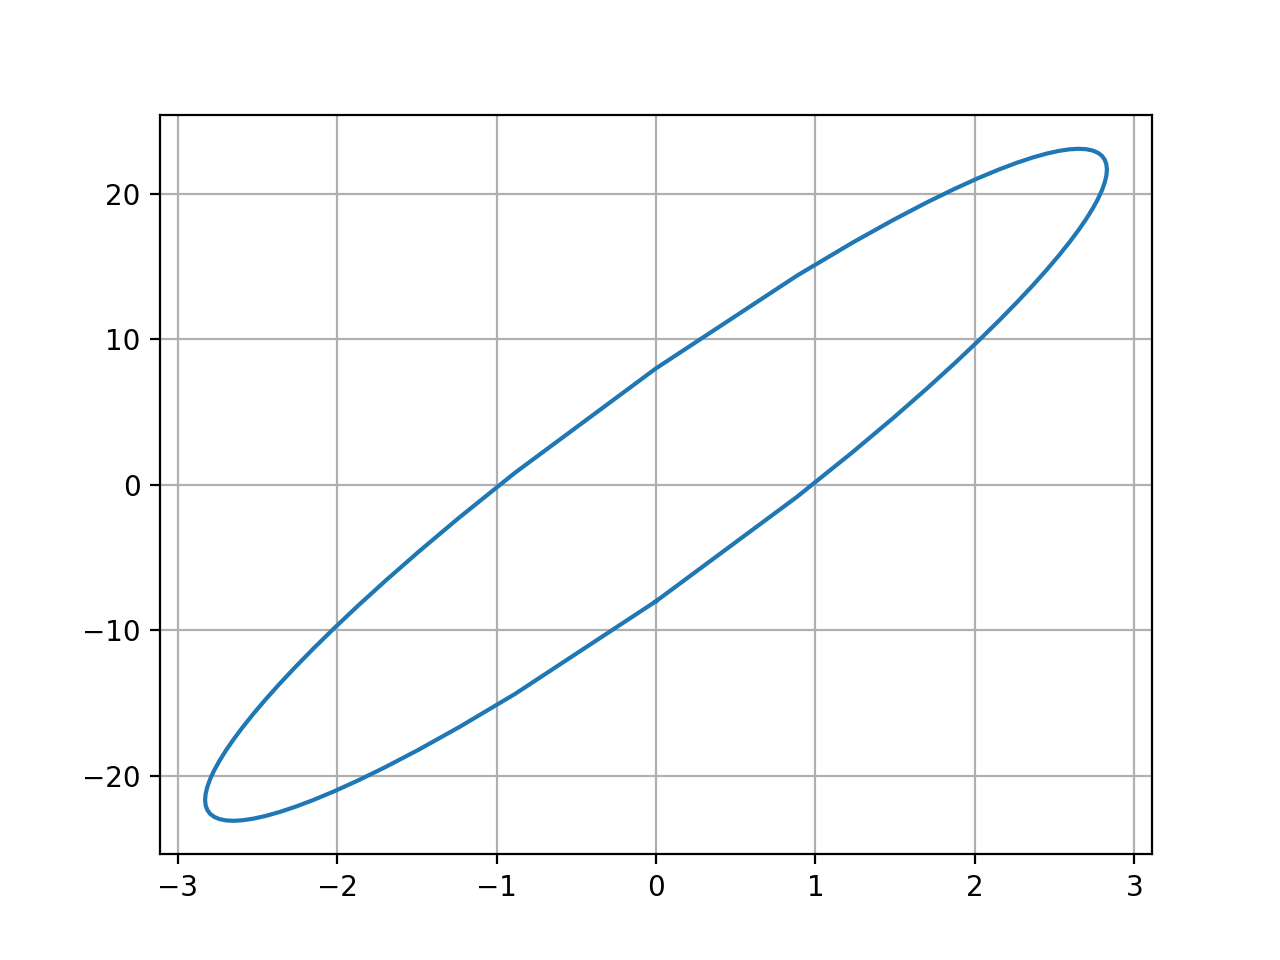
\includegraphics[width=\textwidth]{./Diagrams/circle_scaled.png}
    \caption{Circle after parabolic scaling $a=4$}
  \end{minipage}
\end{figure}


\begin{figure}[!tbp]
  \centering
  \begin{minipage}[b]{0.45\textwidth}
    
\includegraphics[width=\textwidth]{./Diagrams/square.png}
    \caption{Square before shearing}
  \end{minipage}
  \hfill
  \begin{minipage}[b]{0.45\textwidth}
    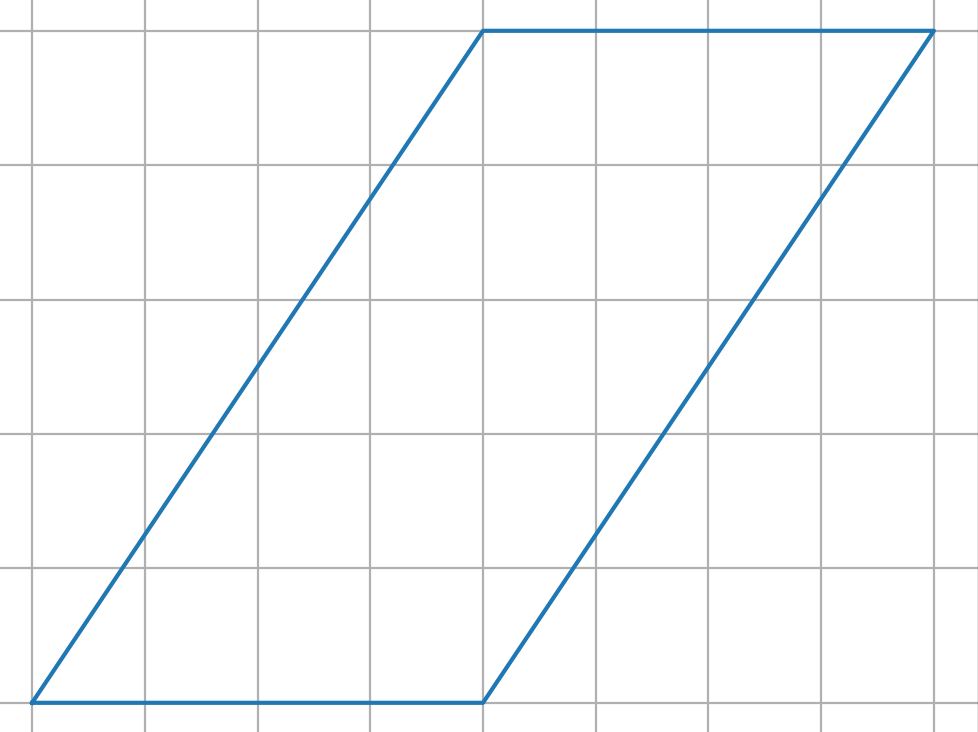
\includegraphics[width=\textwidth]{./Diagrams/square_sheared.png}
    \caption{Sheared square by a factor of $k=1$}
  \end{minipage}
\end{figure}


\begin{defn}[Continuous Shearlet Transform]
Let $\psi\in L^2(\mathbb{R}^2)$, $A_a$ and $S_s$ the parabolic scaling matrix and shearing matrix defined in~\ref{eq:scaling} and~\ref{eq:shearing} respectively, then the continuous shearlet system $SH(\psi)$ associated with $\psi$ is defined by
\begin{equation}
\label{eq:contshearletsys}
\mathcal{SH}(\psi):=\{\psi_{a,s,t}=a^{1/2}\psi (S_sA_ax-t):a\in\mathbb{R}^+,s\in\mathbb{R},t\in\mathbb{R}^2\}
\end{equation}
\end{defn}

In analogy with the discretization of wavelets, one can discretize faithfully the shearlet system which permits a straight forward implementation. We will use $a=2$ for scaling parameter since it was proven to be the best choice.

\begin{defn}[Discrete Shearlet Transform]
Let $\psi\in L^2(\mathbb{R}^2)$, $j\in\mathbb{Z}$, lets define the \textit{discrete parabolic scaling matrix} as follows

\begin{equation}
\label{eq:discscaling}
A_j:= A_2^j =
\left(\begin{matrix}
2^j & 0 \\
0 & 2^{j/2}
\end{matrix}\right)
\end{equation}

and the \textit{discrete shearing matrix} for $k\in\mathbb{Z}$

\begin{equation}
\label{eq:discshearing}
S_k:= 
\left(\begin{matrix}
1 & k \\
0 & 1
\end{matrix}\right) 
\end{equation}

Given $\psi\in L^2(\mathbb{R}^2)$, the discrete shearlet system associated with $\psi$ is defined as

\begin{equation}
\label{eq:discshearletsys}
\mathcal{DSH}(\psi):=\{\psi_{j,k,m}(x)=2^{3j/4}\psi (S_kA_jx-m):j\in\mathbb{Z},k\in\mathbb{Z},m\in\mathbb{Z}^2\}
\end{equation}
\end{defn}

It has been proved that Shearlets present a lot of features and breakthrough results; for instance they can perform common tasks of signal processing as inpainting or denoising with great results in comparison with other methods (e.g.\ wavelets); but we defined the Shearlet System with motivation on the optimal best $N$-term approximation error found by Donoho (see Theorem~\ref{C3S2T1}), and prove that this bound is reached one first need to give some definitons.

\begin{defn}[Classical shearlets]
\label{def:classical_shearlets}
Let $\psi\in L^2(\mathbb{R}^2)$ be defined by
$$
\hat{\psi}(\xi_1,\xi_2)=\hat{\psi}_1(\xi_1)\hat{\psi}_2\left(\frac{\xi_2}{\xi_1}\right)
$$
where $\psi_1,\psi_2\in L^2(\mathbb{R})$ satisfy the following properties:
\begin{itemize}
\item $\sum_{j\in\mathbb{Z}} |\hat{\psi}_1(2^{-j}\xi)|^2=1$ for a.e. $\xi\in\mathbb{R}$ (\textit{wavelet like}).
\item $\text{supp}(\hat{\psi}_1)\subseteq \left[ \frac{1}{2},-\frac{1}{16}\right]\cup\left[\frac{1}{16},\frac{1}{2}\right]$
\item $\hat{\psi}_1\in C^{\infty}(\mathbb{R})$.
\item $\sum_{k=-1,0,1}|\hat{\psi}_2(\xi+k)|^2=1$ for a.e. $\xi\in [-1,1]$ ("bump-like").
\item $\text{supp}(\hat{\psi}_2)\subseteq [-1,1]$.
\item $\hat{\psi}_2\in C^{\infty}(\mathbb{R})$.
\end{itemize}
Then, we call $\psi$ a \textit{classical shearlet}.
\end{defn}

\begin{figure}[!tbp]
  \centering
   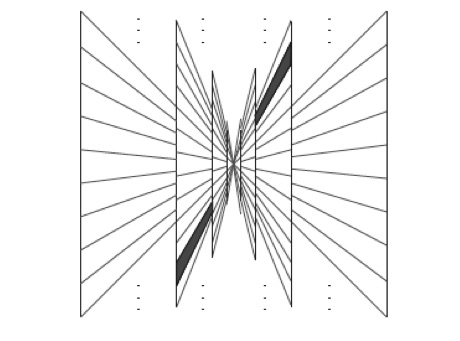
\includegraphics[width=0.7\textwidth]{./Diagrams/tiling_nocone.jpg}
    \caption{Tiling of the Fourier domain for the classical shearlets. Figure taken from \cite{Gitta-notes}, pp. 82}
  \label{fig:tiling_nocone}

\end{figure}

One can observe in  the tiling of the Fourier domain of the classical shearlets in Figure~\ref{fig:tiling_nocone} that the tiling of the Fourier domain of the classical shearlets is not uniform at all, it is very biased towards the $\xi_2$-axis, that will lead to some issues if one wants to analyze singularities aligned with the $x_1$-axis. For directional systems as the shearlet system one would like to have a uniform tiling of the Fourier space; to achieve this one can split the space in "cones" and associate different shearlet system for each cone. 

\bigskip

\begin{defn}[Cone-adapted shearlet system]
\label{def:cone_shearlets}
Let $\phi,\psi,\tilde{\psi}\in L^2(\mathbb{R}^2)$ and $c=(c_1,c_2)\in (\mathbb{R}^+)^2$. The \textit{cone-adapted shearlet system} associated with $\phi,\psi,\tilde{\psi}$ and $c$ is defined by 
$$
\mathcal{SH}(\phi,\psi,\tilde{\psi},c):=\Phi(\phi,c_1)\cup\Psi(\psi,c)\cup \tilde{\Psi}(\tilde{\psi},c)
$$

where

$$
\begin{aligned}
\Phi(\phi,c_1)&:=\{\phi(x-c_1m)\text{: }m\in\mathbb{Z}\},\\
\Psi(\psi,c)&:=\{2^{3j/4}\psi(S_kA_jx-M_cm)\text{: } j\geq 0,|k|\leq\lceil 2^{j/2}\rceil,m\in\mathbb{Z}^2\},\\
\tilde{\Psi}(\tilde{\psi},c)&:=\{2^{3j/4}\tilde{\psi}(\tilde{S}_k\tilde{A}_jx-\tilde{M}_cm)\text{: } j \geq 0,|k|\leq\lceil 2^{j/2}\rceil,m\in\mathbb{Z}^2\},
\end{aligned}
$$

with 

$$
M_c=\left(\begin{matrix} c_1 & 0 \\ 0 & c_2\end{matrix}\right)\text{,  }
\tilde{M}_c=\left(\begin{matrix} c_2 & 0 \\ 0 & c_1\end{matrix}\right) \text{,  }
\tilde{S}_k=\left(\begin{matrix} 1 & 0 \\ k & 1 \end{matrix}\right)\text{,  }
\tilde{A}_j=\left(\begin{matrix} 2^{j/2} & 0 \\ 0 & 2^j\end{matrix}\right)
$$

Lets split the Fourier space in cones $\mathcal{C}_1, \mathcal{C}_2, \mathcal{C}_3,\mathcal{C}_4$ and a central low-frequency square $\mathcal{R}$, see Figure~\ref{fig:tiling_cone}. Then the set

$$
\mathcal{P}_{\mathcal{R}}\Phi(\phi,1)\cup \mathcal{P}_{\mathcal{C}_1}\Psi(\psi,(1,1))\cup\mathcal{P}_{\mathcal{C}_2}\tilde{\Psi}(\tilde{\psi},(1,1))
$$

where 
$$
\begin{aligned}
\mathcal{C}_1\cup \mathcal{C}_3 &:=\mathcal{C}_h =\{ (\xi_2,\xi_1)\in\mathbb{R}^2| |\xi_2/\xi_1|\leq 1,|\xi_1|>1\}\\
\mathcal{C}_2\cup \mathcal{C}_4 &:= \mathcal{C}_v =\{ (\xi_1,\xi_2)\in\mathbb{R}^2||\xi_2/\xi_1|> 1, |\xi_2|>1\},\\
\mathcal{R}&:=\{ (\xi_1,\xi_2)\in\mathbb{R}^2||\xi_1|,|\xi_2|\leq 1\}
\end{aligned}
$$
and $P_{\mathcal{R}}$, $\mathcal{P}_{\mathcal{C}_1}$ and $\mathcal{P}_{\mathcal{C}_2}$ are the projections in the Fourier domain, is called the \textit{Cone-adapted shearlet transform}.
\end{defn}

\begin{figure}[!tbp]
  \centering
   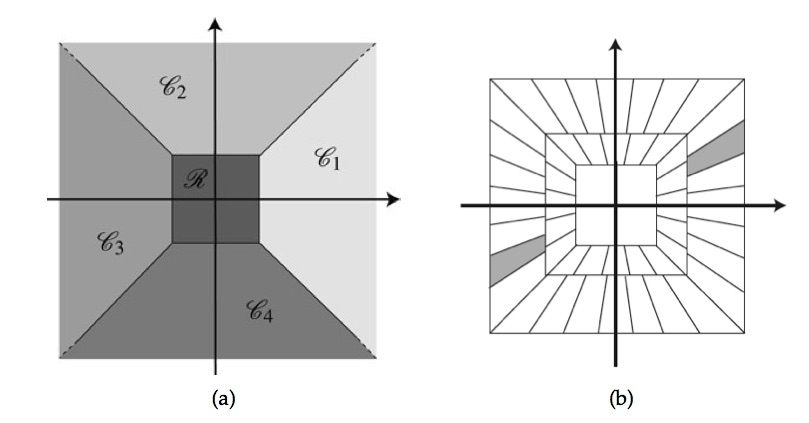
\includegraphics[width=0.9\textwidth]{./Diagrams/tiling_cone.jpg}
    \caption{(a) Tiling of the Fourier domain into cones. (b) Frequency tiling generated by cone-adapted shearlets. Figure taken from \cite{Gitta-notes} pp. 83 }
  \label{fig:tiling_cone}
\end{figure}

\bigskip

In the case of the wavelet transform the discretization and implementation of the algorithm that performs it since dilation can be performed by subsampling and one can use fourier transform properties to translate convolution into multiplication and that can be implemented optimally with the fft-algorithm. Once can also take in account that the convolution operation with a function of compact support can be thought as a filtering operation in signal processing, so a wavelet system and a multeresolution analysis  is interpreted in typical implemenation as a filter bank, the last using a high pass and a low pass filter that characterize the interaction of the wavelet and scaling function, the former obeying the admissibility condition. 

\bigskip

The Shearlet Transform of a function $f\in L^2(\mathbb{R}^2)$, $\langle f,\psi_{j,k,m}\rangle$ for the same reasons has a faithfull implementation using filtering and subsampling operations just taking care of the invariance of the $\mathbb{Z}^2$ grid under the discretization of the shearlet operator (Wang-Q. Lim proposed a solution for this on \cite{Nonseparableshear}); the filters need to characterize the functions $\phi$ and $\psi$ on the cone-adapated shearlet system (Definition~\ref{def:cone_shearlets}). The simplest choice is to take $\psi$ to be the tensor product of a wavelet function $\psi_1$ and a scaling function $\phi_1$ related to a multiresolution analysis, this approach is known as the separable shearlet generator. 

$$
\begin{aligned}
\phi(x_1,x_2)&=\phi_1(x_1)\phi_1(x_2)\\
\psi(x_1,x_2)&=\psi_1(x_1)\phi_1(x_2)
\end{aligned}
$$

Even this separable approach forms a frame a frame for $L^2(\mathbb{R}^2)$ (check Section~\ref{sec:ShearletsFrames} for a detail explanation) and simplifies the implementation, it is not a good choice for directional representations; the separability causes a significant overlap between $\text{supp}(\hat{\psi}_{j,k,m})$ and $\text{supp}(\hat{\psi}_{j,k+1,m})$, see Figure~\ref{fig:separable_nonseparable}. Also in Figure~\ref{fig:separable_nonseparable} one can see that wedge shaped support is well adapted for covering the frequency domain by the application of the shear and scale operator while improving directional selectivity to achieve this Wang-Q. Lim proposed in 2013 a non-separable shearlet generator $\psi^{\text{non}}$ given by the relation

$$
\hat{\psi}^{\text{non}}(\xi)=P\left(\frac{\xi_1}{2},\xi_2\right)\hat{\psi}(\xi),
$$

where $\psi$ is the already mentioned separable shearlet generator and $P$ is a 2D directional fan filter (see \cite{Nonseparableshear} for a more detailed explanation of this filter). The wedge form that non-separable shearlet generators give to the shearlet system the ability to cover the Fourier domain optimally. We will use this approach in this thesis; the implementation of the non-separable shearlet transform is widely explained in \cite{Shearlab} where the most known implemenation is based on, Shearlab3D in matlab (one can download it in \url{shearlab.org}); by the improvement of performance we will use the Julia Programming Language (\url{https://julialang.org/}) implementation of this library that can be downloaded in \url{https://github.com/arsenal9971/Shearlab.jl} or installed from the Julia REPL using \lstinline[language=julia]{Pkg.add("Shearlab")}.

\begin{figure}[h!]
\centering
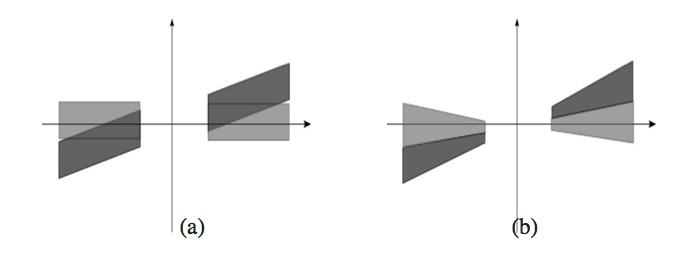
\includegraphics[width=0.8\textwidth]{./Diagrams/separable_nonseparable.jpg}
\caption{Frequency covering by shearlets $\psi_{j,0,m}$ and $\psi_{j,1,m}$ (a) with separable generator (b) with non-separable generator. Figure taken from \cite{Nonseparableshear} pp. 12}
\label{fig:separable_nonseparable}
\end{figure}

We finally can give in this section the result that we were looking for to justify formally the superiority of the Shearlet System over the Wavelet System on representating optimally the \textit{cartoon-like functions}, we will again make use of the term frame, despite it has not been introduced yet, but until the next section.

\begin{thm}
\label{thm:optimal_shearlets}
Let $\psi\in L^2(\mathbb{R}^2)$ be compactly supported.

Assume that  for $\alpha>5$, $\gamma\geq 4$, $q>q'>0$ and $q>r>0$, it holds that
\begin{equation}
\label{eq:boundframe}
|\hat{\psi}(\xi_1,\xi_2)|\leq C \min\{1,|q\xi_1|^{\alpha}\}\min\{1,|q'\xi_1|^{-\gamma}\}\min\{1,|r\xi_2|^{-\gamma}\}
\end{equation}
for some constant $C>0$ and that for $h\in L^1(\mathbb{R}^1)$ 
$$
|\frac{\partial}{\partial\xi_2}\hat{\psi}(\xi)|\leq |h(\xi_1)|\left(1+\big| \frac{\xi_2}{\xi_1}\big|\right)^{-\gamma}
$$
is satisfied. Assume that the same conditions are satisfied for $\tilde{\psi}$. Then, if the \textit{cone-adapated shearlet system} on definition~\ref{def:cone_shearlets} $\mathcal{SH}(\phi,\psi,\tilde{psi},(1,1))$ forms a frame for $L^2(\mathbb{R}^2)$, then there exists a constant $C'>0$ such that for all $f\in\mathcal{E}^2(\mathbb{R}^2)$, we have 

\begin{equation}
\label{eq:optimalshearlets}
\sigma_N(f,\mathcal{SH}(\phi,\psi,\tilde{\psi},(1,1))\leq C'N^{-1}(\log N)^{3/2} \text{as  } N\longrightarrow\infty
\end{equation}
\end{thm}
\begin{proof}
The proof of this theorem is quite technical and it has not a great impact on the results of our thesis, so one will let the reader to consult \cite{FirstShearlets} for a detailed proof. 
\end{proof}

As $N$ goes bigger the logarithm in the estimate~\ref{eq:optimalshearlets} can be taken as a constant, so Theorem~\ref{thm:optimal_shearlets} shows that the Cone-Adapted Shearlet System atains the theoretical optimal best $N$-term approximation error for the cartoon like functions given in Theorem~\ref{C3S2T1}. Cartoon-like functions represent accurately natural images, so this system is proven to be a great option to inpaint EPIs in this thesis. In the next sections we will show other features of the Shearlets as its character of frames for $L^2(\mathbb{R}^2)$ as well as other forms of them using general scaling matrix, called alpha shearlets and we will show why a particular case of alpha shearlets is the best to inpaint sparse-sampled EPIs.

\section{Shearlets as Frames}
\label{sec:ShearletsFrames}

Lets now take a bigger picture on representation systems. An orthonormal basis for Hilbert space $\mathcal{H}$ is a sequence $(\phi_i)_{i\in I}\subset\mathcal{H}$ such that for each vector $x\in\mathcal{H}$
\begin{equation}
\label{eq:parseval}
x=\sum_{i\in I}\langle x,\phi_i\rangle \phi_i
\end{equation}

so one can represent each vector in termos of the collection and one can decompose each element $x\in\mathcal{H}$ as
$$
x\mapsto (\langle x,\phi_i\rangle)_{i\in I}\text{,  }\mathcal{H}\longrightarrow \ell_2(I)
$$

even this two features (decomposition and recovery) are very simply expressed for orthonormal bases, one woul like to extend the theory for different reasons. For example, it is not possible to recover $x$ if one loses some of the coefficients $\langle x, \phi_i\rangle$, so the induced decomposition is not robust. In the last section we mentioned the imporance of sparse representation of signals in different applications, but an orthonormal basis forces the representation coefficients to be $\langle x,\phi_i\rangle$, the sequence of coefficients will not have a rapid decay. One will call this two mentioned characteristics as \textit{Robust Decomposition}, and \textit{Sparse representation}. 
p
\bigskip

A natural generalization of the convept of orthonormal bases is the concept of frames, to define them one weakens the Parseval equation~\ref{eq:parseval}.

\bigskip

\begin{defn}[Frames]
\label{def:frames}
\begin{enumerate}
\item[(1)] A sequence $(\phi_i)_{i\in I}$ in a Hilbert space $\mathcal{H}$ is called a \textbf{frame} for $\mathcal{H}$, if there exist constans $0<A\leq B<\infty$ such that
\begin{equation}
\label{eq:frames}
A||x||^2\leq \sum_{i\in I}|\langle x,\phi_i\rangle|^2\leq B||x||^2 \text{,  }\forall x\in \mathcal{H}
\end{equation}
$A$ and $B$ are called lower and upper frame bound.
\item[(2)] If $A$ and $B$ can be chosen to be equal, we call it ($A$-) tight frame. If $A=B=1$ is possible, $(\phi_i)_{i\in I}$ forms a Parseval frame.
\item[(3)] If only the upper bound in~\ref{eq:frames} holds, we call $(\phi_i)_{i\in I}$ a Bessel sequence.
\end{enumerate}
\end{defn}

\bigskip

With this definition an orthonormal basis will be a Parseval frame. Since $A>0$ frames also span the whole space $\mathcal{H}$, frames allows one to obtain both characteristics \textit{robust decomposition} and \textit{sparse representation}; for a detailed explanation of this we highly recommend the Chapter 5 of \cite{Mallat}.

\bigskip

In the last section we introduced different representation systems for signals in $L^2(\mathbb{R}^2)$, as Gabor systems that emerge motivated by the short time fourier transform, wavelet and shearlet systems. This systems will form a frame under certain conditions on the generating functions and parameters. For example in the case of wavelet systems we have the next theorem that gives a necessary condition to form frames.

\bigskip

\begin{thm}[Necessary condtion for wavelet wrames]
Let $a>1$, $b>0$ and $\psi\in L^2(\mathbb{R})$ a wavelet function such that the related system $W(\psi,a,b)$ forms a frame for $L^2(\mathbb{R})$ with frame bounds $A$ and $B$. Then, we have
$$
A\leq \frac{1}{b}\sum_{j\in\mathbb{Z}}|\hat{\psi}(a^j\xi)|^2\leq B \text{,   }\forall\xi\in\mathbb{R}
$$
\end{thm}
\begin{proof}
One can find the proof in Theorem 3.3 of \cite{daubechies}
\end{proof}

\bigskip

Sufficient conditions of wavelet frames are more technical and one can find them in Theorem 3.15 of \cite{Gitta-notes}. In our case we would like to know under what conditions \textit{Classical Shearlets} and \textit{Cone-adapted shearlets} separable and nonseparable form frames, and for that we have the next results.

\begin{thm}
Let $\psi$ be a classical shearlet, i.e.\ obeys the conditions~\ref{def:classical_shearlets}. Then the associated wavelet system $\mathcal{SH}(\psi)$ forms a Parseval frame for $L^2(\mathbb{R}^2)$.
\end{thm}
\begin{proof}
By the above properties of $\psi_1$ and $\psi_2$, we have
$$
\begin{aligned}
\sum_{j\in\mathbb{Z}}\sum_{k\in\mathbb{Z}}|\hat{\psi}(S^T_{-k}A_{-j}\xi)|^2&=\sum_{j\in\mathbb{Z}}|\hat{\psi}_1(2^{-j}\xi_1)|^2\sum_{k\in\mathbb{Z}}|\hat{\psi}_2(2^{j/2}\xi_2/\xi_1-k)|^2\\
&=\sum_{j\in\mathbb{Z}}|\hat{\psi}_1(2^{-j}\xi_1)|^2=1
\end{aligned}
$$
this holds for almost every $\xi\in\mathbb{R}^2$, using on this equation Plancherel's and Parseval's identity is enough to finish the proof.
\end{proof}

Using a similar proof of the last theorem one can prove the next theorem.

\begin{thm}
Let $\psi\in L^2(\mathbb{R}^2)$ be a classical shearlet. Then 
$$
\Psi(\psi,(1,1)):=\{2^{3j/4}\psi(S_kA_jx-m)\text{: }j\geq 0,|k|\leq\lceil 2^{j/2}\rceil,m\in\mathbb{Z}^2\}
$$
forms a Parseval frame for 
$$
\{f\in L^2(\mathbb{R})\text{:  supp}\hat{f}\subset\{\xi\in\mathbb{R}^2\text{:  }|\xi_1|\geq 1,|\xi_2/\xi_1|\leq 1\}\}
$$
\end{thm}

Finally one can state the result for the \text{cone-adapted shearlet system}.

\begin{thm}
For $\alpha >\gamma>3$, $q>q'>0$ and $q>r>0$, let 
\begin{equation}
\label{eq:coneshearframes}
|\hat{\psi}(\xi_1,\xi_2)|\leq C\min\{1,|q\xi_1|^{\alpha}\}\min\{1,|q'\xi_1|^{-\gamma}\}\min\{1,|r\xi_2|^{-\gamma}\}
\end{equation}
for some constant $C>0$, and that

$$
\sum_{j,k\in\mathbb{Z}}|\hat{\psi}(S^T_{-k}A_{-j}\xi)|^2\geq C'>0
$$

for almost every $\xi\in\mathbb{R}^2$. For $\tilde{\psi}$, we assume similar conditions. Then, there exists some $c_0$ such that $\mathcal{SH}(\phi,\psi,\tilde{\psi},c)$, with suitable $\phi$, forms a frame for $L^2(\mathbb{R}^2)$ for all $c_1,c_2<c_0$ and for the frame bounds, we have 

$$
C_1(\alpha,\gamma,q,q',r,c_1,c_2)\leq A\leq B\leq C_2(\alpha,\gamma,q,q',r,c_1,c_2)
$$

\end{thm}
\begin{proof}
We refer to \cite{FirstShearlets} for the proof of this theorem. 
\end{proof}

The choice of functions $\psi$ and $\phi$ presented in the last section in both separable and non-separable fashion obey the inequality~\ref{eq:coneshearframes} (see \cite{Nonseparableshear}); therefore the related shearlet system will form a frame. This strong machinery shows the strong properties of the shearlet systems being frames, presenting both sparse representation and robust decomposition and in particular shows that the shearlets will span $L^2(\mathbb{R}^2)$. In the next section we will extend the notion of scaling that is suitable for levels of anisotropy. 

\section{Universal Shearlets and Alpha Shearlets}
\label{sec:AlphaShearlets}

The classical and the cone-adapted shearlets that we mentioned so far make use of a parabolic scaling matrix to perform the scaling operation, this matrix has the form 

\begin{equation}
\label{eq:parabolic_scaling}
A_j=\left(
\begin{matrix}
2^j & 0 \\
0 & 2^{j/2}
\end{matrix}
\right)
\end{equation}

the form of the matrix has been motivated by the aim to construct best approximation of functions with singularities over parabolic curves, but one would like to have more flexibility on curves that dominate the images; in the case of the Epipolar Images as one can see in Section~\ref{sec:Epi-geometry} one would like to have a system that is good to approximate straight line singularities. 

\bigskip

The natural generalization of the parabolic scaling was motivated by the inpainting problem (see \cite{Gitta-alpha}) is reached by the introduction the so called \textit{scaling sequences} $(\alpha_j)_j\subseteq (-\infty,2)$ with associated scaling matrices

\begin{equation}
\label{eq:alpha_scaling}
A_{j,\alpha_j,(h)}=\left(
\begin{matrix}
2^j & 0 \\
0 & 2^{\alpha_j j/2}
\end{matrix}
\right)
\end{equation}

which offers a lot of flexibility in scaling and let us choose the level of anisotropy for each scale $j$ independently; using definition of scaling matrix we will define the \textit{Universal Shearlet System} introduced by Gitta Kutyniok and Martin Genzel in \cite{Gitta-alpha}; it is very convinient to generalize the notion of scaling also because it permits us to have a uniform treatment of different band-limited systems like classical cone-adapted shearlets, ridgelets and band-limited wavelets. 

\bigskip

One main objective of the introduction of the \textit{Universal Shearlet System} is to construct due to its flexibility a compactly supported directional system which forms a Parseval frame and gives an optimal sparsifying approximation of cartoon-like functions. The classical shearlet theory showed that certain class of band-limited shearlets constitute a Parseval frame and provide an optimal sparse approximation (see \cite{Guo-Labate}); but, when trying to force the compact support of those even under certain conditions optimal approximation rates can be achieved, they weill not have the Parseval property. 

\bigskip 

Lets proceed with the construction of the \textit{Universal Shearlets}. First let us recall the definition of the \textit{Schwartz functions space} 

$$
\mathcal{S}(\mathbb{R}^d):=\{\phi\in C^{\infty}(\mathbb{R}^d)|\forall K,N\in\mathbb{N}_0:\sup_{x\in\mathbb{R}^d}(1+|x|^2)^{-N/2}\sum_{|\alpha|\leq K}|D^{\alpha}\phi(x)|<\infty\}
$$

we will rather use the compact notation $\langle|x|\rangle:=(1+|x|^2)^{-N/2}$, the fourier transform will be an operator of $\mathbb{S}(\mathbb{R}^d)$. 

\bigskip

Lets define a scaling function as  $\phi\in\mathbb{S}(\mathbb{R})$ satisfying $0\leq \hat{\phi}\leq 1$, $\hat{\phi}(u)=1$ for $u\in [-1/16,1/16]$, and $\text{supp}(\hat{\phi})\subset [-1/8,1/8]$. A function with these properties is usually named \textit{Meyer scaling function}. Now, lets define the \textit{corona scaling function} for $j\in\mathbb{N}_0$ by ($\xi=(\xi_1,\xi_2)\in\mathbb{R}^2$)

$$
\begin{aligned}
\hat{\Phi}(\xi)&:=\hat{\phi}(\xi_1)\hat{\phi}(\xi_2),\\
W(\xi)&:= \sqrt{\hat{\Phi}^2(2^{-2}\xi)-\hat{\Phi}^2(\xi)},\\
W_j(\xi)&:=W(2^{-2j}\xi).
\end{aligned}
$$

The functions $W_j$ are compactly supported in corona-shaped scaling levels, i.e.\,
\begin{equation}
\label{eq:alpha31}
\text{supp}W_j\subset \mathcal{K}_j:=[-2^{2j-1},2^{2j-1}]^2\setminus (-2^{2j-4},2^{2j-4})^2
\end{equation}

and as in the case of classical cone-adapted shearlets one can decompose the Fourier domain by the sequence of scaling functions:

$$
\hat{\Phi}^2(\xi)+\sum_{j\geq 0} W^2_j(\xi)=1\text{,   }\xi\in\mathbb{R}^2
$$ 

as in the definiton of the classical shearlets the function $W$ can be viewed as a wavelet, in the same manner one considers a \textit{bump-like} function $v\in C^{\infty}(\mathbb{R})$ which satisfies $\text{supp}v\subset [-1,1]$ and 

\begin{align}
& |v(u-1)|^2+|v(u)|^2+|v(u+1)|^2 = 1 \quad \textrm{for} \quad u\in[-1,1] \quad \textrm{,and}\label{eq:alpha33}\\
& v(0)=1 \quad \textrm{and} \quad v^{(n)}(0)=0\quad\textrm{for}\quad n\geq 1\label{eq:alpha34}
\end{align}

For an explicit construction of $v$ we refer to \cite{Guo-Labate}, again to avoid directional bias along $\xi_2$-axis at the Fourier space we will use the cone-adapted approach (see definition~\ref{def:cone_shearlets}), with 

$$
\begin{aligned}
\mathcal{C}_{(h)} &:=\{ (\xi_1,\xi_2)\in\mathbb{R}^2||\xi_2/\xi_1|\leq 1\}\\
\mathcal{C}_{(v)} &:=\{ (\xi_1,\xi_2)\in\mathbb{R}^2||\xi_2/\xi_1|>1\}
\end{aligned}
$$

\begin{figure}[h!]
\centering
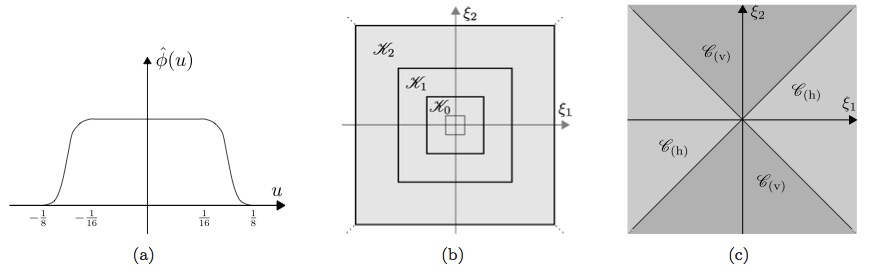
\includegraphics[width=0.9\textwidth]{./Diagrams/alphapartcones.jpg}
\caption{(a) Fourier transform of a Meyer scaling function. (b) Decomposition of the frequency plane by corona functions $W_j$ and $\Phi$. (c) Symmetric frequency decompositionby cones. Figure taken from \cite{Gitta-alpha} pp. 11}
\label{fig:separable_nonseparable}
\end{figure}

Lets introduce adapted versions of the usual shearing and scaling matrices,
$$
A_{\alpha,(h)}:=\left(\begin{matrix} 2 & 0 \\ 0 & 2^{\alpha/2}\end{matrix}\right) \quad \textrm{,}\quad S_{(h)}:=\left(\begin{matrix} 1 & 1\\ 0 & 1\end{matrix}\right)
$$
$$
A_{\alpha,(v)}:=\left(\begin{matrix}2^{\alpha/2} & 0 \\ 0 & 2 \end{matrix}\right)\quad \textrm{,}\quad S_{(v)}:=\left(\begin{matrix} 1 & 0 \\ 1 & 1\end{matrix}\right)
$$

where $\alpha\in (-\infty,2)$ is the \textit{scaling parameter}, $A_{j,\alpha,(\iota)}:=A^j_{\alpha,(\iota)}$ and $S_{k,(\iota)}:=S^k_{(\iota)}$ for $\iota\in\{h,v\}$. The adapted \textit{cone functions} are given by
$$
V_{(h)}(\xi):=v(\xi_2/\xi_1)\textrm{,}\quad V_{(v)}(\xi):=v(\xi_1/\xi_2)\textrm{,}\quad \xi\in\mathbb{R}^2.
$$
Lets define now the ingredients of a universal shearlet system.

\bigskip

\begin{defn}
\label{def:alpha31}
Let $\Phi$, $W$, $V_{(h)}$, $V_{(v)}\in L^2(\mathbb{R}^2)$ be defined as before.
\begin{enumerate}
\item[1.] \textbf{Coarse scaling functions}: For $k\in\mathbb{Z}^2$, we set 
$$
\psi_{-1,k}:=\Phi(x-k)\textrm{,}\quad x\in\mathbb{R}^2.
$$
\item[2.] \textbf{Interior shearlets}: Let $\alpha\in (-\infty,2)$, $j\in\mathbb{N}_0$, $k\in\mathbb{Z}$ with $|k|< 2^{(2-\alpha)j/2}$, $m\in\mathbb{Z}^2$ and $\iota\in\{h,v\}$. The shearlets will be given by 

\begin{equation}
\label{eq:alpha35}
\hat{\psi}^{\alpha,(\iota)}_{j,k,m}(\xi):=2^{-(\alpha+2)j/4}W(2^{-j}\xi)V_{(\iota)}(\xi^{\top} A_{-j,\alpha,(\iota)}S_{-k,(\iota)})e^{-2\pi i\xi^{\top}A_{-j,(\iota)}S_{-k,(\iota)}}\textrm{,}\quad \xi\in\mathbb{R}^2
\end{equation}

\item[3.] \textbf{Boundary shearlets}: For $\alpha\in(-\infty,2)$, $j\geq 1$, $k=\pm\lceil 2^{(2-\alpha)j/2}\rceil$ and $k\in\mathbb{Z}^2$, we define
\begin{equation}
\label{eq:alpha36}
\hat{\psi}_{j,k,m}^{\alpha}:=
\begin{cases}
2^{-(\alpha+2)j/4-1/4}W(2^{-j}\xi)V_{(h)}(\xi^{\top} A_{-j,\alpha,(h)}S_{-k,(\iota)})e^{-\pi i\xi^{\top}A_{-j,\alpha,(h)}S_{-k,(h)}m}\textrm{,}\quad \xi\in\mathcal{C}_{(h)},\\
2^{-(\alpha+2)j/4-1/4}W(2^{j}\xi)V_{(v)}(\xi^{\top}A_{-j,\alpha,(v)}S_{-k,(v)})e^{-\pi i\xi^{\top}A_{-j,\alpha,(v)}S_{-k,(h)}m}\textrm{,}\quad \xi\in\mathcal{C}_{(v)}
\end{cases}
\end{equation}
and in the case $j=0$, $k=\pm 1$, we define
$$
\hat{\psi}^{\alpha}_{0,k,m}:=
\begin{cases}
W(\xi) V_{(h)}(\xi^{\top}S_{-k,(h)})e^{-2\pi i\xi^{\top}m}\textrm{,}\quad \xi\in\mathcal{C}_{(h)}\textrm{,}\\
W(\xi)V_{(v)}(\xi^{\top}S_{-k,(v)})e^{-2\pi i\xi^{\top}m}\textrm{,}\quad \xi\in\mathcal{C}_{(v)}.
\end{cases}
$$
One can compare this definition of shearlet system with the Definition~\ref{def:cone_shearlets} of classical cone-adapted shearlet system and see that in the case of $\alpha = 1$ both are the same. The Fourier transform $\hat{\psi}_{j,k,m}^{\alpha,(h)}$ has compact support in the trapezoidal region

\begin{equation}
\label{eq:alpha37}
\{\xi\in\mathbb{R}^2|\xi_1\in[-2^{j-1},2^{j-1}]\setminus (-2^{j-2},2^{j-2}),||\xi_2/\xi_1-k2^{-(2-\alpha)j/2}|\leq 2^{-(2-\alpha)j/2}\}.
\end{equation}
\end{enumerate}
\end{defn}

\bigskip

Since the boundary shearlets were defined piecewise, smoothness (of the Fourier transforms) is not guaranteed for all $\alpha\in (-\infty,2)$. The exponent $2^{(2-\alpha)j/2}$ needs to be necessarily integer-valued when analyzing the first partial derivatives of eq.~\ref{eq:alpha36}. To satisfy this for every $j\in\mathbb{Z}$, we would have to restrict the set of admissible $\alpha$ to the set of integers; but this would not give us the arbitrary scaling behavior that we are looking for. To overcome this issue one can relax the condition of a globally fixed $\alpha$ and, introduce a \textit{separate} scaling parameter $\alpha_j$ on each scale. The universal shearlet system will be associated with a whole sequence $(\alpha_j)_{j\in\mathbb{N}_0}\subset\mathbb{R}$. In this setting the set of admissible scaling parameters can be substantially enlarged since we have $(2-\alpha_j)j/2\in\mathbb{Z}$ whenever $\alpha_j$ is multiple of $2/j$. 

\bigskip

\begin{defn}
\label{def:alpha32}
A sequence $(\alpha_j)_{j\in\mathbb{N}_0}\subset\mathbb{R}$ is called a scaling sequence if 
$$
\alpha_j\in A_j:=\left \{\frac{2n}{j}\big| n\in\mathbb{Z},n\leq j-1\right \}=\left \{\ldots,-\frac{4}{j},-\frac{2}{j},0,\frac{2}{j},\ldots,1-\frac{2}{j}\right \}
$$
\end{defn}

\bigskip

\begin{defn}
\label{def:alpha33}
Let $(\alpha_j)_{j\in\mathbb{N}_0}$ be a \textit{scaling sequence}. Then we define the associated universal-scaling shearlet system, or shorter, universal shearlet system, by
$$
\mathcal{SH}(\phi,v,(\alpha_j)_j):=\mathcal{SH}_{\text{Low}}(\phi)\cup\mathcal{SH}_{\text{Int}}(\phi,v,(\alpha_j)_j)\cup\mathcal{SH}_{\text{Bound}}(\phi,v,(\alpha_j)_j),
$$
where
$$
\begin{aligned}
\mathcal{SH}_{\text{Low}}(\phi)&:=\{\psi_{-1,m}|m\in\mathbb{Z}^2\}\\
\mathcal{SH}_{\text{Int}}(\phi,v,(\alpha_j)_j)&:=\{\psi_{j,k,m}^{\alpha_j,(\iota)}|j\geq 0,|m|< 2^{(2-\alpha_j)j/2},m\in\mathbb{Z}^2,\iota\in\{h,v\}\},\\
\mathcal{SH}_{\text{Bound}}(\phi,v,(\alpha_j)_j)&:=\{\psi_{j,k,m}^{\alpha_j}|j\geq 0,|k|=\pm 2^{(2-\alpha_j)j/2},m\in\mathbb{Z}^2\}.
\end{aligned}
$$

\end{defn}

\bigskip

Since the elements of a scaling sequence $\alpha_j$ can be chosen independently for each scaling level and, in particular, the sequence $(\alpha_j)_j$ does not need to converge; this premits a faithful implementation of the universal shearlet transform; this is already implemented in the toolbox used in this thesis (Shearlab.jl) one determines the total number of shearings (on each scale) first given by $|k|\leq \lceil 2^{(2-\alpha_j)j/2}\rceil$, rather that selecting a fixed $\alpha_j$. We are ready to prove the main property of the universal shearlet system, i.e.\ its character of frame.

\begin{thm}[Universal shearlet frames]
\label{thm:alpha34}
Let $(\alpha_j)_{j}$ be a scaling sequence and $\mathcal{SH}(\phi,v,(\alpha_j)_j)$ be an associated universal shearlet system. Then $\mathcal{SH}(\phi,v,(\alpha_j)_j)$ constitutes a Parseval frame for $L^2(\mathbb{R}^2)$ consisting of band-limited Schwartz functions. Moreover, the interior and boundary shearlets have infinitely  many vanishing moments. 
\end{thm}
\begin{proof}
Lets proceed with the proof of the different properties required.
\begin{itemize}
\item\textit{Band-limiting and vanishing moment property:} Observing that $(0,0)\notin \text{supp}W_k\subset \mathcal{K}_j$ which immediately follows from Definition~\ref{def:alpha31}.
\item\textit{Smoothness:} Due to the band-limiting of $\mathcal{SH}(\phi,v,(\alpha_j)_j)$, it is sufficient to show that the Fourier transforms of the elements are smooth. This will imply that $\mathcal{SH}(\phi,v,(\alpha_j)_j)\subset \mathcal{S}(\mathbb{R}^2)$. 

\bigskip

The smoothness of $\mathcal{SH}_{\text{Low}}(\phi,v,(\alpha_j)_j)$ and $\mathcal{SH}_{\text{Int}}(\phi,v,(\alpha_j)_j)$ are induced by their smooth defining functions $\phi$ and $v$. We still need to consider elements $\psi^{\alpha_j}_{j,k,m}\in\mathcal{SH}_{\text{Bound}}(\phi,v,(\alpha_j)_j)$. In the interior of $\mathcal{C}_{(h)}$ and $\mathcal{C}_{(v)}$, the smoothness is again obvious. Thus, we only need to analyze the boundary lines of the cones which are given by $\{|\xi_1|=|\xi_2|\}$.

\bigskip

Lets use the shortcut $k_j:=2^{(2-\alpha_j)j/2}$ for the maximal shearing number (on scale $j$) and simplify the definition of $\hat{\psi}_{j,k,m}^{\alpha_j}$ (for $j\geq 1$):

\begin{equation}
\label{eq:alpha71}
\hat{\psi}^{\alpha_j}_{j,k,m}(\xi)=2^{-\frac{(2+\alpha_j)j}{4}-\frac{1}{4}}\cdot
\begin{cases}
W(2^{-j}\xi)v(k_j(\xi_2/\xi_1-1))&e^{-\pi i[2^{-j}\xi_1 m_1+2^{-\alpha_j j/2}(\xi_2-\xi_1)m_2]}\\
& \textrm{,}\quad \xi\in\mathcal{C}_{(h)},\\
W(2^{-j}\xi)v(k_j(\xi_1/\xi_2-1))&e^{-\pi i[2^{-j}\xi_1 m_1+2^{-\alpha_j j/2}(\xi_1-\xi_1)m_2]}\\
&\textrm{,}\quad \xi\in\mathcal{C}_{(v)},
\end{cases}
\end{equation}

In the case of $\xi_1=\pm \xi_2$, both terms coincide implying the continuity of $\hat{\psi}_{j,k,m}^{\alpha_j}$. By the same argument, the continuity of $\hat{\psi}_{j,-k_j,m}^{\alpha_j}$ is cerified. Next we comput the partial derivatives of both terms in eq.~\ref{eq:alpha71} which are given by

\begin{equation}
\label{eq:alpha72}
\begin{aligned}
\frac{\partial}{\partial\xi_1}\big|_{\xi_1=\xi_2}[W(2^{-j}\xi)v(k_j(\xi_2/\xi_1-1))&e^{-\pi i[2^{-j}\xi_1m_1+2^{-\alpha_j j/2}(\xi_2-\xi_1)m_2]}]\\
=2^{-j}\frac{\partial W}{\partial\xi_1}(2^{-j}\xi_1,2^{-j}\xi_1)v(0)&e^{-2^{-j}\pi i\xi_1 m_1}-\frac{k_j}{\xi_1}W(2^{-j}\xi_1,2^{-j}\xi_1)v'(0)e^{-2^{-j}\pi i\xi_1 m_1}\\
&-\pi i(2^{-j}m_1-2^{-\alpha_j j/2}m_2)W(2^{-j}\xi_1,2^{-j}\xi_1)v(0)\\
&\quad \cdot e^{-2^{-j}\pi i\xi_1 m_1}
\end{aligned}
\end{equation}

and

\begin{equation}
\label{eq:alpha73}
\begin{aligned}
&\frac{\partial}{\partial\xi_1}\big|_{\xi_1=\xi_2}[W(2^{-j}\xi)v(k_j(\xi_1/\xi_2-1))e^{-\pi i[2^{-j}\xi_1m_1+2^{\alpha_j j/2}(\xi_2-\xi_1)m_2]}]\\
&=2^{-j}\frac{\partial W}{\partial\xi_1}(2^{-j}\xi_1,2^{-j}\xi_1)v(0)e^{-2^{-j}\pi i\xi_1 m_1}+\frac{k_j}{\xi_1}W(2^{-j}\xi_1,2^{-j}\xi_1)v'(0)e^{-2^{-j}\pi i\xi_1 m_1}\\
&\quad-\pi i(2^{-j}m_1-2^{-\alpha_j j/2}m_2)W(2^{-j}\xi_1,2^{-j}\xi_1)v(0)e^{-2^{-j}\pi i\xi_1 m_1}
\end{aligned}
\end{equation}
These two expressions coincide, since by definition $v'(0)=0$. The same can be done in a similar way for the partial derivative with respect to $\xi_2$, and by obvious modifications, one verifies the smoothness for $\hat{\psi}_{j,-k_j,m}^{\alpha_j}$ as well as for the case $j=0$. Finally, the differentiability of higher order is proven by induction and successive use of eq.~\ref{eq:alpha34}.

\item\textit{Parseval frame property:} Let $f\in L^2(\mathbb{R}^2)$ be arbitrary. Lets condiser the different parts of $\mathcal{SH}(\phi,v,(\alpha_j)_j)$ separately:

\begin{enumerate}
\item[\textbf{Case 1}] Boundary shearlets with $j\geq 1$: By Plancherel's Theorem, we get
\begin{equation}
\label{eq:alpha74}
\begin{aligned}
\sum_{m\in\mathbb{Z}^2} |\langle f,\psi_{j,k,m}^{\alpha_j}&\rangle|^2=\sum_{k\in\mathbb{Z}^2}\langle \hat{f},\hat{\psi}_{j,k,m}^{\alpha_j}\rangle |^2 =\sum_{k\in\mathbb{Z}^2}\bigg|\int_{\mathbb{R}^2}2^{-(2+\alpha_j)j/4-1/2}\hat{f}(\xi)W(2^{-j}\xi)\\
ep^{\pi i\xi^{\top}A_{-j,\alpha_j,(h)}S_{-k_j,(h)}m}&\times[\chi_{\mathcal{C}_{(h)}}V_{(h)}(\xi^{\top}A_{-j,\alpha_j,(h)}S_{-k_j,(h)})+\chi_{\mathcal{C}_{(v)}}(\xi)V_{(v)}(\xi^{\top}A_{-j,\alpha_j,(v)}S_{k_j,(v)})]d\xi\bigg|^2
\end{aligned}
\end{equation}
In order to apply the Parseval's identity, we can make use of that
$$
\eta^{\top}:=2^{-1}\xi^{\top}A_{-j,\alpha_{j},(h)}S_{-k_j,(h)}\Leftrightarrow \xi=\xi(\eta)=(2^{j+1}\eta_1,2^{j+1}\eta_1+2^{\alpha_j j/2+1}\eta_2).
$$
Then the equation~\ref{eq:alpha74} will have the form
$$
\begin{aligned}
V_{(h)}\left(\xi^{\top}A_{j,\alpha_j,(h)}S_{-k_j,(h)}\right)&=v\left(\begin{matrix}\eta_2\\ \eta_1\end{matrix}\right),\\
V_{(v)}\left(\xi^{\top}A_{-j,\alpha_j,(v)}S_{-k_j,\alpha_j,(v)}\right)&=v\left(2^{(2-\alpha)j/2}(\xi_1/\xi_2-1)\right) = v\left(-\frac{\eta_2}{\eta_1+2^{(\alpha_j-2)j/2}\eta_2}\right),\\
W(2^{-j}\xi)=W\left(2\eta_1,2[\eta_1+2^{(\alpha_j-2)j/2}\eta_2]\right).
\end{aligned}
$$
By equation~\ref{eq:alpha31}, the mapping $(\eta_1,\eta_2)\mapsto W(2\eta_1,2[\eta_1+2^{(\alpha_j-2)j/2}\eta_2])$ is supported in the strip $\{|\eta_1|\leq 1/4\}$. Since $\text{supp}v\subset [-1,1]$, we have that the mappings
$$
\begin{aligned}
(\eta_1,\eta_2)\mapsto U_{(h),j}(\eta)&:=W(2\eta_1,2[\eta_1+2^{(\alpha_j-2)j/2}\eta_2])v\left(\frac{\eta_2}{\eta_1}\right)\\
(\eta_1,\eta_2)\mapsto U_{(v),j}(\eta)&:=W(2\eta_1,2[\eta_1+2^{(\alpha_j-2)j/2}\eta_2])v\left(-\frac{\eta_2}{\eta_1+2^{(\alpha_j-2)j/2}\eta_2}\right)
\end{aligned}
$$
are supported in the square $Q^2:=[-1/2,1/2]^2$. Here, we used
$$
\begin{aligned}
\big|-\frac{\eta_2}{\eta_1+2^{(\alpha_j-2)j/2}\eta_2}\bigg|\leq 1&\Longrightarrow \bigg|\frac{\eta_2}{\eta_1}\bigg|\leq \bigg| 1+2^{(\alpha_j-2)j/2}\frac{\eta_2}{\eta_1}\bigg|\leq 1+2^{(\alpha_j-2)j/2}\bigg|\frac{\eta_2}{\eta_1}\bigg|\\
&\Longrightarrow \bigg|\frac{\eta_2}{\eta_1}\bigg| \leq\frac{1}{1-2^{(\alpha_j-2)j/2}}\leq 2
\end{aligned}
$$
where in the last inequality we used $\alpha_j\leq 1-2/j$. With this observation, we can continue in~\ref{eq:alpha74} by
$$
\begin{aligned}
&\sum_{k\in\mathbb{Z}^2}|\langle f,\psi_{j,k_j,m}^{\alpha_j}\rangle|^2\\
&=\sum_{k\in\mathbb{Z}^2}\bigg|\int_{Q^2}2^{(2+\alpha_j)j/4+1/4}\hat{f}(\xi(\eta))\left[ \chi_{\mathcal{C}_{(h)}}(\xi(\eta))U{(h),j}(\eta)+\chi_{\mathcal{C}_{(v)}}(\xi(\eta))U_{(v),j}(\eta)\right]e^{2\pi i\eta^{\top}m}d\eta\bigg|^2\\
&=\int_{Q^2}2^{(2+\alpha_j)j/2+1/2}|\hat{f}(\xi(\eta))|^2\bigg|\xi_{\mathcal{C}_{(h)}}(\xi(\eta))U_{(h),j}(\eta)+\xi_{\mathcal{C}_{(v)}}(\xi(\eta))U_{(v),j}(\eta)\bigg|^2d\eta\\
&=\int_{\mathcal{C}_{(h)}}|\hat{f}(\xi)|^2|W(2^{-j}\xi)|^2|v(k_j(\xi_2/\xi_1-1))|^2+\int_{\mathcal{C}_{(v)}}|\hat{f}(\xi)|^2|W(2^{-j}\xi)|^2|v(k_j(\xi_1/\xi_2-1))|^2d\xi.
\end{aligned}
$$
Similarly we can get
$$
\begin{aligned}
\sum_{k\in\mathbb{Z}^2}|\langle f,\psi_{j,k_j,m}^{\alpha_j}\rangle|^2&=\int_{\mathcal{C}_{(h)}}|\hat{f}(\xi)|^2|W(2^{-j}\xi)|^2|v(k_j(\xi_2/\xi_1+1))|^2d\xi\\
&+\int_{\mathcal{C}_{(v)}}|\hat{f}(\xi)|^2|W(2^{-j}\xi)|^2|v(k_j(\xi_1/\xi_1+1))|^2d\xi
\end{aligned}
$$
which finishes the first case.

\item[\textbf{Case 2}] Boundary shearlets with $j=0$: Since $\text{supp}W\subset Q^2$, we obtain
$$
\begin{aligned}
&\sum_{k\in\mathbb{Z}^2}|\langle f,\psi_{0,\pm 1,m}^{\alpha_j}\rangle|^2=\sum_{k\in\mathbb{Z}^2}|\langle \hat{f},\hat{\psi}_{0,\pm 1,k}^{\alpha_j}\rangle|^2\\
&=\sum_{k\in\mathbb{Z}^2}\bigg|\int_{Q^2}\hat{f}(\xi)W(\xi)\left[\chi_{\mathcal{C}_{(h)}}v\left(\frac{\xi_2}{\xi_1}\mp 1\right) +\chi_{\mathcal{C}_{(v)}}(\xi)\left(\frac{\xi_1}{\xi_2}\mp 1\right)\right]e^{2\pi i\xi^{\top}m}d\xi\bigg|^2\\
&=\int_{\mathcal{C}_{(h)}}|\hat{f}(\xi)|^2|W(\xi)|^2\bigg| v\left(\frac{\xi_2}{\xi_1}\mp 1\right)\bigg|^2d\xi+\int_{\mathcal{C}_{(v)}}|\hat{f}(\xi)|^2|W(\xi)|^2\bigg|v\left(\frac{\xi_1}{\xi_2}\mp 1\right)\bigg|^2d\xi
\end{aligned}
$$

\item[\textbf{Case 3}] Interior shearlets: The substitution $\eta^{\top}=\xi^{\top}A_{-j,\alpha_j,(\iota)}S_{-k,(\iota)}$, for $|k|<k_j$, $\iota\in\{h,v\}$ yields
$$
\begin{aligned}
\sum_{k\in\mathbb{Z}^2}|\langle f,\psi_{j,k,m}^{\alpha_j,(h)}\rangle |^2 &= \int_{\mathbb{R}^2}|\hat{f}(\xi)|^2|W(2^{-j}\xi)|^2 \bigg|v\left(k_j\frac{\xi_2}{\xi_1}-k\right)\bigg|^2d\xi,\\
\sum_{k\in\mathbb{Z}^2}|\langle f,\psi_{j,k,m}^{\alpha_j,(v)}\rangle |^2 &= \int_{\mathbb{R}^2}|\hat{f}(\xi)|^2|W(2^{-j}\xi)|^2\bigg|v\left(k_j\frac{\xi_1}{\xi_2}-k\right)\bigg|^2d\xi,
\end{aligned}
$$

\item[\textbf{Case 4}] Coarse scaling functions: Since $\text{supp}\Phi\subset Q^2$, we have
$$
\sum_{k\in\mathbb{Z}^2}|\langle f,\psi_{-1,m}\rangle|^2=\sum_{k\in\mathbb{Z}^2}\bigg| \int_{Q^2}\hat{f}(\xi)\hat{\Phi}(\xi) e^{-2\pi i\xi^{\top}m}d\xi\bigg|^2 = \int_{\mathbb{R}^2}|\hat{f}(\xi)|^2|\hat{\Phi}(\xi)|^2d\xi
$$
\end{enumerate}
Finally, using \textbf{Case 1} to \textbf{Case 2} we can conclude that 

$$
\begin{aligned}
&\sum_{\psi\in\mathcal{SH}(\phi,v,(\alpha_j)_j)}|\langle f,\psi\rangle |^2\\
&=\sum_{k\in\mathbb{Z}^2}\left( |\langle f,\psi_{-1,m}\rangle|^2+\sum_{\iota\in\{h,v\}}\sum_{j\in\mathbb{N}_0}\sum_{|k|<k_j}|\langle f,\psi_{j,k,m}^{\alpha_j,(\iota)}\rangle|^2+\sum_{j\in\mathbb{N}_0}\sum_{k=\pm k_j}|\langle f,\psi_{j,k,m}^{\alpha_j}\rangle |^2 \right)\\
&=\int_{\mathbb{R}^2}|\hat{f}(\xi)|^2|\hat{\Phi}(\xi)|^2d\xi\\
&+\int_{\mathbb{R}^2}|\hat{f}(\xi)|^2\sum{j\in\mathbb{N}_0}|W(2^{-j}\xi)|^2\left[ \sum_{|k|<k_j}\bigg| v\left( k_j\frac{\xi_2}{\xi_1}-k\right)\bigg|^2+\sum_{|k|<k_j}\bigg| v\left(k_j\frac{\xi_1}{\xi_2}-k\right)\bigg|^2\right] d\xi\\
&+\int_{\mathbb{C}_{(h)}}|\hat{f}(\xi)|^2\sum_{j\in\mathbb{N}_0}|W(2^{-j}\xi)|^2|v(k_j(\xi_2/\xi_1-1))|^2d\xi\\
&+\int_{\mathbb{C}_{(v)}}|\hat{f}(\xi)|^2\sum_{j\in\mathbb{N}_0}|W(2^{-j}\xi)|^2|v(k_j(\xi_1/\xi_1-1))|^2d\xi\\
&+\int_{\mathbb{C}_{(h)}}|\hat{f}(\xi)|^2\sum_{j\in\mathbb{N}_0}|W(2^{-j}\xi)|^2|v(k_j(\xi_2/\xi_1+1))|^2d\xi\\
&+\int_{\mathbb{C}_{(v)}}|\hat{f}(\xi)|^2\sum_{j\in\mathbb{N}_0}|W(2^{-j}\xi)|^2|v(k_j(\xi_1/\xi_1+1))|^2d\xi\\
&=\int_{\mathbb{R}^2}|\hat{f}(\xi)|^2|\hat{\Phi}(\xi)|^2d\xi+\int_{\mathbb{R}^2}|\hat{f}(\xi)|^2\sum_{j\in\mathbb{N}_0}|W(2^{-j}\xi)|^2\times \\
&\quad \times \left[ \chi_{\mathcal{C}_{(h)}}(\xi)\sum_{|k|\leq k_j}\bigg| v\left( k_j\frac{\xi_2}{\xi_1}-k\right)\bigg|^2+\chi_{\mathcal{C}_{(v)}}(\xi)\sum_{|k|\leq k_j}\bigg| v\left( k_j\frac{\xi_1}{\xi_2}-k\right)\bigg|^2\right]d\xi\\
&\underset{~\ref{eq:alpha31}}{=}\int_{\mathbb{R}^2}|\hat{f}(\xi)|^2\left[|\hat{\Phi}(\xi)|^2+\sum_{j\in\mathbb{N}_0}|W(2^{-j}\xi)|^2\right]d\xi = ||\hat{f}||^2_{L^2(\mathbb{R}^2)}=||f||^2_{L^2(\mathbb{R}^2)}
\end{aligned}
$$
Then we have the proof finished. 
\end{itemize}
\end{proof}

\bigskip

Now that we know that the general shearlet system forms a frame, we can introduce a simpler idea with $\alpha$ fixed, the so called $\alpha$-Shearlets.

\begin{defn}[$\alpha$-Shearlets]
\label{def:alphashearlets}
For $\phi,\psi,\tilde{\psi}\in L^2(\mathbb{R}^2)$, $\alpha\in (-\infty,2)$ and $c=(c_1,c_2)\in (\mathbb{R}^+)^2$, the \textit{$\alpha$-shearlets system} $\mathcal{SH}(\phi,\psi,\tilde{\psi};\alpha,c)$ is defined as
$$
\mathcal{SH}(\phi,\psi,\tilde{\psi};\alpha)=\Phi(\phi;c_1)\cup\Psi(\psi;\alpha,c)\cup\tilde{\Psi}(\tilde{\psi};\alpha,c),
$$
where
$$
\begin{aligned}
\Phi(\phi;c_1)&=\{\phi_m=\phi(\cdot-c_1m):m\in\mathbb{Z}^2\}\\
\Psi(\psi;\alpha,c):=\{\psi_{j,k,m}&=2^{(\alpha+1)j/4}\psi(S_{k,(h)}A_{j,\alpha,(h)}\cdot-M_{c,(h)}m)\textrm{:}j\geq 0,|k|\leq \lceil 2^{(\alpha-1)j/2}\rceil,m\in\mathbb{Z}^2\},\\
\tilde{\Psi}(\tilde{\psi};\alpha,c):=\{\tilde{\psi}_{j,k,m}&=2^{(\alpha+1)j/4}\tilde{\psi}(S_{k,(v)}A_{j,\alpha,(v)}\cdot-M_{c,(v)}m)\textrm{:}j\geq 0,|k|\leq \lceil 2^{(\alpha-1)j/2}\rceil,m\in\mathbb{Z}^2\},\\
\end{aligned}
$$
where $M_{c,(h)}=\text{diag}(c_1,c_2)$ and $M_{c,(v)}=\text{diag}(c_2,c_1)$.
\end{defn}

Let $\alpha\in (-\infty,2)$, and recall the form of the scaling sequences set $A_j$ from definition~\ref{def:alpha32}, we choose $(\alpha_j)_j$ then to be the best possible approximation of $\alpha$, 
$$
\alpha_j:=\underset{\tilde{\alpha}_j\in A_j}{\text{argmin}}|\tilde{\alpha}_j-\alpha|\textrm{,}\quad j\geq 1.
$$

It is easy to verify that $2^{\alpha_j j/2}\in\Theta(2^{\alpha_j/2})$ as $j\longrightarrow \infty$. Then the corresponding universal shearlet system (or universal-scaling shearlet system) $\mathcal{SH}(\phi,v,(\alpha_j)_j)$ has asymptotically the same scaling behavior as $\alpha$-shearlets; for further analysis of $\alpha$-shearlets and universal shearlet system we recommend to check \cite{Gitta-alpha} and \cite{firstalpha}. This generalized theory is very useful in the case that we want to have more freedom on the level of anisotropy of the features of some signal we want to analyze; this also will give us a general framework of sparse representation of different type of features in natural images and videos, the sparse character of the representations let us use the shearlet transform for typical image processing tasks as denoising and inpainting; the latter plays an important role in the light field recovery method presented in this thesis and therefore we will explore it in more detail on the next section.

\section{Image inpainting using $\alpha$-Shearlets}

On the last chapter we explained how one can optimize the light field acquisition by using sparse acquisition setups that reduces the number of images of the scene (sampling rate) that one needs to acquire and still be able to recover the light field, this also reduces the complexity of the EPIs acquisition algorithm but adds a new problem; the EPIs obtained by this sparse acquisition technique are as well sparse so one will truncated straight lines instead of straight lines (see Figure~\ref{fig:sparse_EPI}). 

\begin{figure}[h!]
\centering
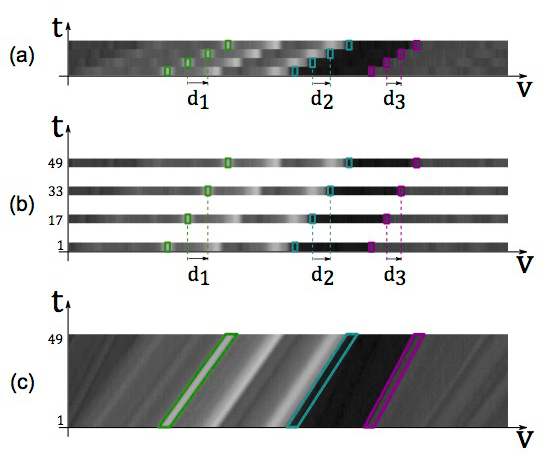
\includegraphics[width=0.6\textwidth]{./Diagrams/sparse_EPI.jpg}
\caption{(a) EPI for a coarsely sampled light field; (b) Correspondeing partially defined densely sampled EPI; (c) Ground truth densely sampled EPI, can be obtaied by inpainting. Figure taken from \cite{LF-Shearlets} pp. 6}
\label{fig:sparse_EPI}
\end{figure}

One would like to recover the lost sections of the EPIs, this task is present in different applications on data processing, since frequently the technologies of data acquisition fails resulting on missing traces; in imaging sicence, this task is referred as \textit{inpainting} by the similiraty of the physical task of restoring a painting. 

\bigskip

There are different algorithmical approaches to the inpainting task; the algorithms based on variational approaches which propagate information from the boundaries and try to guarantee smoothness (see \cite{Ballester}). Another approach is based on applied harmonic analysis combined with ideas of compressed sensing, assuming that certain representation systems provide sparse approximations of the original image, most of the approaches assume that one knows the position and shape of the lost areas (referred as masks).

\bigskip

In this thesis we will follow the second approach exploiding the sparse representation characteristics of the shearlet systems to inpaint epipolar plane images obtained from a sparsely sampled light field; using a combination of harmonic analysis and also a $\ell^1$ minimization technique widely used in compressed sensing. 

\bigskip

Before explaining the particular case of inpainting algorithm that we will work with it is worthwhile to present a general abstract framework of inpainting to grow some intuition. For this we need a separable Hilbert space $\mathcal{H}$. Let $x^0\in\mathcal{H}$ the undamaged (original) \textit{signal} that we want to recover. We will also assume that $\mathcal{H}$ decomposes into an orthogonal sum of two closed subspaces, that we will call the \textit{known part} and the \textit{missing part}, 

$$
\mathcal{H}=\mathcal{H}_K\oplus\mathcal{H}_M=P_K\mathcal{H}\oplus P_M\mathcal{H}
$$

where $P_K$ and $P_M$ are the orthogonal projection operator to the respective space. The inpainting of $x^0$ will be then translated to: "Given a corrupt signal $P_Kx^0$, recover the missing part $P_Mx^0$. 

\bigskip

In the case of image inpainting, we will consider a continuous image model, where $\mathcal{H}=L^2(\mathbb{R}^2)$, where the missing space is $H_M=L^2(\mathcal{M})$ for some measurable set $\mathcal{M}\subset\mathbb{R}^2$, seen as a mask covering the corrupted parts of the painting. In the next we will make further assumptions on the signal and missing space.

\bigskip

We will assume that the signal $x^0$ can be efficiently represented by some Parseval frame $\Phi=(\phi_i)_{i\in I}$ for $\mathcal{H}$, at practical applications this assumption is reasonable since we already mentioned that natural images represented by cartoon-like functions are optimally represented by directional systems as shearlets or curvelets. In the classical theory of sparse representations, this is translated as asking for the solution of the $\ell^0$-minimization problem

\begin{equation}
\label{eq:alpha21}
\underset{c\in\ell^2(I)}{\min}||c||_{\ell^0(I)}\quad\textrm{subject to}\quad x^0=T_{\Phi}^*c=\sum_{i\in I}c_i\phi_i
\end{equation}

where the operator $T^*_{\Phi}$ is the so-called synthesis operator associated to the frame, then equation~\ref{eq:alpha21} tries to find a synthesis sequence of $x^0$ that has as few as possible non-zero elements measured by $||c||_0:=\#\{c_i|c_i\neq 0\}$. This minimization problem is not convex which represents a big complexity issue in the solution method; we will then follow a new strategy called \textit{analysis approach}.

\bigskip

In the \textit{analysis approach} we will consider \textit{analysis coefficients} given by the \textit{analysis operator} $T_{\Phi}x^0=(\langle x^0,\phi_i\rangle)_{i\in I}$, since the frame is assumed to obey the Parseval property, we can perform the reconstruction by $x^0=T^*_{\Phi}(\langle x^0,\phi_i\rangle)_{i\in I}=\sum_{i\in I}\langle x^0,\phi\rangle\phi_i$. $\Phi$ is not necessarily a basis, $T_{\Phi}x^0$ might not be a solution of~\ref{eq:alpha21}, so is not yet clear what it means to give a sparse representation in the sense of the analysis approach; to make sanse of this we need to use some ideas of \textit{compressed sensing}.

\bigskip

To be able to use the \textit{analysis approach} we will introduce the next $\ell^1$-minimization algorithm:

\bigskip

\begin{algorithm}
    \SetKwInOut{Input}{Input}
    \SetKwInOut{Output}{Output}
		\SetKwInOut{Compute}{Compute}

    \Input{Corrupted signal $P_Kx^0\in\mathcal{H}_K$, Parseval frame $\Phi=(\phi_i)_{i\in I}$ for $\mathcal{H}$}
		\Compute{\begin{equation}
			x^*=\underset{x\in\mathcal{H}}{\text{argmin}}||T_{\Phi}x||_{\ell^1(I)} \quad\textrm{subject to}\quad P_Kx^0=P_Kx
			\tag{$\ell^1-\text{INP}$}
		\label{eq:alphal1}
		\end{equation}}
    \Output{recovered signal $x^*\in\mathcal{H}$}
    \caption{Inpainting via $\ell^1$-minimization}
		\label{alg:alpha21}
\end{algorithm}

\bigskip

In other words, Algorithm~\ref{alg:alpha21} minimizes the $\ell^1$-norm among all possible reconstruction candidates, which is the set of all signals coinciding with $x^0$ on $\mathcal{H}_K$. In the case where the undamaged signal $x^0$ is sufficiently sparsified by $\Phi$, and then an small $\ell^1$-norm of $T_{\Phi}x^0$, the solution $x^*$ will provide a good reconstruction of the important features on $x^0$.

\bigskip

We would like to prove some error estimates for the recovery by Algorithm~\ref{alg:alpha21}, for this, we will introduce some analysis tools that will also give us further insight about the structure of the proposed abstract model.

\bigskip

\begin{defn}[$\delta$-cluster sparsity]
\label{def:alpha22}
Let $\delta>0$ and $\Gamma\subset I$. A signal $x\in\mathcal{H}$ is called $\delta$-clustered sparse in $\Phi$ with respect to $\Gamma$, if
\begin{equation}
\label{eq:alpha22}
||\mathbf{1}_{\Gamma^c}T_{\Phi}x||_{\lambda^1}\leq \delta
\end{equation}
In this case, $\Gamma$ is sait to be $\delta$-cluster for $x$ in $\Phi$. 
\end{defn}

\bigskip

A signal will be $\delta$-clustered sparse if the analysis coefficients are highly concentrated on $\Gamma$. This definition will only have a useful meaning when $x$ is $\delta$-clustered sparse with respect to a small cluster $\Gamma$, and $\delta$ sufficiently small at the same time. Independently we can define the concept of \textit{cluster coherence}.

\bigskip

\begin{defn}[Cluster coherence]
Let $\Gamma\subset I$, the cluster coherence of $\Phi$ with respect to $\mathcal{H}_M$ and $\Gamma$ is given by 
$$
\mu_c(\Gamma,P_M\Phi):=\max_{j\in I}\sum_{i\in\Gamma}|\langle P_M\phi_i,P_M\phi_j\rangle|,
$$
where $P_M\Phi:=(P_M\phi_i)_{i\in I}$.
\end{defn}

\bigskip

The cluster coherence can be understood as an abstract measure for the gap size; we do not know $P_Mx^0$, so we would like to know the maximal amount of missing information. The Parseval expansion $x^0=\sum_{j\in I}\langle x^0,\phi_j\rangle \phi_j$ help us to estimate the analysis coefficientes of its projection onto $\mathcal{H}_M$:

\begin{equation}
\label{eq:alpha23}
|\langle P_Mx^0,\phi_i\rangle|\leq\sum_{i\in I}|\langle x^0,\phi_j\rangle||\langle P_M\phi_j,\phi_i\rangle|=\sum_{i\in I}|\langle x^0,\phi_j\rangle||\langle P_M\phi_j, P_M\phi_i\rangle|.
\end{equation}

The scalar products $|\langle P_M\phi_j,P_M\phi_i\rangle|$ broadly indicate how "correlated" the measurments with $\phi_i$ and $\phi_j$ are on $\mathcal{H}_M$. To compute the recovery error, it was proposed before (see \cite{Firstinpaint}) to estimate the ditance between $x^0$ and its $\ell^1$-recovery $x^*$ with the Hilbert norm. This worked well to estimate an upper bound, but to show an optimality result (lower bound), measuring $||\cdot||$ is not useful, since the Parseval property of $\Phi$ gives $||x^0-x^*||=||T_{\Phi}(x^0-x^*)||_{\ell^2}$, the $\ell^2$-norm in comparison with the $\ell^1$ has an averaging effect on the coefficientes, then some sparsity features might be hiddeng when using the Hilbert space norm. We will proposed a new norm to measure the error, the $\ell^1$-analysis norm.

\bigskip

\begin{defn}[$\ell^1$-analysis norm]
Let $x\in\mathcal{H}$ and $\Phi$ be a Parseval frame for $\mathcal{H}$. Then we define the $\ell^1$-analysis norm, with respect to $\Phi$, by
$$
||x||_{1,\Phi}:=||T_{\Phi}x||_{\ell^1}=||(\langle x,\phi_i\rangle)_{i\in I}||_{\ell^1}
$$
and the $\ell^1$-analysis space given by 
$$
\mathcal{H}_{1,\Phi}:=\{x\in \mathcal{H}|||x||_{1,\Phi}<\infty\}
$$
equipped with $||\cdot||_{1,\Phi}$
\end{defn}

Since $\Phi$ forms a Parseval frame, its analysis operator $T_{\Phi}$ is injective, and therefore the tuple $(\mathcal{H}_{1,\Phi},||\cdot||_{1,\Phi})$ defines a normed vector space, moreover
\begin{equation}
\label{eq:alpha24}
||x||=||T_{\Phi}x||_{\ell^2}\leq ||T_{\Phi}x||_{\ell^1}=||x||_{1,\Phi}
\end{equation}
then we have the embedding $\mathcal{H}_{1,\Phi}\hookrightarrow\mathcal{H}$, then, by picking $x=x^*-x^0$, we can conclude that small recovery errors in $\mathcal{H}_{1,\Phi}$ always imply small ones in $\mathcal{H}$. With this tools we can provide a estimate of the recovery error.

\begin{thm}
\label{thm:alpha25}
Let $\delta>0$ and $\Gamma\subset I$ be a $\delta$-cluster for $x^0$ in $\Phi$. Moreover, assume that $\mu_c(\Gamma,P_M\Phi)<1/2$. If $x^0\in\mathcal{H}_{1,\Phi}$ then the $\ell^1$-minimizer $x^*$ of the Algorithm~\ref{alg:alpha21} is also contained in $\mathcal{H}_{1,\Phi}$ and satisfies 
\begin{equation}
\label{eq:alpha25}
||x^*-x^0||_{1,\Phi}\leq \frac{2\delta}{1-2\mu_c(\Gamma,P_M\Phi)}
\end{equation}
\end{thm}
\begin{proof}
The proof can be found in \cite{Firstinpaint}.
\end{proof}

\bigskip

The Theorem~\ref{thm:alpha25} gives good estimates if $\Phi$ sparsifies $x^0$ and the size of the missing space, the latter measured in terms of cluster coherence is not too large. We would like to pick a cluster $\Gamma$ such that $x^0$ becomes $\delta$-clustered sparse for samll $\delta$ and at the same time $\mu_c$ shall not exceed the bound of $1/2$; even the concepts if cluster sparsity and cluster coherence were introduced independently, both notions are now joined together in terms of $\Gamma$; enlarging $\Gamma$ makes the Equation~\ref{eq:alpha25} true for smalle $\delta$, while $\mu_c(Gamma,P_MPhi)$ increases and could exceed $1/2$, this tell us that applying the Theorem~\ref{thm:alpha25} involves actually the fundamental task of choosing an appropriate cluster (see \cite{Firstinpaint} for a more detailed analysis). 

\bigskip

So far we have a general abstract framework for inpainting for Parseval frames, we would like to have an appropriate parseval frame to inpaint natural images (in the case of this thesis Epipolar Plane Images), in the sense that the recovery error is small; we have different options, for instance Universal Shearlet Systems and Wavelet Systems. Theorem~\ref{thm:alpha34} we know that for a scaling sequence $(\alpha_j)_j$ the related Universal Shearlet System $\mathcal{SH}(\phi,v,(\alpha_j)_j)$ form a Parseval frame for $L^2(\mathbb{R}^2)$ and that they behave asymptotically equally as the $\alpha$-Shearlets system $\mathcal{SH}(\phi,\psi,\tilde{\psi};\alpha)$, then the $\alpha$-Shearlets and the Universal Shearlet Transform can be used in the inpainting framework. In the case of the Wavelet Systems, they will also form a frame for $L^2(\mathbb{R}^2)$ under some assumptions on the mother wavelet function, the scaling and the translation parameter (see \cite{Mallat} pp. 202).

\bigskip

In order to compare the shearlets and the wavelets performance for inpaiting, we want to present a benchmark that is related to the principal problem of the thesis, that is the inpainting of sparse sampled epipolar plane images (see Figure~\ref{fig:sparse_EPI}). Cartoon-like images are we know are governed by edges, the image to be inpainted as a benchmark is a masked linear singularity that can be viewed as a strip; epipolar plane images corresponding to sparse sampled light fields have also strips as missing space so this example will be enough. Many details in the analysis will be ommited but they are well explained in \cite{Gitta-alpha}. 

\bigskip

As we cannot work on actual edges in $L^2(\mathbb{R}^2$ and other Lebesgue spaces since they have measure zero, we will work with a line-distribution given by $\omega\mathcal{L}$ acting on Schwartz functions $f\in\mathcal{S}(\mathbb{R}^2)$, i.e.\ $\omega\mathcal{L}\in \mathcal{S}'(\mathbb{R}^2)$, if $\text{supp }\omega\subset[-\rho,\rho]$ then its action will be defined by

$$
\langle \omega \mathcal{L},g\rangle = \int_{-\rho}^{\rho} \omega(x_1)g(x_1,0)dx_1 \textrm{,}\quad \forall g\in\mathcal{S}(\mathbb{R}^2)
$$

where $\omega$ is a smooth weight and $\rho>0$. The weight $\omega$ sets up the linear singularity that is smooth in the vertical direction, while the value of $\rho$ corresponds to the length of the singularity. We will mask the linear singularity (wheighted distribution) $\omega\mathcal{L}$ with the mask 

$$
M_h=\{(x_1,x_2)\in\mathbb{R}^2:|x_1|\leq h\}\textrm{,}\quad h>0
$$

The observed signal then is 
$$
f=\mathbf{1}_{\mathbb{R}^2\setminus M_h}\cdot \omega\mathcal{L}
$$ 

see Figure~\ref{fig:alpha6}. We decompose $\omega\mathcal{L}$ by the same subbands $F_j$, $\omega\mathcal{L}\mapsto \omega\mathcal{L}_j=\omega\mathcal{L}*F_j$, denote $h=h_j$ and set 

$$
f_j=\mathbf{1}_{\mathbb{R}^2\setminus M_{h_j}}\cdot \omega\mathcal{L}_j
$$

\begin{figure}[h!]
\centering
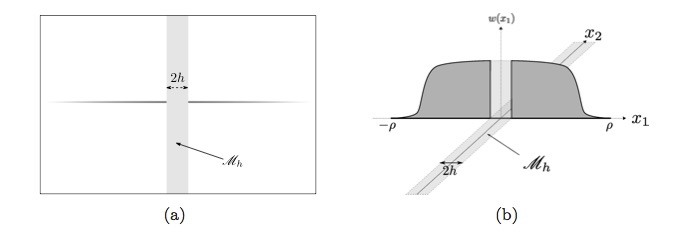
\includegraphics[width = 0.9 \textwidth]{./Diagrams/alpha6.jpg}
\caption{(a) Sketch of the corrupted modeling image, the line singularity has no "thickness" but some (gray-scale) intensity. (b) "Graph" of the corrupted line distribution $P_K\omega\mathcal{L}$ which is compactly supported on the $x_1$-axis. Figure taken from \cite{Gitta-alpha} pp. 15}
\label{fig:alpha6}
\end{figure}

\bigskip

Let $\{\psi_{\lambda}\}$ denote a particular wavelet Parseval frame and $\{ \sigma_{\eta}\}_{\eta}$ a particular shearlet Parseval frame (could be, classical shearlets, cone-adapted shearlets, $\alpha$-shearlets or universal shearlets). Then we can rewrite the minimization problem~\ref{eq:alphal1} as

$$
W_j=\underset{\tilde{W}_j}{\textrm{argmin}}||(\langle \tilde{W}_j,\psi_{\lambda}\rangle )_{\lambda}||_{\ell^1}\quad\textrm{subject to}\quad f_j=\mathbf{1}_{\mathbb{R}^2\setminus M_{h_j}}\cdot\tilde{W}_j
$$ 

for wavelet-based inpainting and 

$$
S_j=\underset{\tilde{S}_j}{\textrm{argmin}}||(\langle \tilde{S}_j,\sigma_{\eta}\rangle)_{\eta}||_{\ell^1}\quad \textrm{subject to}\quad f_j=\mathbf{1}_{\mathcal{R}^2\setminus M_{h_j}}\cdot\tilde{S}_j
$$

for the shearlet-based inpainting. Now we can state a Theorem that compares both systems in the inpainting task.

\begin{thm}
\label{thm:inpaintingwaveletsshearlets}
For $h_j=o(2^{-j})$ (the critical thresholding case) as $j\longrightarrow \infty$,
$$
\frac{||W_j-\omega\mathcal{L}_j||_2}{||\omega\mathcal{L}_j||_2}\longrightarrow 0\textrm{,}\quad j\longrightarrow \infty\\
$$ 
For $h_j=o(2^{-j/2})$ as $j\longrightarrow\infty$,
$$
\frac{||S_j-\omega\mathcal{L}_k||_2}{||\omega\mathcal{L}_j||_2}\longrightarrow 0\textrm{,}\quad j\longrightarrow\infty\\
$$
\end{thm}
\begin{proof}
Due the technical level of the proof, we will refer to \cite{clustered-inpainting} for the detailed proof. 
\end{proof}

The Theorem~\ref{thm:inpaintingwaveletsshearlets} shows that Shearlets is a better choice than Wavelets as a Sparsifying  Parseval Frame to perform the inpainting of natural images, in particualr of EPIs, therefore is the system that we picked in this thesis.

\bigskip

There are different methods to minimize the $\ell^1$-norm in the inpainting algorithm~\ref{alg:alpha21}, we will use the iterative hard thresholding method since is the one that is traditionally used due to its effectiveness, the implementation and application of this algorithm for our task of EPIs-inpatinting will be explained in the Chapter~\ref{chap:Inpainting_sparse}.

\section{0-Shearlets}

In the last section we introduce a generalization of the classical cone-adpated shearlet transform allowing a more flexible scaling matrix $A_{j,\alpha_j,(\iota)}$, where $\alpha_j\in (-\infty,2)$ changes the "level" of anisotropy of the features the transform is sensible with. We also know by Theorem~\ref{thm:alpha34} that Shearlet System generated by the sequence of scaling parameters $(\alpha_j)_{j\in\mathbb{N}_0}$ will form a frame if the sequence form a scaling sequence, i.e.\ $\alpha_j$ is a multiple of $2/j$.

\bigskip

 In the case when $\alpha_j=2$ for all $j=2$ we have a isotropic scaling case, where isotropic features like circles are well represented; it is the case of the wavelets. In the other hand when $\alpha_j=1$ for all $j$, then we have the classical cone-adapted shearlet system and the related parabolic scaling is well suited to approximate functions with singularities over parabolic curves. 

\bigskip

As we already mentioned several times, the final task of this thesis is to inpaint using ShearletsAs we already mentioned several times, the final task of this thesis is to inpaint EPIs form sparse sampled light fields using Shearlets. As we can see in Figure~\ref{fig:sparse_EPI} Epipolar Plane Images consist of straight-line structures, so one would like to have a scaling operation suited to straight-lines; this is performed using the sequence of scaling parameters given by

$$
\alpha_j=-\frac{2}{j}\in A_j\textrm{,}\quad \forall j\in\mathbb{Z}
$$

therefore the related universal shearlet system will form a Parseval frame and our inpainting framework is valid. By choosing like in this case very small $\alpha_j$ one produces more anisotropic elements which will approximate properly straight-line formed structures.

\bigskip

As we saw in Section~\ref{sec:shearletsystem}, the generating functions of a cone-adapted separable compactly supported shearlet system are given by:

$$
\begin{aligned}
\psi(x_1,x_2)&=\psi_1(x_1)\phi_1(x_2)\\
\phi(x_1,x_2)&=\phi_1(x_1)\phi_1(x_2)\\
\tilde{\psi}(x_1,x_2)&=\psi(x_2,x_1)
\end{aligned}
$$

where $\phi_1$ and $\psi_1$ are 1D scaling and wavelet functions. To obtain a smaller overlaping of the elements in the fourier transform one can multiply the separable generator by a 2D directional fan filter
$$
\hat{\psi}^{\text{nonsep}}=P(\xi_1/2,\xi_2)\hat{\psi}_1(\xi_1)\hat{\phi}_1(\xi_2)
$$ 

\bigskip

If one considers a multiresolution analysis with wavelet and scaling function for $\psi_1,\phi_1\in L^2(\mathbb{R}^2)$ are given by
$$
\begin{aligned}
\phi_1(x_1)&=\sum_{n_1\in\mathbb{Z}}h(n_1)\sqrt{2}\phi_1(2x_1-n_1)\\
\psi_1(x_1)&=\sum_{n_1\in\mathbb{Z}}g(n_1)\sqrt{2}\phi_1(2x_1-n_1)
\end{aligned}
$$

\bigskip

The universal shearlet system generated by the scaling sequence $(\alpha_j)_{j\in \mathbb{Z}}=(-2/j)_{j\in\mathbb{Z}}$ will referred as $0-Shearlets$ since $\alpha_j\underset{j\rightarrow\infty}\longrightarrow 0$. The scaling matrix related to the $0$-shearlets will be given by
$$
A_{j}=\left(\begin{matrix} 2^j & 0\\ 0 & 2^{-1}\end{matrix}\right)
$$

The choice as expected will provide scaling only by one axis and the shearing will change the direction of the scaling. Let $J\in\mathbb{N}$ the maximum scale, then the shearlet system for $\Psi(\psi)$ is formed by the functions

$$
\Psi(c,\psi)=\psi_{j,k,m}\textrm{,}\quad |k|\leq 2^{j+1}\textrm{,}\quad j=0,\ldots,J-1,
$$

where

\begin{equation}
\label{eq:LFshearlets3}
\psi_{j,k,m}(x)=2^{j/2}\psi(S_kA_jx-M_{c_j}m),
\end{equation}

and $c_j=(c_1^j,c_2^j)$ are sampling constants for translation. It is easy to see that

\begin{equation}
\label{eq:LFshearlets4}
\psi_{j,k,m}(x)=\psi_{j,0,m}\left( S_{\frac{k}{2^j+1}}x\right).
\end{equation}

Following the procedure of \cite{Shearlab}, it can be shown that the digital filter corresponding to $\psi_{j,0,m}$ is given by

\begin{equation}
\label{eq:LFshearlets5}
\psi^d_{j,0}(m)=(p_j\ast(g_{J-j}\otimes h_{J+1}))(m),
\end{equation}

where $\otimes$ denote the tensor product such that 

$$
(g_{J-j}\otimes h_{J+1})(m)=g_{J-j}(m_1)h_{J+1}(m_2),
$$

and $\{p_j(n)\}_{n\in\mathbb{Z}}$ are the Fourier coefficients of the trigonometric polynomial $P(2^{J-j-1}\xi_1,2^{J+1}\xi_1)$, $\{ h_j(n)\}_{n\in\mathbb{Z}}$ and $\{g_j(n)\}_{n\in\mathbb{Z}}$ are the Fourier coefficients of the respective trigonometric polynomial

$$
\begin{aligned}
\hat{h}_j(\xi)&=\prod_{k=0,\ldots,j-1}\hat{h}(2^k\xi),\\
\hat{g}_j(\xi)&=\hat{g}(2^{j-1}\xi)\hat{h}_{j-1}(\xi)
\end{aligned}
$$

and $\hat{h}_0\equiv 1$, one can see in Figure~\ref{fig:magnitude_response} the frequency responses of this digital filters until scale $j=4$. 

\begin{figure}[h!]
\centering
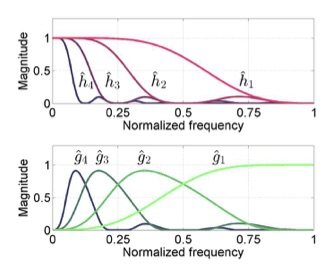
\includegraphics[width = 0.7 \textwidth]{./Diagrams/magnitude_response.jpg}
\caption{Frequency responses of the scaling and wavelet filters $h_j,g_j,j=1,\ldots,4$. Figure taken from \cite{LF-Shearlets} pp. 4}
\label{fig:magnitude_response}
\end{figure}

As it was presented for first time in \cite{Nonseparableshear}, the shear transform $S_{k2^{-j}}$, $j\in\mathbb{N}$, $k\in\mathbb{Z}$ does not preserve the regular grit $\mathbb{Z}^2$, therefore its digitalization is non-trivial. To tackle this issue, one needs to refine the $\mathbb{Z}^2$ grid along the $x_1-axis$ by a factor $2^j$, then the new grid $2^{-j}\mathbb{Z}\times\mathbb{Z}$ is invariant under the $S_{k 2^{-j}}$ transform. 

\bigskip

For an arbitrary $r\in \ell^2(\mathbb{Z}^2)$, the shear transform $S_{k 2^{-j}}$ can be implemented as a digital filter

\begin{equation}
\label{eq:LFshearlets6}
S^d_{k 2^{-j}}(r)=((2^jr_{\uparrow 2^j}\ast_1\tau_j)(S_k\cdot)\ast_1\overline{\tau}_j)_{\downarrow 2^j}
\end{equation}

where $\tau_j$ is a digital low-pass filter with normalized cutoff frequency at $2^-j$. 

\bigskip

Using the Equations~\ref{eq:LFshearlets3},~\ref{eq:LFshearlets4},~\ref{eq:LFshearlets5} and~\ref{eq:LFshearlets6} and the proper choice of $c_j$ it can be shown that the digital filter corresponding to $\psi_{j,k,m}$ is given by

$$
\psi_{j,k}^d=(S^d_{k2^{-(j+1)}}(p_j\ast g_{J-j}\otimes h_{J+1}))(m).
$$

A digital filter corresponding to separable elements of the transform $\phi_m$ related to the scaling function, is given by $\phi^d=(h_J\otimes h_J)(m)$. Then, the discrete shearlet transform associated with the set of elements $\Psi(c;\psi)$ and corresponding to frequency plane region $C_{\psi}$ is defined as follows

$$
\mathcal{DST}_{j,k,m}(f_J)=(f_J\ast \overline{\psi_{j,k}^d})(m),
$$

where $f_J(n)$ for $n\in\mathbb{Z}^2$ are discrete samples of $f\in L^2(\mathbb{R}^2)$, $j=0,\ldots,J-1$, $|k|\leq 2^{j+1}$, $m\in\mathbb{Z}^2$.

\bigskip

To compute the inverse transform we need to construct the dual frame; in order to do that we first set

$$
\hat{\Psi}^d=|\hat{\phi}^d|^2+\sum_{j=0,\ldots,J-1}\sum_{|k|\leq 2^{j+1}}(|\hat{\psi}^d_{j,k}|^2+|\hat{\tilde{\psi}}_{j,k}^d|^2).
$$ 

The dueal shearlet filters are defined by

$$
\hat{\phi}^d=\frac{\hat{\phi}^d}{\hat{\Psi}^d}\textrm{,}\quad \hat{\gamma}^d_{j,k}=\frac{\hat{\psi}^d_{j,k}}{\hat{\Psi}^d}\textrm{,}\quad \hat{\tilde{\gamma}}^d_{j,k}=\frac{\hat{\tilde{\psi}}_{j,k}^d}{\hat{\Psi}^d}
$$

\begin{figure}[h!]
\centering
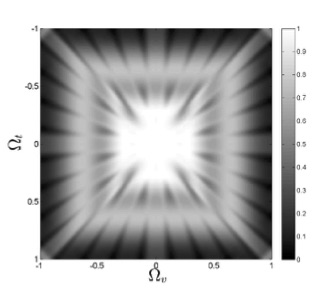
\includegraphics[width = 0.7 \textwidth]{./Diagrams/LFshearlets2e.jpg}
\caption{$\hat{\Psi}^d$ corresponding to constructed shearlet transform for $J=2$. Figure taken from \cite{LF-Shearlets} pp. 4}
\label{fig:LFshearlets2e}
\end{figure}

\begin{figure}[h!]
\centering
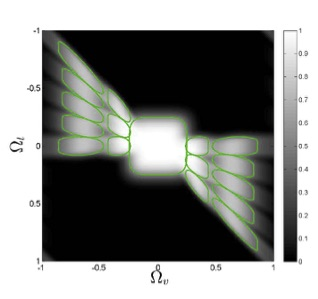
\includegraphics[width = 0.7 \textwidth]{./Diagrams/LFshearlets2f.jpg}
\caption{Frequency domain support of shearlet transform elements used in reconstruction. Figure taken from \cite{LF-Shearlets} pp. 4}
\label{fig:LFshearlets2f}
\end{figure}

One can see an illustration of the obtained system in the frequency plane $\hat{\Psi}^d$ for $J=2$ in Figure~\ref{fig:LFshearlets2e}. Finally, the reconstruction formula is given by

$$
f_J=(f_J\ast \overline{\phi}^d)\ast \phi^d+\sum_{j,k}(f_J\ast\overline{\psi}^d_{j,k})\ast \gamma^d_{j,k}+\sum_{j,k}(f_J\ast \overline{\tilde{\psi}}^d_{j,k})\tilde{\gamma}^d_{j,k}
$$

Following the methodology of \cite{LF-Shearlets} we will be interested only in the transform elements where the shearing has positibe sign, i.e. $0\leq k\leq 2^{j+1}$, the corresponding transform elements are ccovering the frequency domain region highlighted in Figure~\ref{fig:LFshearlets2f}. Then, we use the direct transform $S$ for discrete values $f_J$ and $j=0,\ldots J-1$, $k=0,\ldots, 2^{j+1}$, $m\in\mathbb{Z}^2$ defined as 

$$
S(f_J)=\{ c_{j,k}(m)=(f_J\ast \overline{\psi}_{j,k}^d)(m),c_0(m)=(f_J\ast \overline{\phi}^d)(m)\}.
$$

The inverse transform $S^*$ is then given by

$$
S^*(\{c_{j,k},c_0\})=\sum_{\begin{matrix}j=0,\ldots,J-1\\k=0,\ldots,2^{j+1}\end{matrix}}(c\ast \gamma_{j,k}^d)(m)+(c_0\ast\phi^d)(m).
$$

In the case of the Shearlet Transform implementation that we used for this thesis (Shearlab.jl) the $0$-Shearlet transform can be perform by choosing for each scale $j$ the number of shearings to be such that $|k|\leq 2^{j+1}$.

\bigskip

As a final remark for this section it is worth to mention that the $0$-Shearlet system is closely related to the Ridgelet Transform (see \cite{ridglet}), in the sense that both are computed by an inner product of an admissible generating function with different directional, scaling and translational parameters, where the scaling operation is performed in just one direction; the difference is that ridgelets perform directional operation by rotating the elements instead of shearing.

\bigskip

We have now all the tools necessary to perform the light field reconstruction using the Epipolar Plane Images method with sparsely sampled EPIs; in the next chapter we will present the minimization method used to perform such reconstruction as well as the results obtained numerically and the comparison with other light field reconstruction methods using different softwares and procedures. 

\chapter{Inpainting Sparse Sampled Epipolar-plane and Computing Depth Map}
\label{chap:Inpainting_sparse}

We just presented in Subsection~\ref{sec:shearlet_parseval_inpainting} a general framework for image inpainting using Parseval Frames and we also presented the comparison of general Shearlet Parseval Frames (which include Universal Shearlets, $\alpha$-Shearlets and Cone Adapted Shearlets) and Wavelet Parseval Frames in the task of inpainting a line-distribution singularity, having the conclusion that Shearlets present a faster convergence in the inpainting algorithm, this due its directional sensitivity.

\bigskip

We also presented in Subsection~\ref{sec:0-Shearlets} the particular case of Universal Shearlets with scaling sequence given by the parameters $\alpha_j=-2/j$, which generates a Parseval frame that is a good choice for the representation of singularities distributed over straight lines, and therefore is a good option for inpainting Epipolar Plane Images that are formed by linear structures.

\bigskip

In this chapter we will present a particular algorithm that we used to inpaint EPIs related to sparse sampled light fields using $0$-Shearlets in the Julia implemenation of Shearlab (Shearlab.jl) which is called Iterative Hard Thresholding; we will also present the results on the inpainting of a particular data set (the Church Data set already mentioned in Chapter 2). 

\bigskip

Using the inpainted EPIs we will present a line detection algorithm called Hough Line Transform that allows us to get the slopes of the lines related to different features in in the EPIs and therefore let us compute the depth map of the scene concluding the light field reconstruction task that we were looking for in this thesis. 

\section{Iterative thresholding algorithm for EPIs inpainting using $0$-Shearlets}

To formulate the light field reconstruction algorithm in discrete domain we will assume that that the starting coarse set of views is a downsampled version of the unknown densely sampled light field we are trying to reconstruct. The uniformly distributed cameras imply the possibility of estimating a common upper bound of disparities between consecutive views that we will call $d_{\text{max}}$; as we saw in Subsection~\ref{sec:phys_setup_sampling_rate} for densely sampled EPI's one need to ensure maximum 1 pixel disparity between nearby views (this in order to avoid aliasing and other artifacts), this representing minimum sampling rate law similar to Nyquist-Shannon sampling theorem. The given sparse set of views are regarded as taken at each $d_{max}=\lceil d_{max}\rceil$-th view of a densely sampled Light Field. 

\bigskip


As a very illustrative example one refers to the Figure~\ref{fig:sparse_EPI} where we have an EPI representation of four views with 16 pix disparity; we also established in Subsection~\ref{sec:phys_setup_sampling_rate} that it is sufficient to compute the slope of the lines representing certain scene points in the Epipolar plane images to know the relative depth in the scene of the correspondent feature point, this using the equation~\ref{eq:C2S5E4}; for that we will need to be able to see clear straight lines in the EPIs.

\bigskip

On Figure~\ref{fig:sparse_EPI} (a) one can see an sparse sampled Epipolar Plane Image, where the lines are not distinguishable; on Figure~\ref{fig:sparse_EPI}(b) when we separate the layers of the sparse sampled Epipolar Plane Image with 16px of disparity between the consecutive views the lines start to form; and finally the lines are clear in Figure~\ref{fig:sparse_EPI}(c), that represents the correspondent densely sampled Epipolar Plane Image which we want to recover by inpainting the sparse version. 

\bigskip

To proceed with the mathematics of the optimization problem that performs the inpainting, we will assume that the densely sampled EPI is a square image denoted by $y^*\in \mathbb{R}^{N\times N}$ where $N=md_{max}$ and $m$ is a number of avialable views. Given the samples $y\in\mathbb{R}^{N\times N}$ of the dense $y^*$ obtained by 

\begin{equation}
\label{eq:lfshearlets7}
y(i,j)=M(i,j)y^*(i,j)
\end{equation}

where $M\in\mathbb{R}^{N\times N}$ is a measuring matrix from which one can get the mask for the inpainting problem, such that $M(kd_{max},\cdot)=1$ for $k=1,\ldots,m$ and $0$ elsewhere. The measurements $y$ form an incomplete EPI where only rows from the available images are presented, while everywhere else EPI values are $0$. We can rewrite the Equation~\ref{eq:lfshearlets7} as $y=Hy^*$ by lexicographically reordering the variables $y,y^*\in \mathbb{R}^{N^2}$, $H\in\mathbb{R}^{N^2\times N^2}$. 

\bigskip 

Let $\mathcal{SH}(\psi,\phi,(-2/j)_j\in\mathbb{Z})$ be the system of $0$-Shearlets, defined in the Subsection~\ref{sec:0-Shearlets}; in addition let $S:\mathbb{R}^{N\times N}\longrightarrow \mathbb{R}^{N\times N\times\eta}$ and $S^*: \mathbb{R}^{N\times N\times\eta}\longrightarrow \mathbb{R}^{N\times N}$ the analysis and synthesis operator related to the $0$-Shearlet system defined in equations~\ref{eq:0analysis} and~\ref{eq:0synthesis}, where $\eta$ is the number of all translation invariant transform elements.

\bigskip 

The reconstruction problem of $y^*$ defined by the sampling matrix $M$ and the measurements $y$ can be cast as an inpainting problem following the framework of Subsection~\ref{sec:shearlet_parseval_inpainting} given by,

\begin{equation}
\label{eq:lfshearlets8}
x^*=\underset{x\in\mathbb{R}^{N\times N}}{\textrm{argmin}}||S(x)||_1,\quad \textrm{subject to}\quad y=Mx
\end{equation}

\bigskip

The algorithm that we will use to solve the optimization problem will make use of iterative procedures applied in morphological component analysis approaches, which have been originally proposed for decomposing images into piecewise-smooth and texture parts (see \cite{morph} and \cite{mcalab}), this algorithm is also known as Iterative Hard Thresholding. Following the approach of Vagharshakyan \cite{LF-Shearlets}, we aim to recunstruct the EPI $y^*$ by performing regularization in the shearlet transform domain by its sparsifying properties for cartoon-like functions. 

\bigskip

The solution is sought in the form of the algorithm~\ref{alg:lfshearlets1}. 

\begin{algorithm}[h!]
    \SetKwInOut{Input}{Input}
    \SetKwInOut{Output}{Output}
		\SetKwInOut{Compute}{Compute}

    \Input{Sparse EPI $y$, sampling matrix $M$, $\delta_{init}$,$\delta_{min}$, iterations}
		\Compute{$x_0:=0$;\\
						 $\delta_0:=\delta_{init}$;\\
						 $\lambda:=(\delta_{min})^{1/(iterations-1)}$;\\
						 $\Gamma_0 := \textrm{supp}(S(x_0))$;\\
					   $\beta_0 := S_{\Gamma_0}(y-Mx_0)$;\\
						 $\alpha_0 =\frac{||\beta_0||_2^2}{||MS^*(\beta_0)||_2^2}$;\\
						 \textbf{for} $n:=0$ \textbf{to} (iterations-1) \textbf{do}\\
							 \hspace{5mm} $x_{n+1}=S^*(T_{\delta_n}(S(x_n+\alpha_n(y-Mx_n))))$;\\
							 \hspace{5mm} $\Gamma_{n+1} := \textrm{supp}(S(x_{n+1}))$;\\
					     \hspace{5mm} $\beta_{n+1} := S_{\Gamma_{n+1}}(y-Mx_{n+1})$;\\
						 	 \hspace{5mm} $\alpha_{n+1}: =\frac{||\beta_{n+1}||_2^2}{||MS^*(\beta_{n+1})||}$;\\
							 \hspace{5mm} $\delta_{n+1} :=\lambda\delta_n;$\\
							\textbf{end}}
    \Output{Inpainted EPI $x_{iterations}$}
    \caption{Inpainting via iterative hard thresholding}
		\label{alg:lfshearlets1}
\end{algorithm}

\bigskip

In the Algorithm~\ref{alg:lfshearlets1}, the operator $T_{\delta}$ is the hard thresholding operator given by:

$$
(T_{\delta}x)(k)=\begin{cases} x(k)\textrm{,}\quad |x(k)|\geq \delta \\ 0\textrm{,}\quad |x(k)|<\delta \end{cases}
$$

The thresholding level $\delta_n$ decreases with the iteration number linearly in the range $[\delta_{max},\delta_{min}]$. The sequence $x_n$ that converges to $x^*$ reaches a solution of the problem~\ref{eq:lfshearlets8}, we refer to Figure~\ref{fig:EPI_rec} for the complete pipeline of the reconstruction method.

\bigskip

Here $\alpha_n$ is an acceleration parameter; in the usual inpainting algorithms based on the Shearlet Transform the chosen parameter is $\alpha_n=1$ (see \cite{Analysisinpaint} and \cite{Shearlab}) but the convergence in this case is slow and can be accelerated by using $\alpha_n>1$. It is also not optimal to take alpha too high, since this can cause instability. One can see on Figure~\ref{fig:alpha_accel} that convergence speed increases when increasing fixed values $\alpha_n = \alpha$ up to some level where the algorithm starts to diverge.

\begin{figure}[h!]
\centering
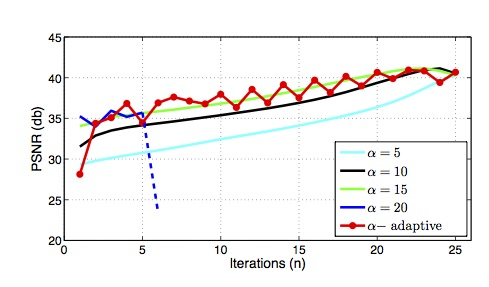
\includegraphics[width = 0.9 \textwidth]{./Diagrams/alpha_accel.jpg}
\caption{Reconstruction performance (expressed in terms of Peak Signal-to-Noise radio) dependence on acceleration coefficients $\alpha_n$, for contant value for all iterations $\alpha_n=\alpha$, increasing $\alpha$ brings accelerating convergence, but after some limit, the reconstruction starts to diverge ($\alpha = 20$). Figure taken from \cite{LF-Shearlets} pp. 7}
\label{fig:alpha_accel}
\end{figure}

The approach that we will use and is presented in Algorithm~\ref{alg:lfshearlets1} was proposed by T. Blumensath and M. Davies in 2010 in their article "Normalised Iterative Hard Thresholding; guaranteed stability and performance" \cite{hard-thresholding}. This algorithm applies an iteration-adaptative selection of the parameter given by

$$
\alpha_n=\frac{||\beta_n||_2^2}{||MS^*(\beta_n)||_2^2}
$$

where $\beta_n=S_{\Gamma_n}(y-Mx_n)$ and $S_{\Gamma_n}$ is the shearlet transform decomposition only for coefficients from $\Gamma_n=\textrm{supp}(S(x_n))$; it is important to be noticed that $||\cdot||_2$ is the Eucledian norm in the associated $N^2\eta$-dimensional Eucledian space of $\mathbb{R}^{N\times N\times \eta}$ with elements arranged in lexicographic order. The convergence rate of the adaptative selection is also illustrated in Figure~\ref{fig:alpha_accel} and one can see that the adaptation provides high convergence speed and stable reconstruction we refer to the original paper \cite{hard-thresholding} for a more detailed analysis of the convergence and stability conditions, which for our case are fulfilled using the fact that the $0$-Shearlets system form a Parseval Frame. 

\bigskip

As we discurssed in Subsection~\ref{sec:0-Shearlets} we are not obligated to use all the general shearlet transform atoms, instead we favor the use of atoms which are associated with valid directions in EPI; the support of those atomis is illustrated in Figure~\ref{fig:LFshearlets2f}. The scales of the shearlet transform are constructed in dyadic manner, therefore we are choosing $J = \lceil log_2 d_{max}\rceil$ number of scales. In order to perform this programatically using the software Shearlab.jl in every scale we choose $2^{j+1}+1$ shears ($j=0,\ldots, J-1$) to cover the region.

\bigskip

Finally, in the following subsections we will present the resulting inpainted EPIs of the Church data set, as well as the technique that we use to detect lines in the inpainted EPIs and finally compute the depth map. 

\section{Results of sparse EPIs inpaiting}

In order to give the full picture of the EPIs inpainting algorithm implementation and results, we will present the set of ideas that made us take some decisions in the way to design the implementation of the inpainting algorithm.

\bigskip 

As we presented to Section~\ref{sec:Sparse-acquisition} the data set that we used was a series of pictures of a Church, given by the research group of Professor Markus Gross in the Disney Research Center. The data set has 100 different views of the scene, we present in~\ref{fig:first_church},~\ref{fig:second_church} and~\ref{fig:third_church} the 1st, 55th and 100th views of the data set.

\begin{figure}[h!]
\centering
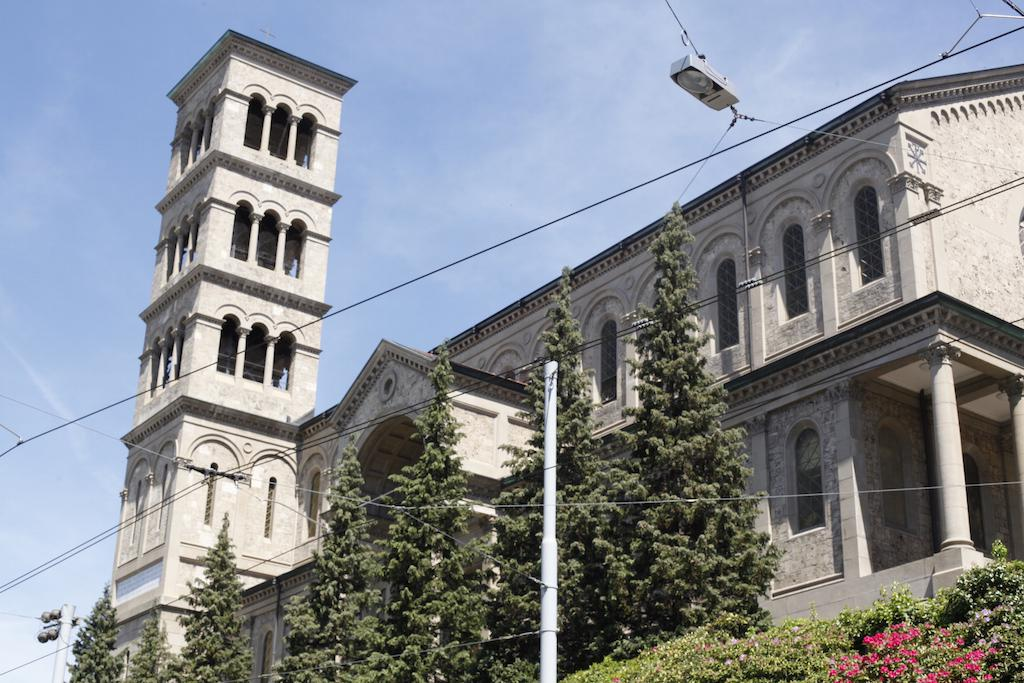
\includegraphics[width = 0.7 \textwidth]{./Diagrams/results/data_set/church_image-raw_0000_lowres.jpg}
\caption{1st picture of the Church Data Set}
\label{fig:first_church}
\end{figure}

\begin{figure}[h!]
\centering
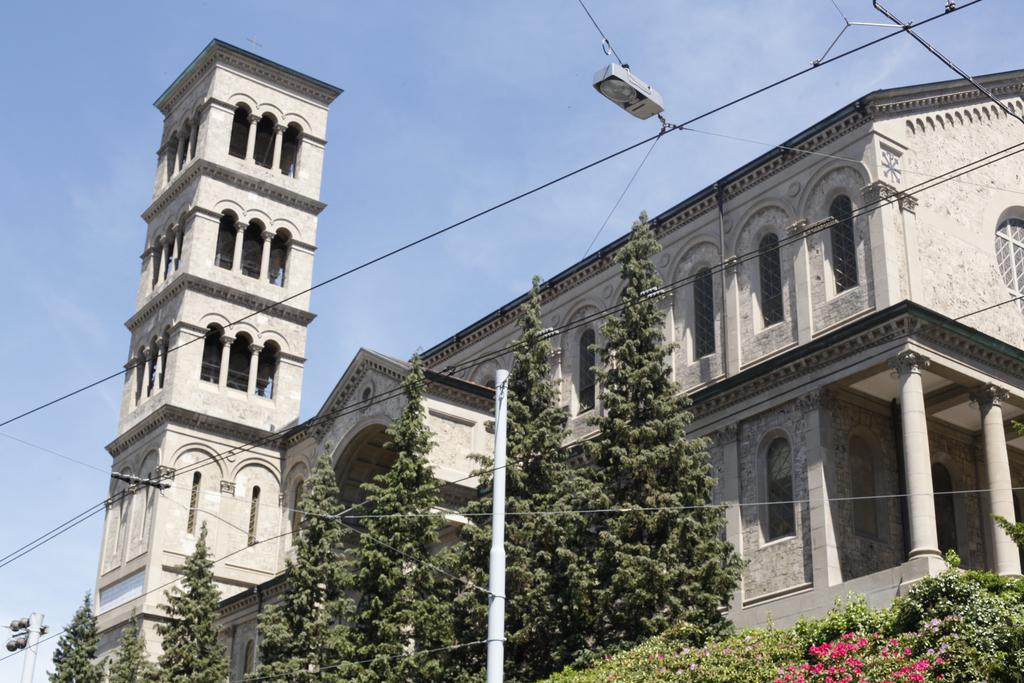
\includegraphics[width = 0.7 \textwidth]{./Diagrams/results/data_set/church_image-raw_0055_lowres.jpg}
\caption{55th picture of the Church Data Set}
\label{fig:second_church}
\end{figure}

\begin{figure}[h!]
\centering
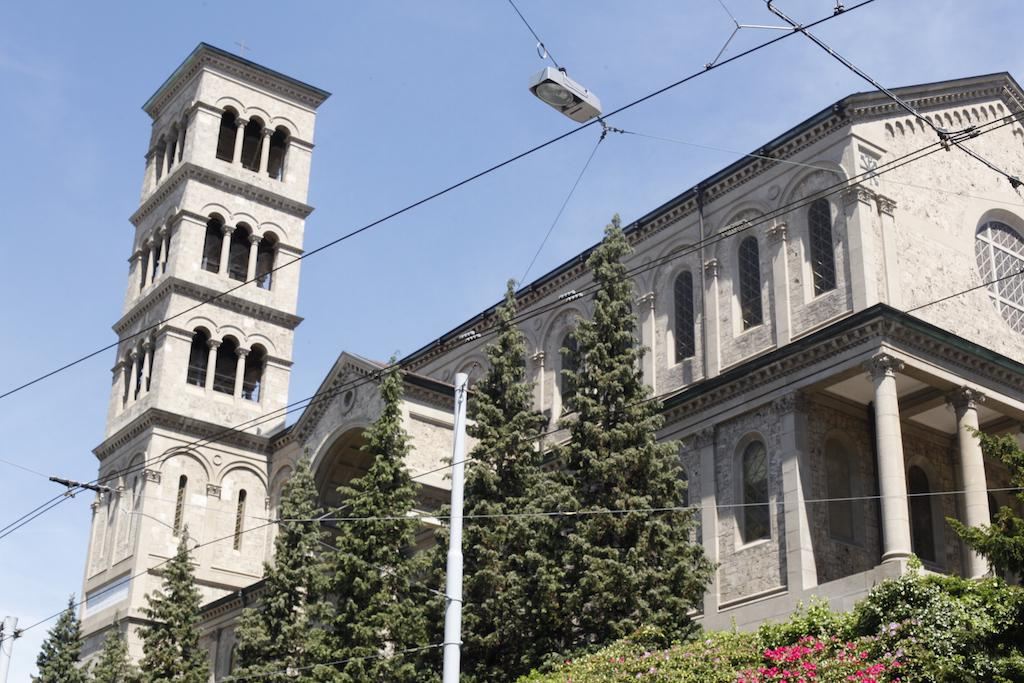
\includegraphics[width = 0.7 \textwidth]{./Diagrams/results/data_set/church_image-raw_0100_lowres.jpg}
\caption{100th picture of the Church Data Set}
\label{fig:third_church}
\end{figure}


\bigskip

\begin{itemize}

\item \textbf{First step (Track Points):} The first step in the implementation was the design the code to track the points; in the Subsection~\ref{sec:proc_track} we presented the followed algorithm (Lucas-Kanade method with Shi-Tomasi corner detector) whose implementation using OpenCV Python's API is presented in Appendix~\ref{sec:Appendix_A} with the results were stored in a data frame that one can find in the repository of this thesis (\url{https://github.com/arsenal9971/MThesis/blob/master/Code_notebooks/church_tracking.csv}) and are presented in Figure~\ref{fig:track_points_church}.

\bigskip

\item \textbf{Second Step (Paint sparse EPIs):}Once we had the data of the tracked points we proceed to paint the EPIs related to fixed $y$-positions in the scenes, for this task we used the julia code presented in Appendix~\ref{sec:Appendix_B}, where we used horizontal strips of width $2\epsilon=16.0$ pixels to captures tracked points in the scene at different fixed $y$ positions and follow them along the different views, we also used the same data set to paint the corresponding Sparse Views with a constant disparity between consecutive views $d_{max}=7px$; this maximum disparity was chosen by trying different disparities and pick the best one in terms of the painting speed (the greater the disparity, the less time it takes to paint the sparse EPIs) and the Shearlet-based inpainting performance using a fixed number of iterations (50) in the iterative thresholding algorithm; where we measure the performance mostly in terms of how many lines of the original EPI are captured by our line detection algorithm that will be explained in the next subsection. One can see in Figure~\ref{fig:strip_disparity} the strip of points in the first image that were tracked to perform the benchmark to compute the best disparity parameter for our task; the Figure~\ref{fig:dense_disparity} is the associated densely sampled EPI and the associated sparsely sampled EPIs with different disparities $d_{max}$ are presented in Figure~\ref{fig:first_sparse_disparity},~\ref{fig:second_sparse_disparity},~\ref{fig:third_sparse_disparity} and~\ref{fig:fourth_sparse_disparity}. 

\bigskip

Finally on Figure~\ref{fig:benchmark_line} one can see the different running time obtained for different disparities (clearly the smaller the disparity, the more pictures you need to take and therefore the longest the running time); as we mentioned on Subsection~\ref{sec:proc_track} we used a Macbook Pro with OSX 10.10.5, 8GB of memory, 2.7 GHz Intel Core i5 Processor and Graphic Card Intel Iris Graphics 6100 with 1536 MB of graphic memory (relatively a low end computer system). One can find the whole set of strips, sparse and dense EPIs on \url{https://github.com/arsenal9971/MThesis/tree/master/Diagrams/results/EPIs}, the naming notation that we followed to identify them was \textbf{file\_name}=$y_0\_\epsilon\_t_{max}\_d_{max}\_tp\_f.png$ where $y_0$ is the $y$ position of the tracked points on the corresponding strip $\epsilon$ is half the width of the strip, $d_{max}$ is the used disparity for the corresponding sparse EPI, $tp$ is the number of tracked points in the strip and $f$ the number of features corresponding to the tracked points).

\bigskip

\begin{figure}[h!]
\centering
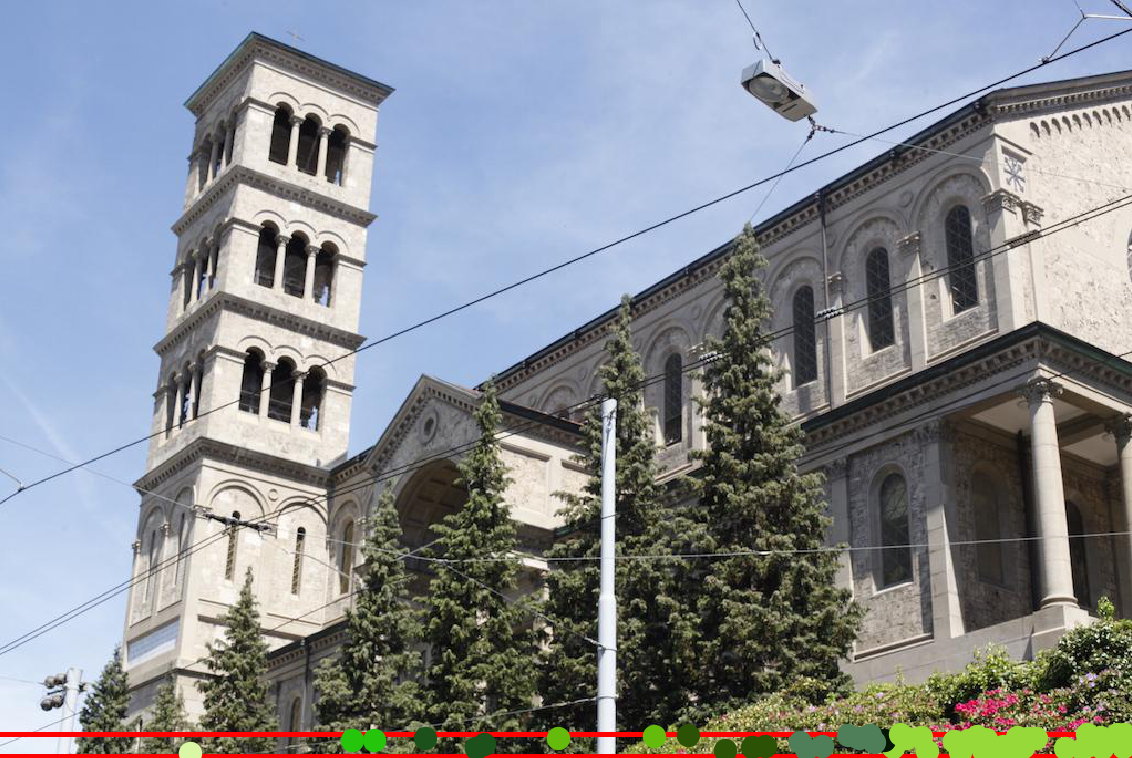
\includegraphics[width = 0.7 \textwidth]{./Diagrams/results/Disparity_benchmark/673_10_102_4_48_8_strip.png}
\caption{Strip of points of width $2\epsilon = 16.0$ px used for the benchmark to choose the disparity $d_{max}$}
\label{fig:strip_disparity}
\end{figure}

\begin{figure}[h!]
\centering
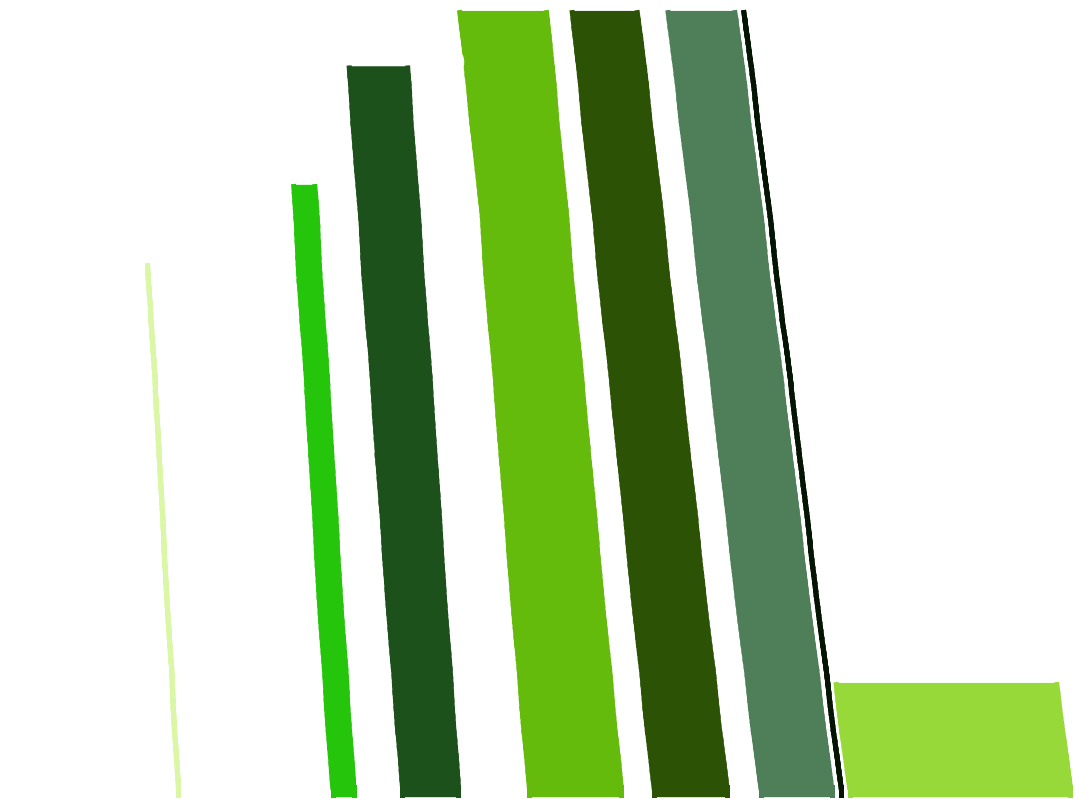
\includegraphics[width = 0.7 \textwidth]{./Diagrams/results/Disparity_benchmark/673_10_102_4_48_8_dense.png}
\caption{Densely sampled EPI associated to the points in the strip on Figure~\ref{fig:strip_disparity}}
\label{fig:dense_disparity}
\end{figure}

\begin{figure}[h!]
\centering
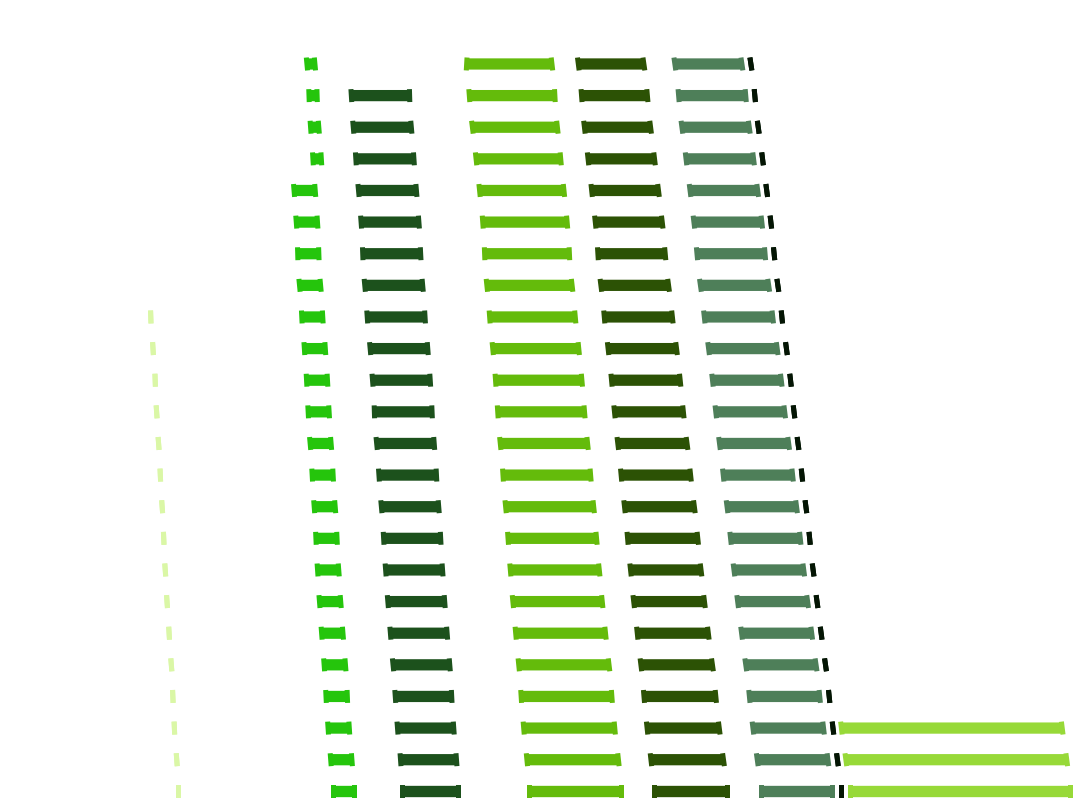
\includegraphics[width = 0.7 \textwidth]{./Diagrams/results/Disparity_benchmark/673_10_102_4_48_8_sparse.png}
\caption{Sparsely sampled EPI associated to the disparity $d_{max} = 4$ px}
\label{fig:first_sparse_disparity}
\end{figure}

\begin{figure}[h!]
\centering
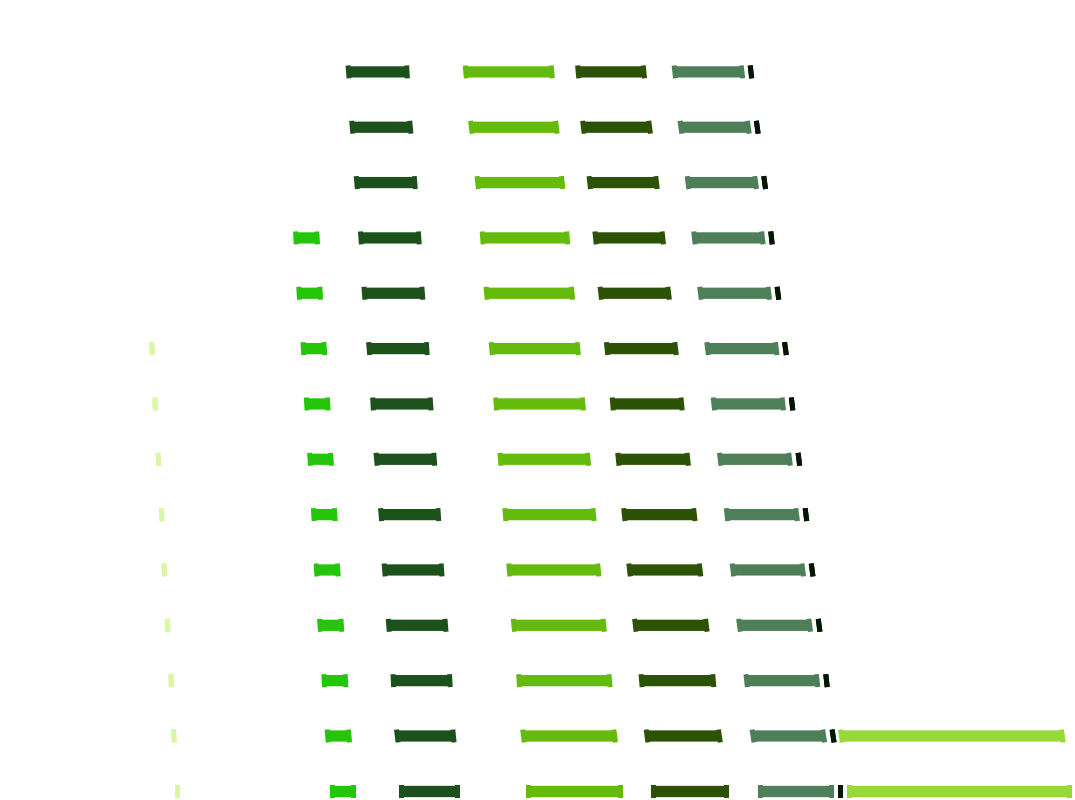
\includegraphics[width = 0.7 \textwidth]{./Diagrams/results/Disparity_benchmark/673_10_102_7_48_8_sparse.png}
\caption{Sparsely sampled EPI associated to the disparity $d_{max} = 7$ px}
\label{fig:second_sparse_disparity}
\end{figure}

\begin{figure}[h!]
\centering
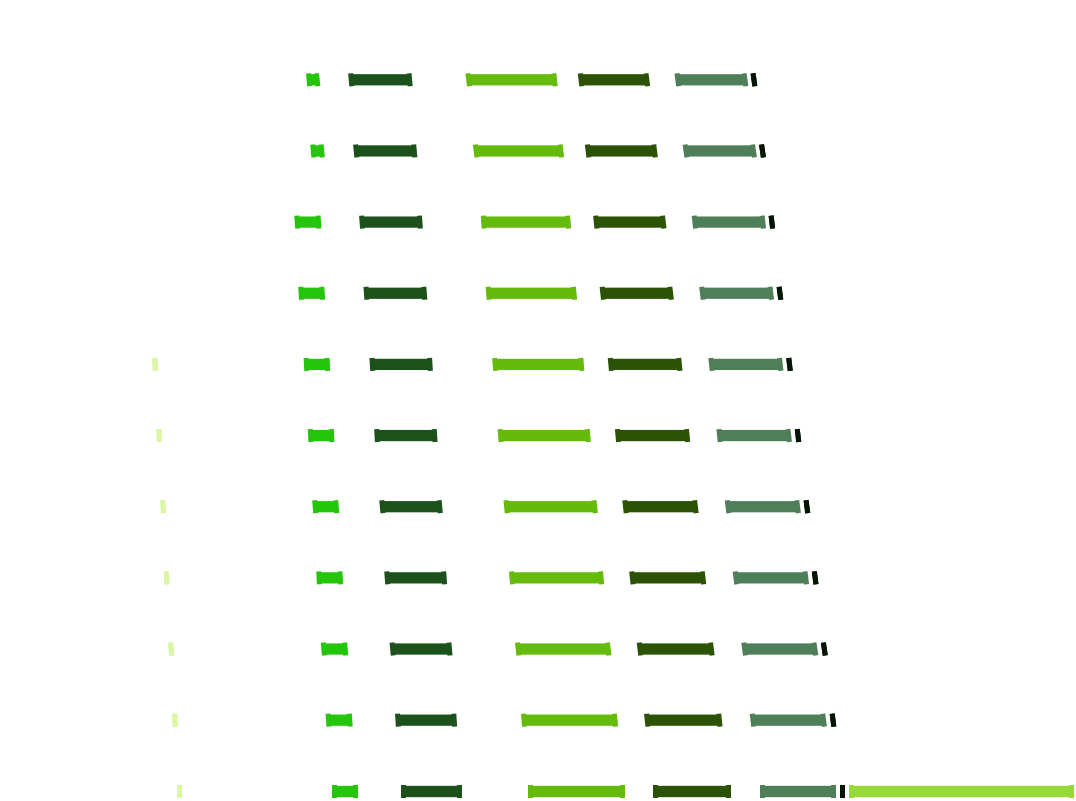
\includegraphics[width = 0.7 \textwidth]{./Diagrams/results/Disparity_benchmark/673_10_102_9_48_8_sparse.png}
\caption{Sparsely sampled EPI associated to the disparity $d_{max}=9$ px}
\label{fig:third_sparse_disparity}
\end{figure}

\begin{figure}[h!]
\centering
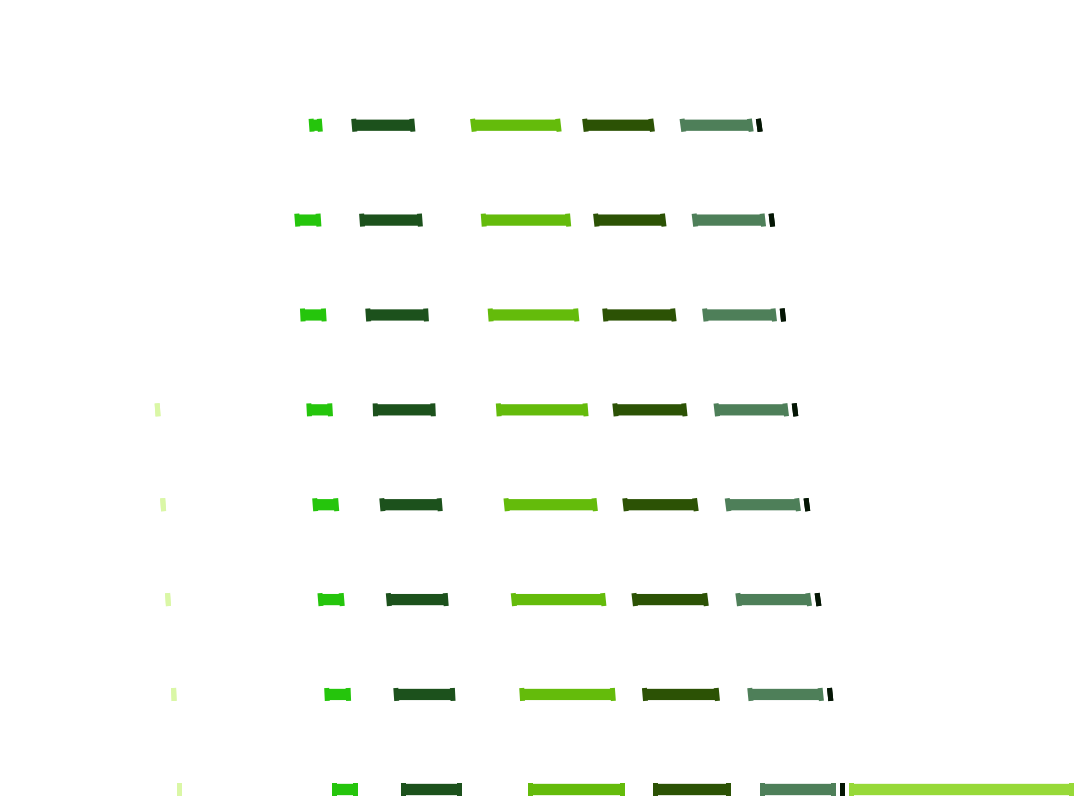
\includegraphics[width = 0.7 \textwidth]{./Diagrams/results/Disparity_benchmark/673_10_102_12_48_8_sparse.png}
\caption{Sparsely sampled EPI associated to the disparity $d_{max}=12$ px}
\label{fig:fourth_sparse_disparity}
\end{figure}

\begin{figure}[h!]
\centering
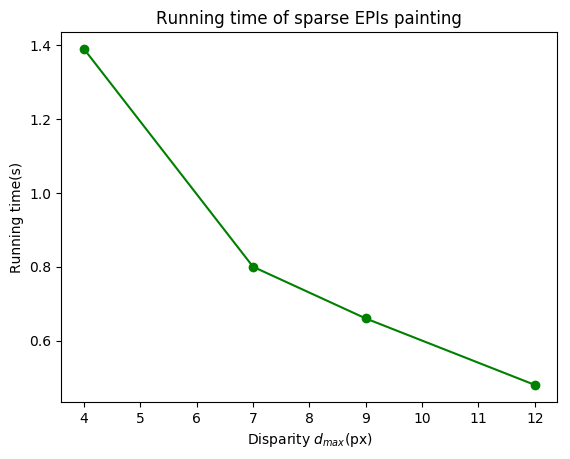
\includegraphics[width = 0.7 \textwidth]{./Diagrams/results/Disparity_benchmark/sparse_painting_benchmark.png}
\caption{Running time of painting of sparsely sampled EPIs with different disparities}
\label{fig:benchmark_line}
\end{figure}


\bigskip

One can also see in Figures~\ref{fig:first_lines_disparity},~\ref{fig:second_lines_disparity},~\ref{fig:third_lines_disparity} and~\ref{fig:fourth_lines_disparity} the lines detected in different inpainted EPIs corresponding to the same dense EPI, with different views disparity $d_{max}$, one can see that the important features are detected when $d_{max}=4$ and $d_{max}=7$ while when $d_{max}$ is bigger some lines are lost. 

\begin{figure}[h!]
\centering
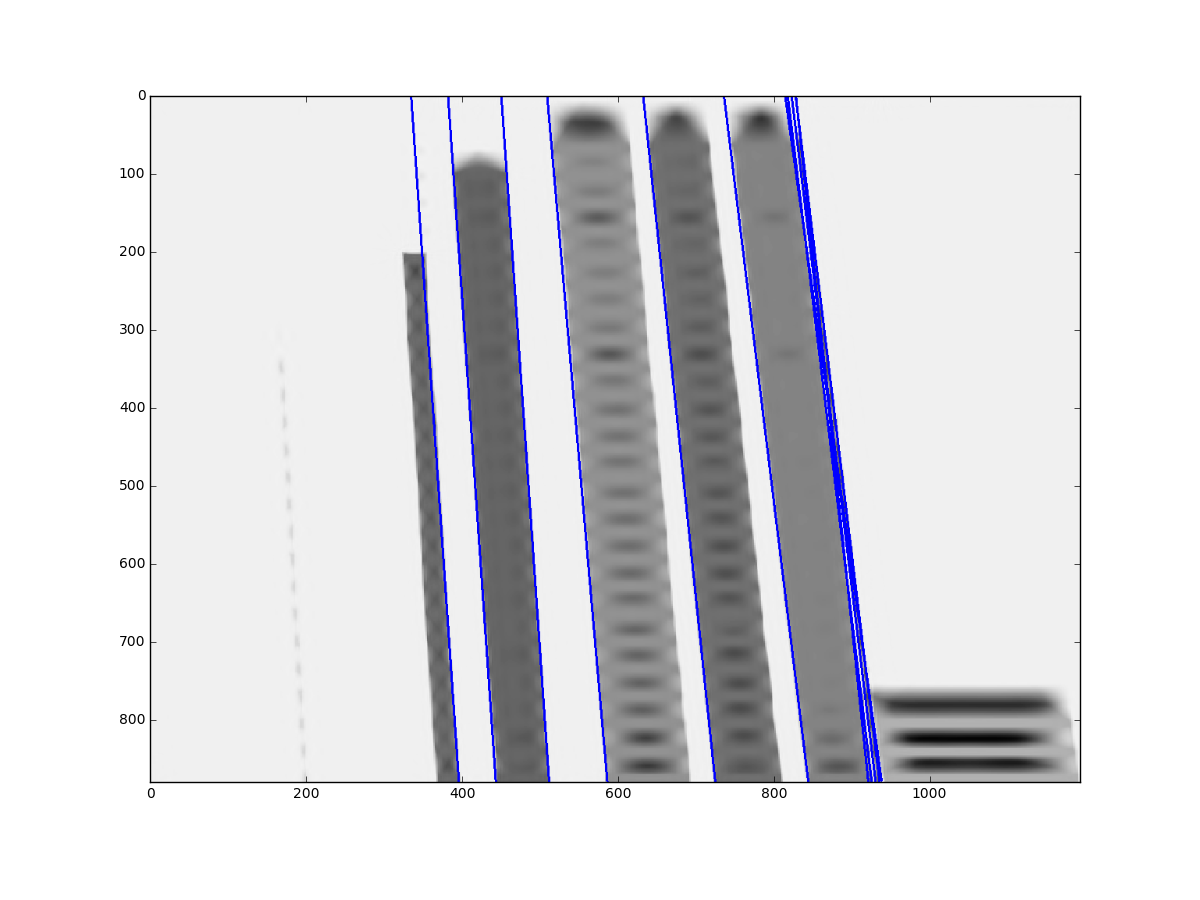
\includegraphics[width = 0.7 \textwidth]{./Diagrams/results/Disparity_benchmark/673_10_102_4_48_8_lines.png}
\caption{Lines detected in an inpainted using disparity $d_{max} = 4$ px}
\label{fig:first_lines_disparity}
\end{figure}

\begin{figure}[h!]
\centering
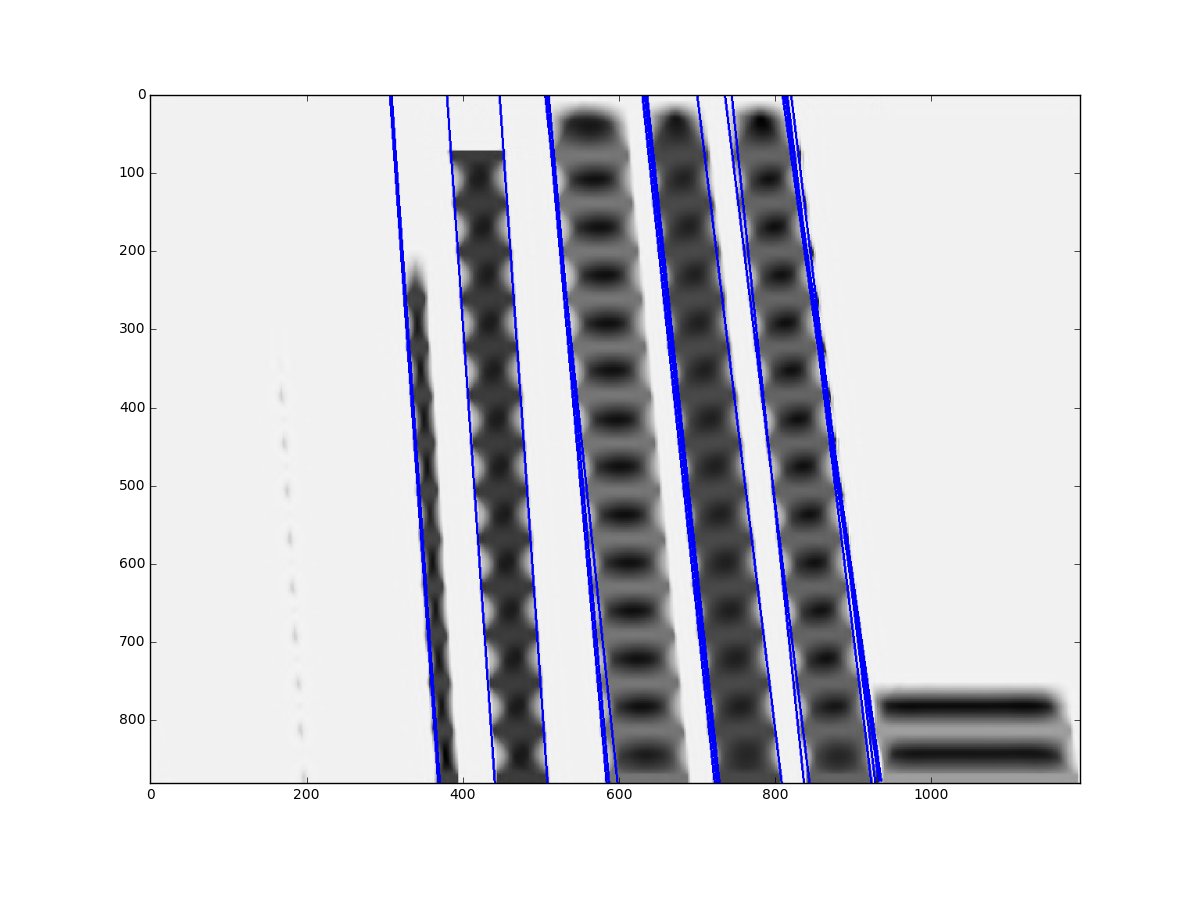
\includegraphics[width = 0.7 \textwidth]{./Diagrams/results/Disparity_benchmark/673_10_102_7_48_8_lines.png}
\caption{Lines detected in an inpainted using disparity $d_{max} = 7$ px}
\label{fig:second_lines_disparity}
\end{figure}

\begin{figure}[h!]
\centering
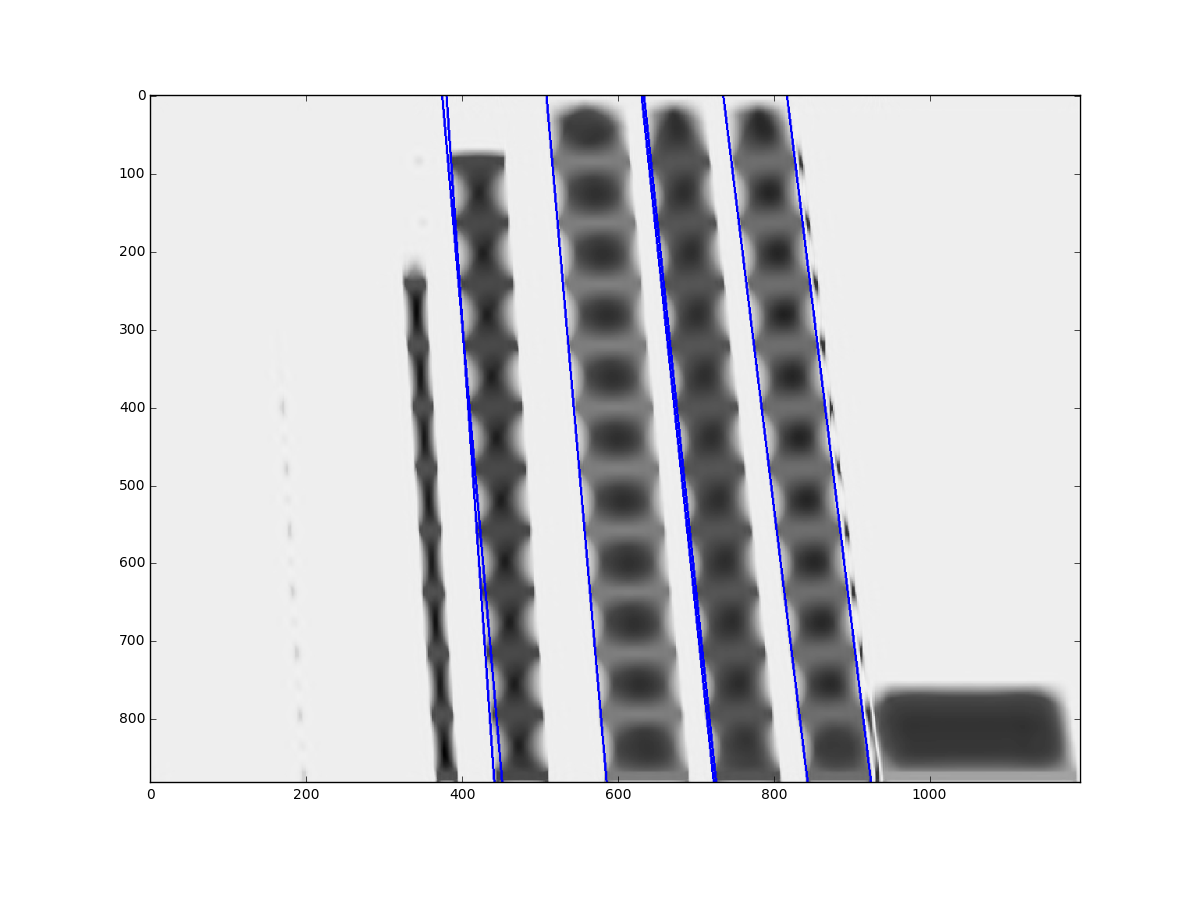
\includegraphics[width = 0.7 \textwidth]{./Diagrams/results/Disparity_benchmark/673_10_102_9_48_8_lines.png}
\caption{Lines detected in an inpainted using disparity $d_{max} = 9$ px}
\label{fig:third_lines_disparity}
\end{figure}

\begin{figure}[h!]
\centering
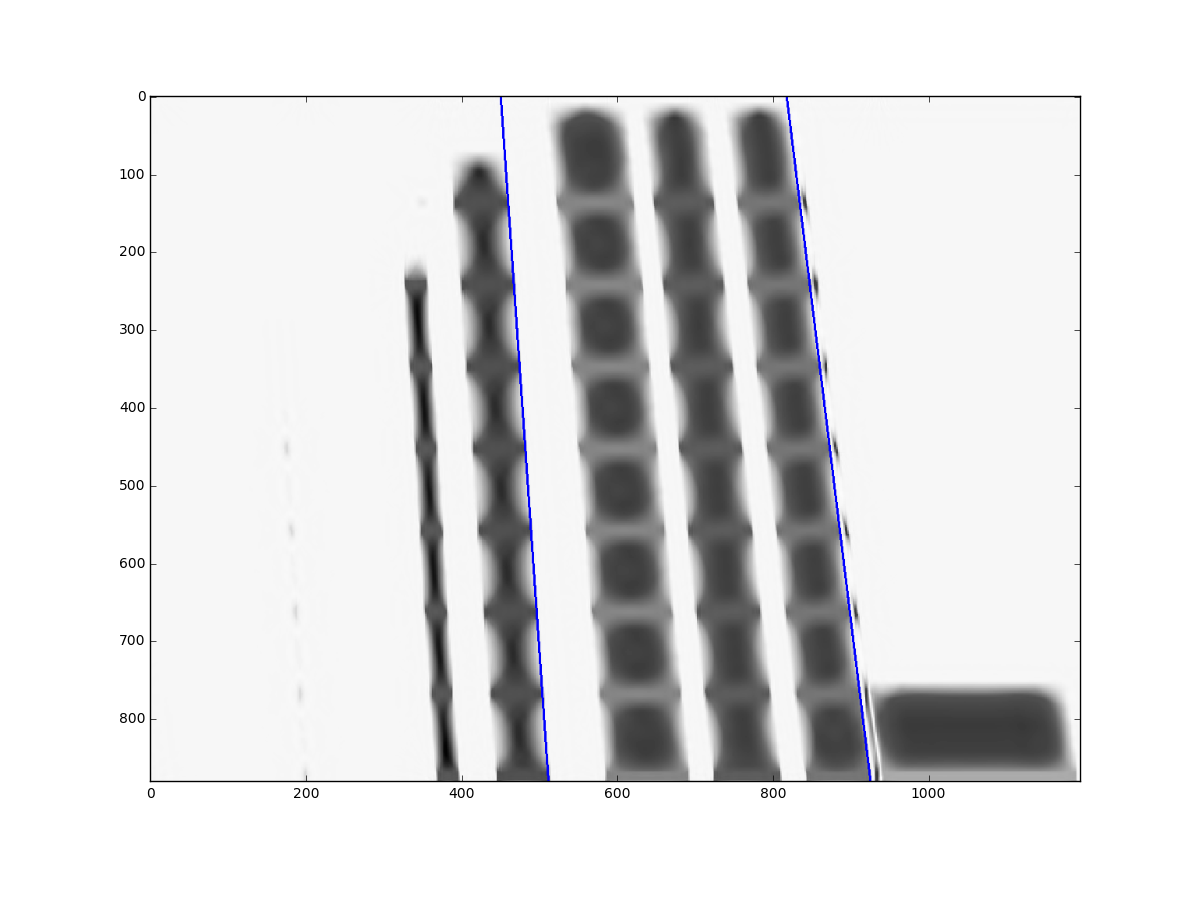
\includegraphics[width = 0.7 \textwidth]{./Diagrams/results/Disparity_benchmark/673_10_102_12_48_8_lines.png}
\caption{Lines detected in an inpainted using disparity $d_{max} = 12$ px}
\label{fig:fourth_lines_disparity}
\end{figure}

\begin{figure}[h!]
\centering
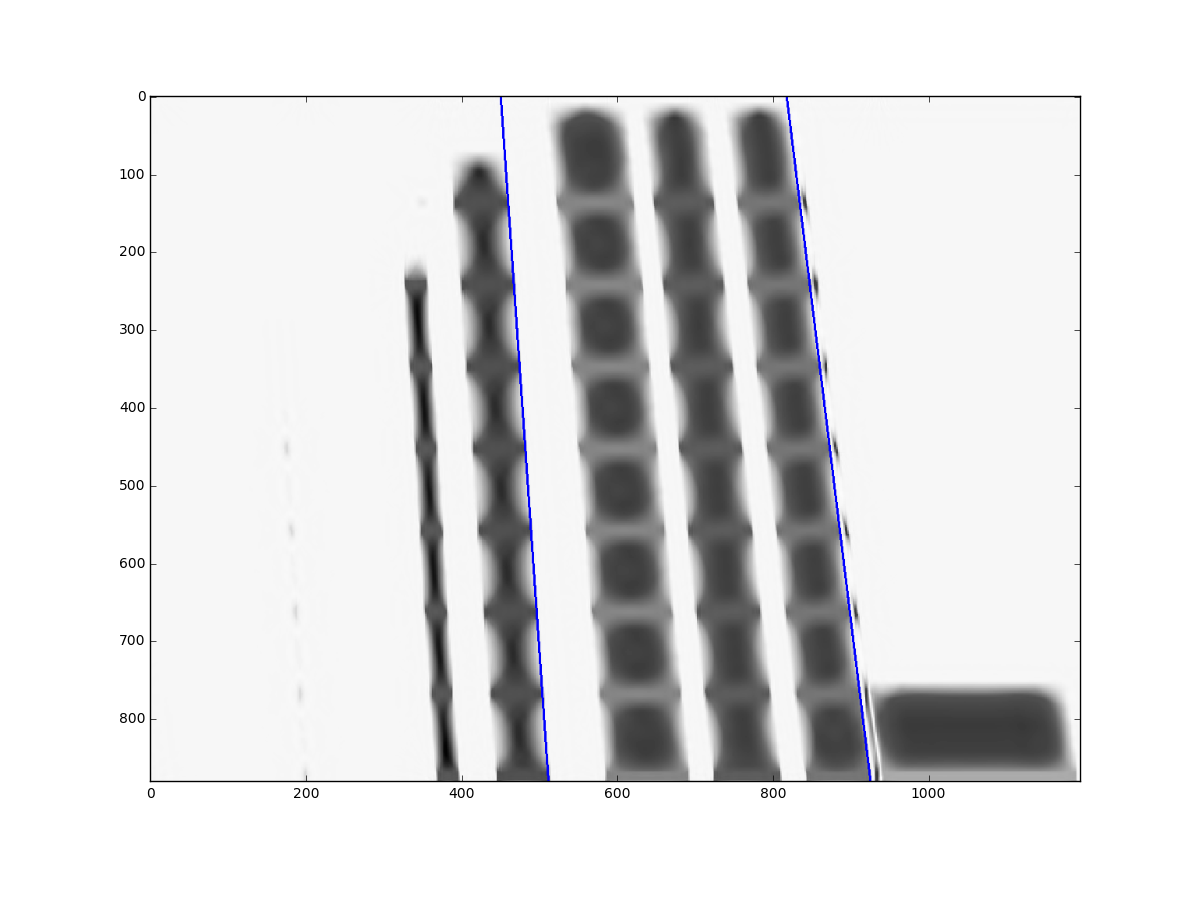
\includegraphics[width = 0.7 \textwidth]{./Diagrams/results/Disparity_benchmark/673_10_102_12_48_8_lines.png}
\caption{Lines detected in an inpainted using disparity $d_{max} = 12$ px}
\label{fig:fourth_lines_disparity}
\end{figure}

\begin{figure}[h!]
\centering
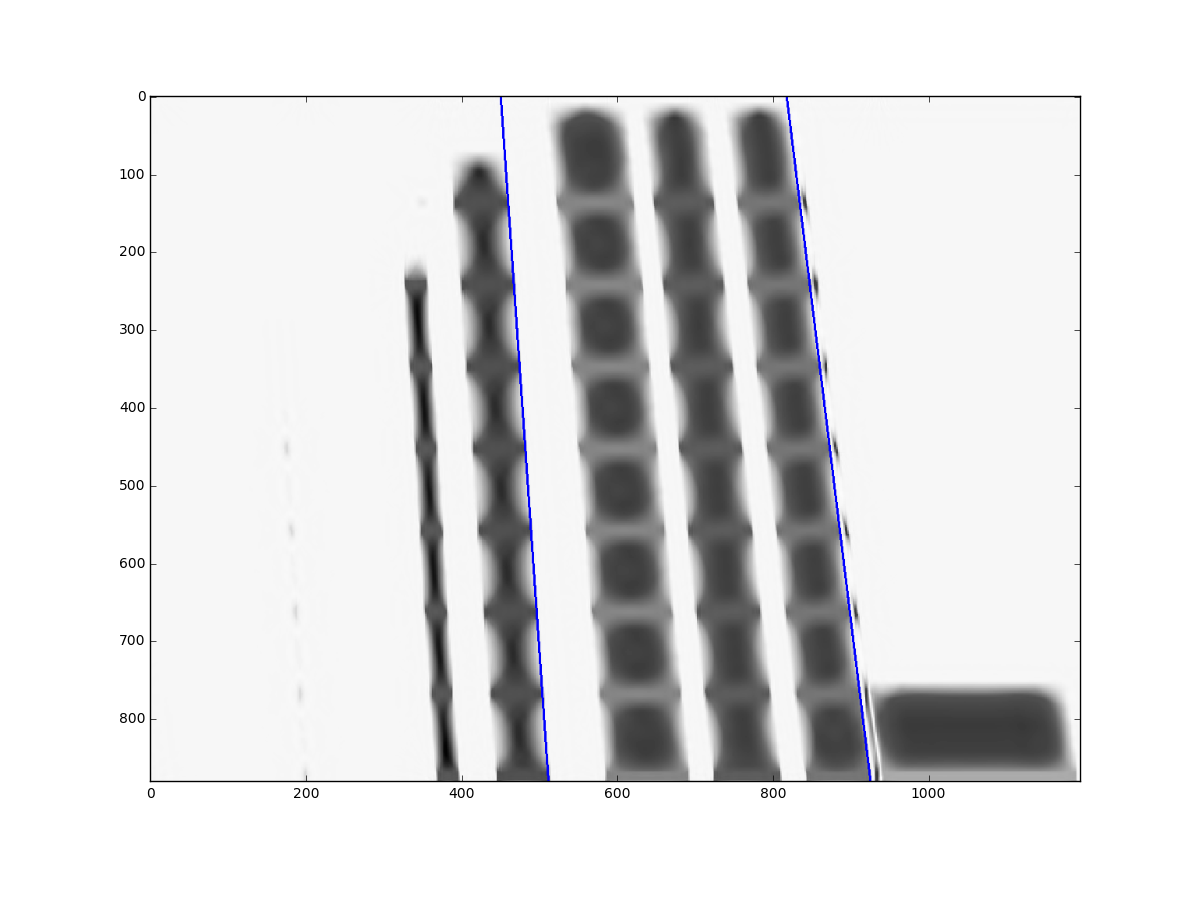
\includegraphics[width = 0.7 \textwidth]{./Diagrams/results/Disparity_benchmark/673_10_102_12_48_8_lines.png}
\caption{Lines detected in an inpainted using disparity $d_{max} = 12$ px}
\label{fig:fourth_lines_disparity}
\end{figure}

\item \textbf{Third step (Inpaint sparse EPIs):} After paint all the sparsely sampled EPIs corresponding to different horizontal strips of width $16.0$px whose union cover all the tracked points, we inpainted to recover a densely sampled EPIs and therefore we can finally compute the depth map by computing the slopes of the different lines in the EPIs. As we already mentioned on the last section, in order to perform the minimization problem associated with the inpainting algorithm we used iterative hard thresholding with a $0$-Shearlet system as sparsifying system whose code we can find on Appendix~\ref{sec:AppendixC} and was implemented using julia programming language with the libraries PyPlot.jl and Shearlab.jl. 

\bigskip

We choose some of the best EPIs (corresponding to strips that capture an important number of tracked points) to show here (see Figures~\ref{fig:strip1} to~\ref{fig:inpainted5}), but to compute the depth map we used all the inpainted EPIs that can be found on \url{https://github.com/arsenal9971/MThesis/tree/master/Diagrams/results/Inpainted} that follow the same naming notation as the dense EPIs, sparse EPIs and strips).

\bigskip

We are not looking here for high resolution light fields but for fast recoverable light fields so we imported in julia the sparse EPIs with a horizontal size of $n=512$ pixels, using the same computer system as already mentioned the inpainting of the EPIs with 50 iterations took 19.15 seconds when using a fixed acceleration parameter $\alpha = 1$, whereas it took 15.5 seconds when using a the adaptive acceleration parameter defined on Algorithm~\ref{alg:lfshearlets1}.

\begin{figure}[h!]
\centering
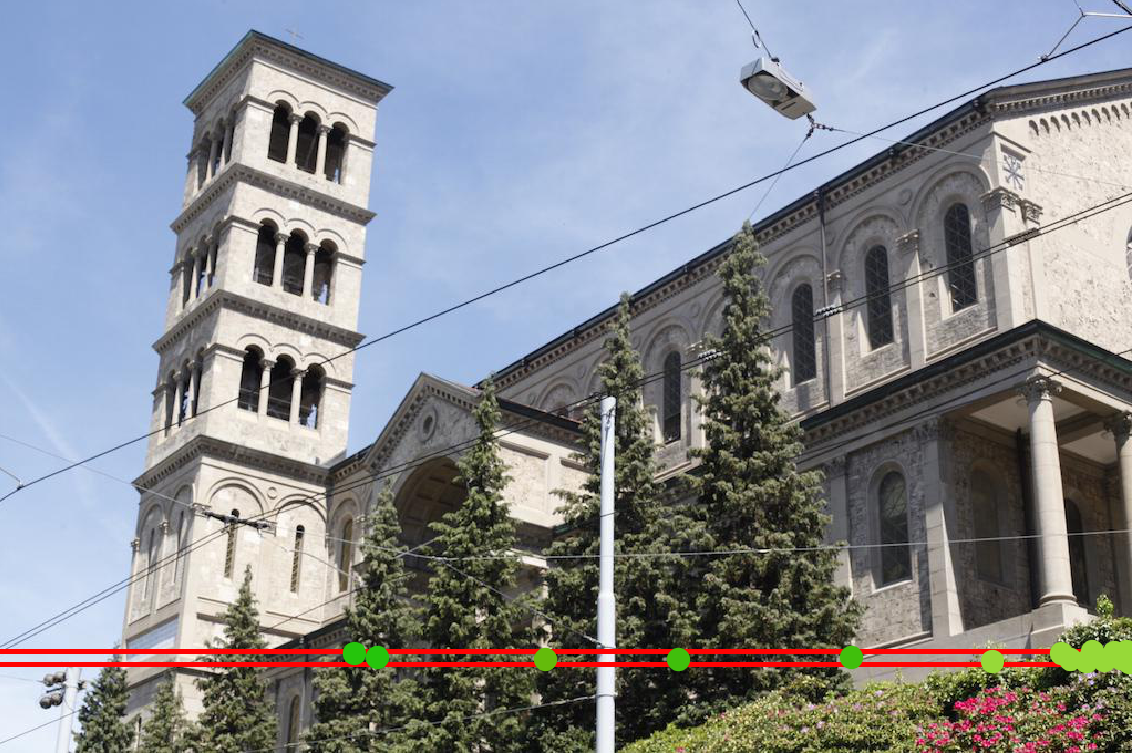
\includegraphics[width = 0.7 \textwidth]{./Diagrams/results/EPIs/392_8_102_7_15_4_strip.png}
\caption{Strip with tracked points}
\label{fig:strip1}
\end{figure}

\begin{figure}[h!]
\centering

\includegraphics[width = 0.7 \textwidth]{./Diagrams/results/EPIs/392_8_102_7_15_4_dense.png}
\caption{Dense EPI corresponding to the strip on Figure~\ref{fig:strip1}}
\label{fig:dense1}
\end{figure}

\begin{figure}[h!]
\centering
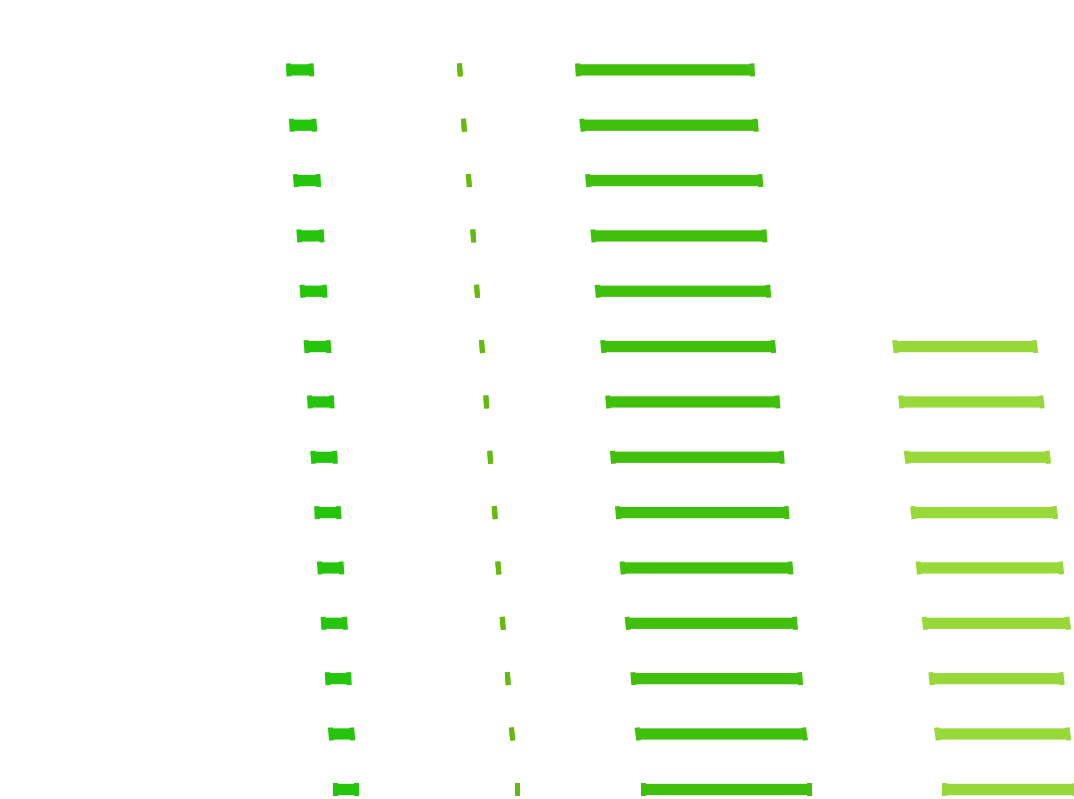
\includegraphics[width = 0.7 \textwidth]{./Diagrams/results/EPIs/392_8_102_7_15_4_sparse.png}
\caption{Sparse EPI corresponding to the strip on Figure~\ref{fig:strip1}}
\label{fig:sparse1}
\end{figure}

\begin{figure}[h!]
\centering
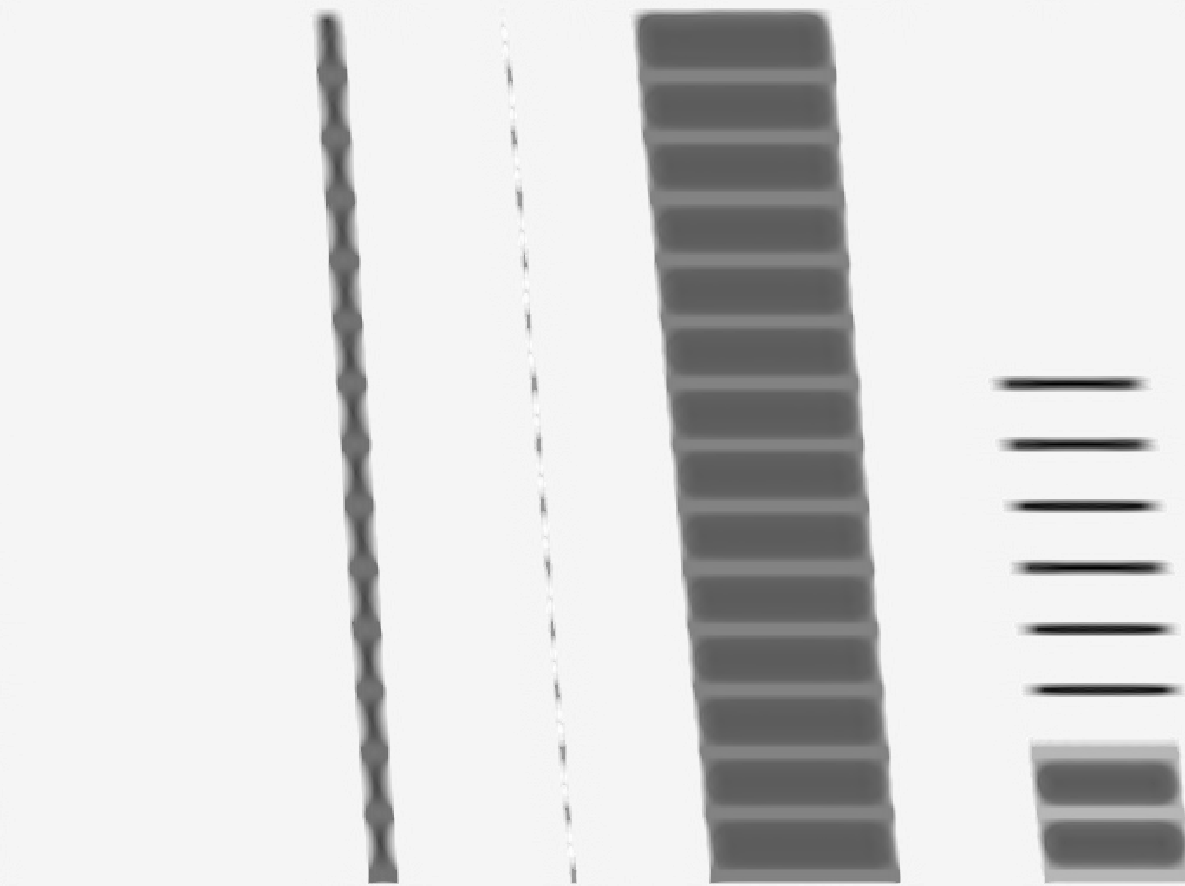
\includegraphics[width = 0.7 \textwidth]{./Diagrams/results/Inpainted/392_8_102_7_15_4_inpainted.png}
\caption{Inpainted EPI corresponding to the strip on Figure~\ref{fig:strip1}}
\label{fig:inpainted1}
\end{figure}


\begin{figure}[h!]
\centering
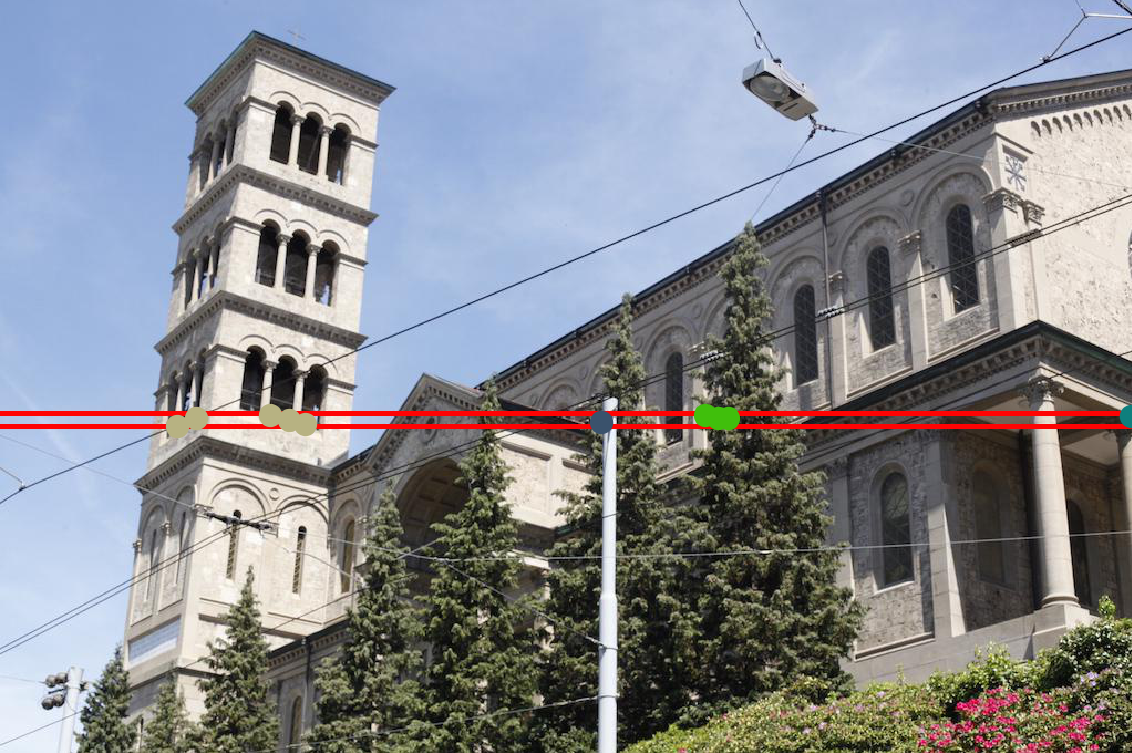
\includegraphics[width = 0.7 \textwidth]{./Diagrams/results/EPIs/424_8_102_7_10_4_strip.png}
\caption{Strip with tracked points}
\label{fig:strip2}
\end{figure}

\begin{figure}[h!]
\centering
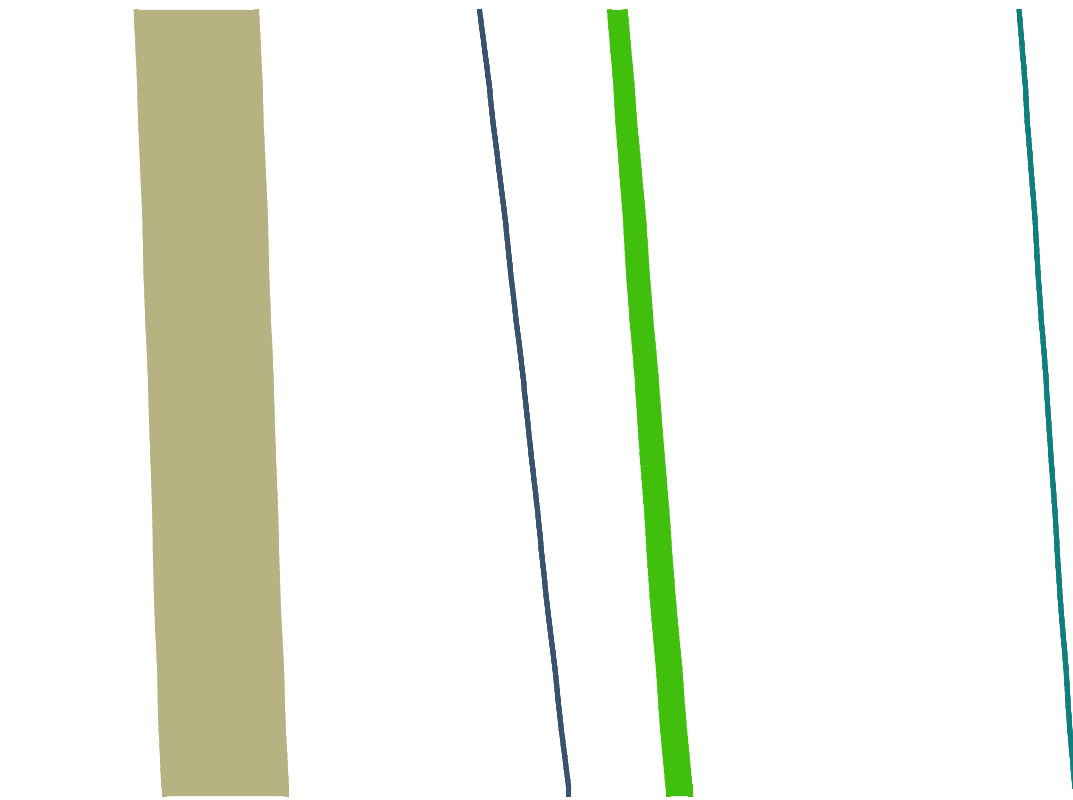
\includegraphics[width = 0.7 \textwidth]{./Diagrams/results/EPIs/424_8_102_7_10_4_dense.png}
\caption{Dense EPI corresponding to the strip on Figure~\ref{fig:strip2}}
\label{fig:dense2}
\end{figure}

\begin{figure}[h!]
\centering
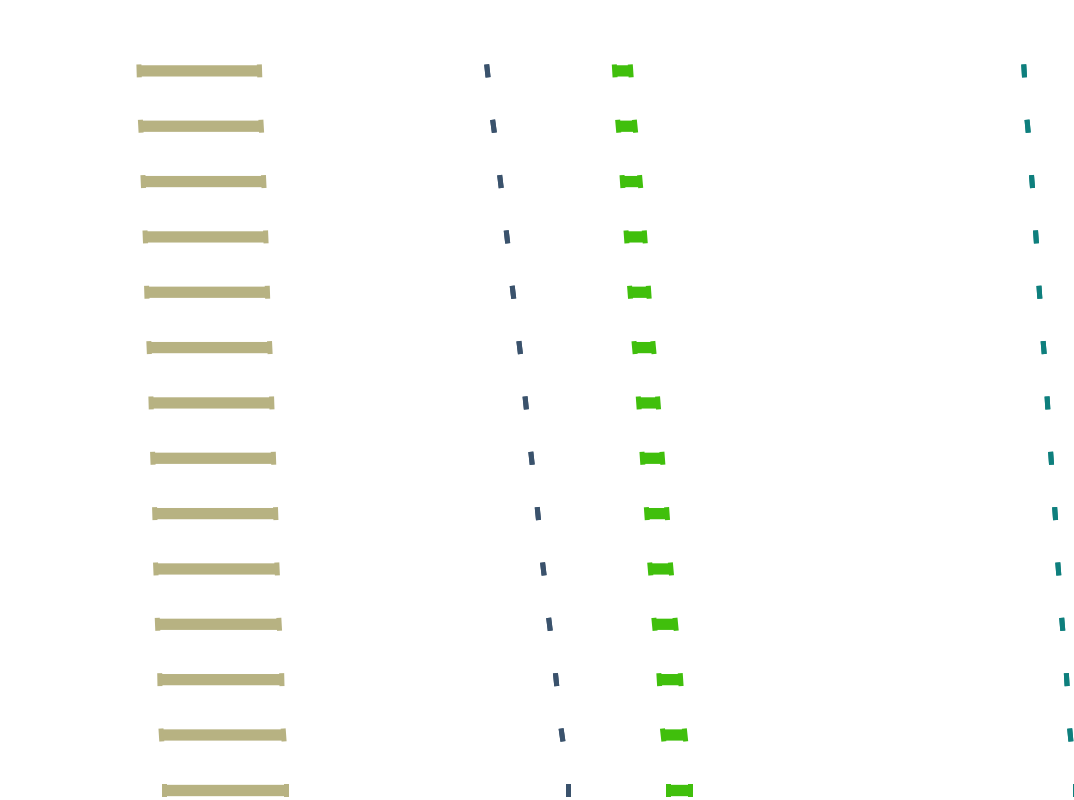
\includegraphics[width = 0.7 \textwidth]{./Diagrams/results/EPIs/424_8_102_7_10_4_sparse.png}
\caption{Sparse EPI corresponding to the strip on Figure~\ref{fig:strip2}}
\label{fig:sparse2}
\end{figure}

\begin{figure}[h!]
\centering
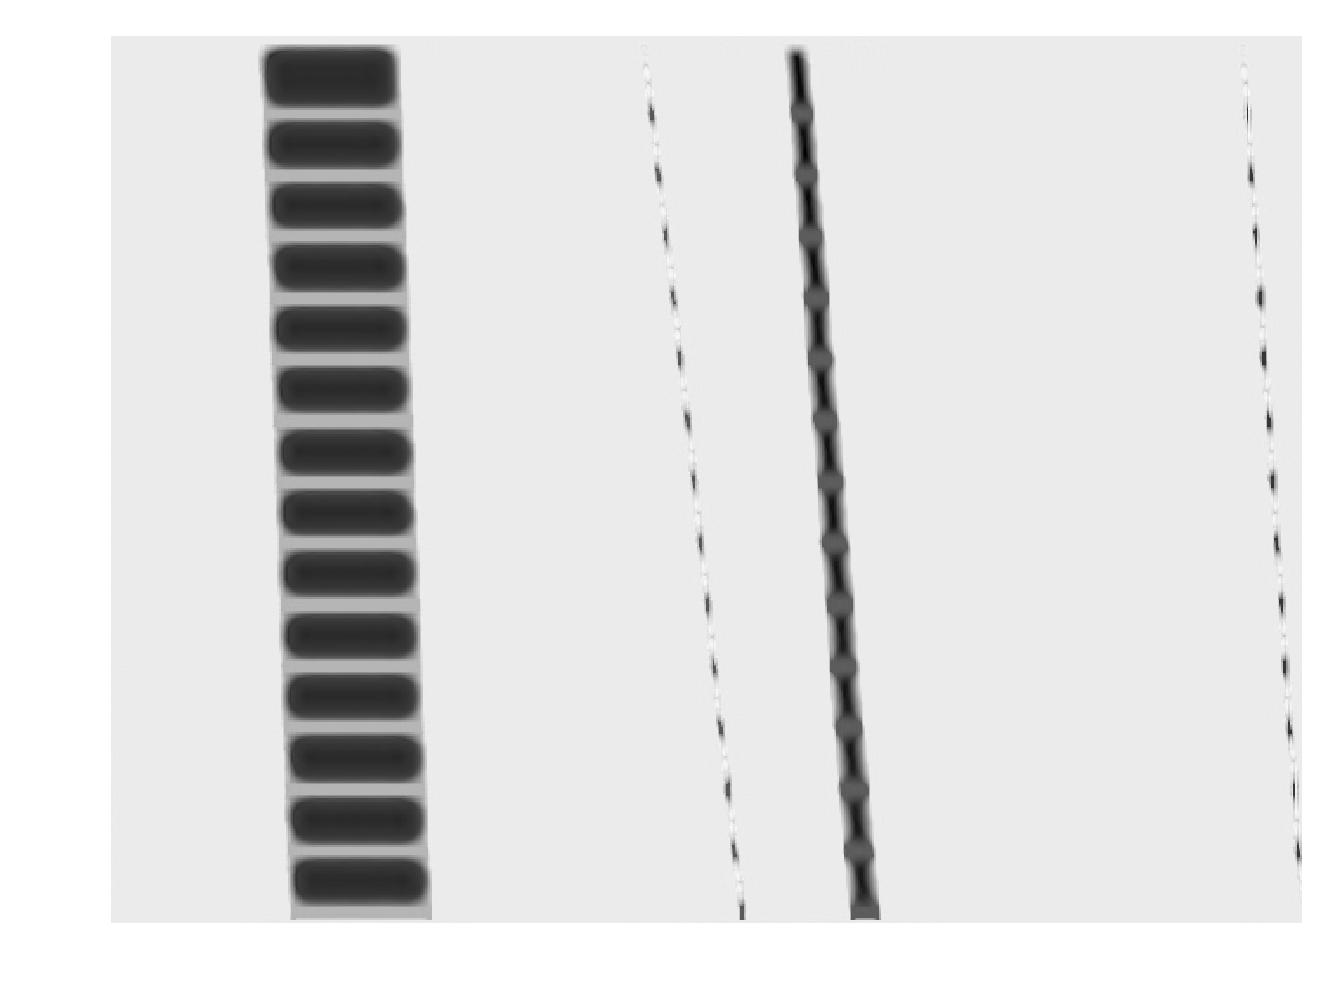
\includegraphics[width = 0.7 \textwidth]{./Diagrams/results/Inpainted/424_8_102_7_10_4_inpainted.png}
\caption{Inpainted EPI corresponding to the strip on Figure~\ref{fig:strip2}}
\label{fig:inpainted2}
\end{figure}

\begin{figure}[h!]
\centering
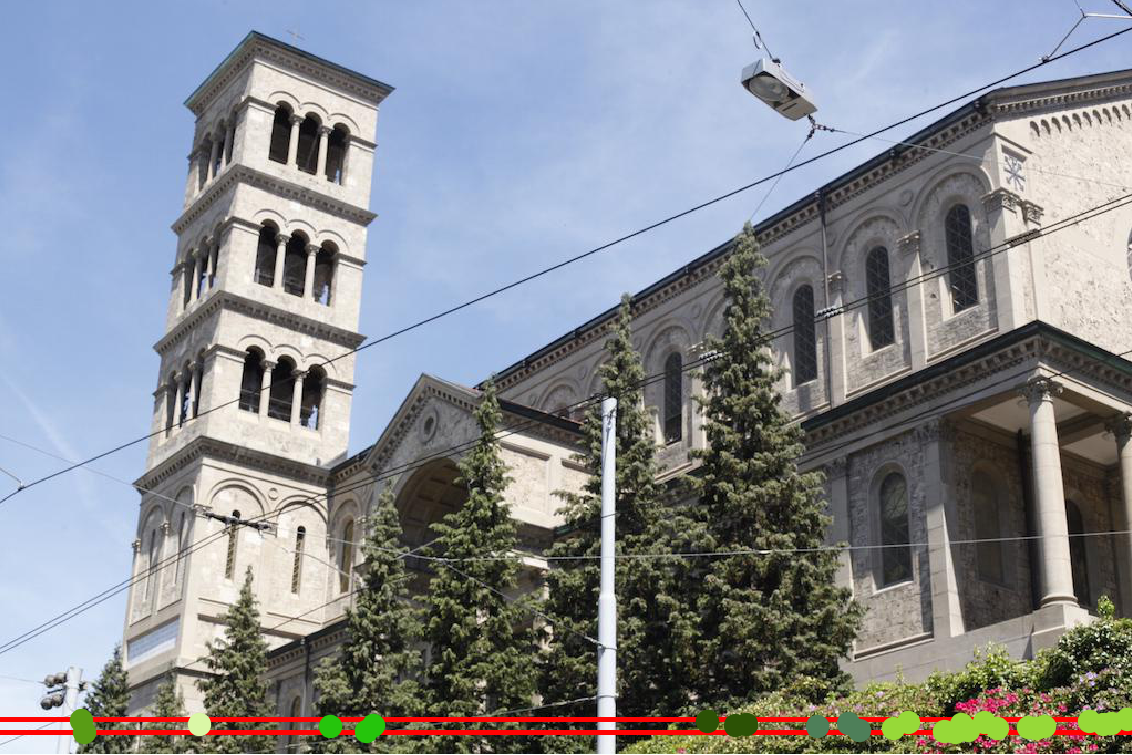
\includegraphics[width = 0.7 \textwidth]{./Diagrams/results/EPIs/306_8_102_7_27_6_strip.png}
\caption{Strip with tracked points}
\label{fig:strip3}
\end{figure}

\begin{figure}[h!]
\centering
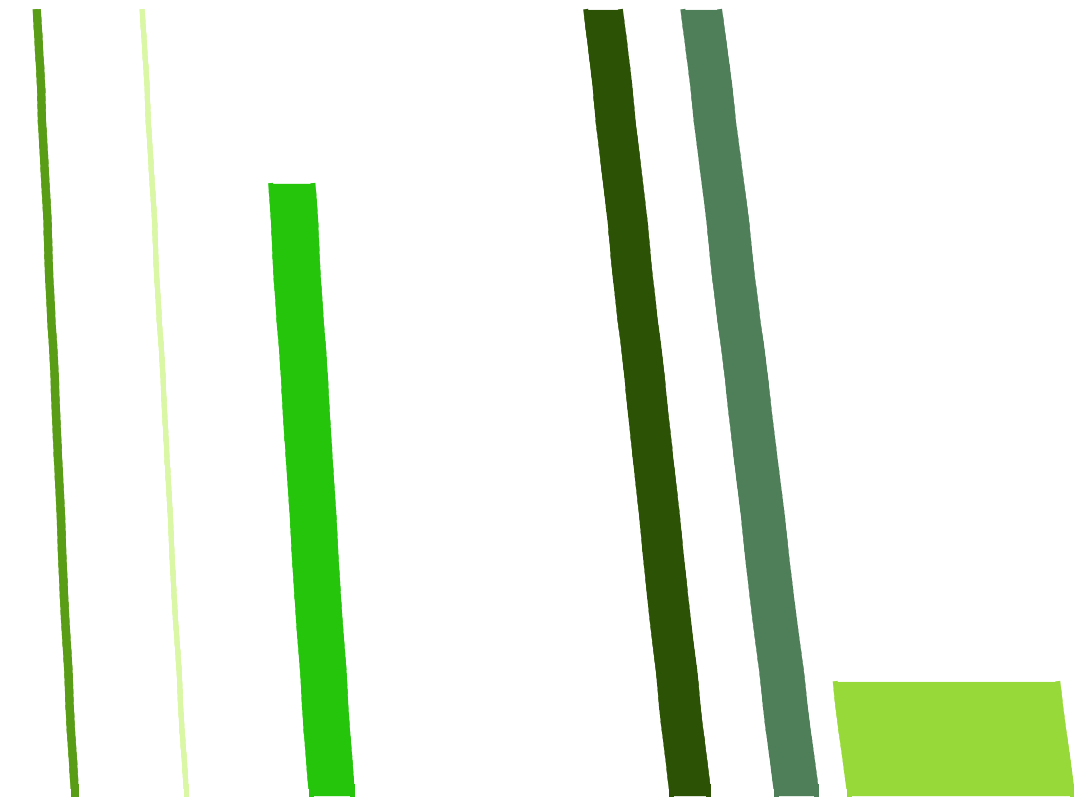
\includegraphics[width = 0.7 \textwidth]{./Diagrams/results/EPIs/306_8_102_7_27_6_dense.png}
\caption{Dense EPI corresponding to the strip on Figure~\ref{fig:strip3}}
\label{fig:dense3}
\end{figure}

\begin{figure}[h!]
\centering
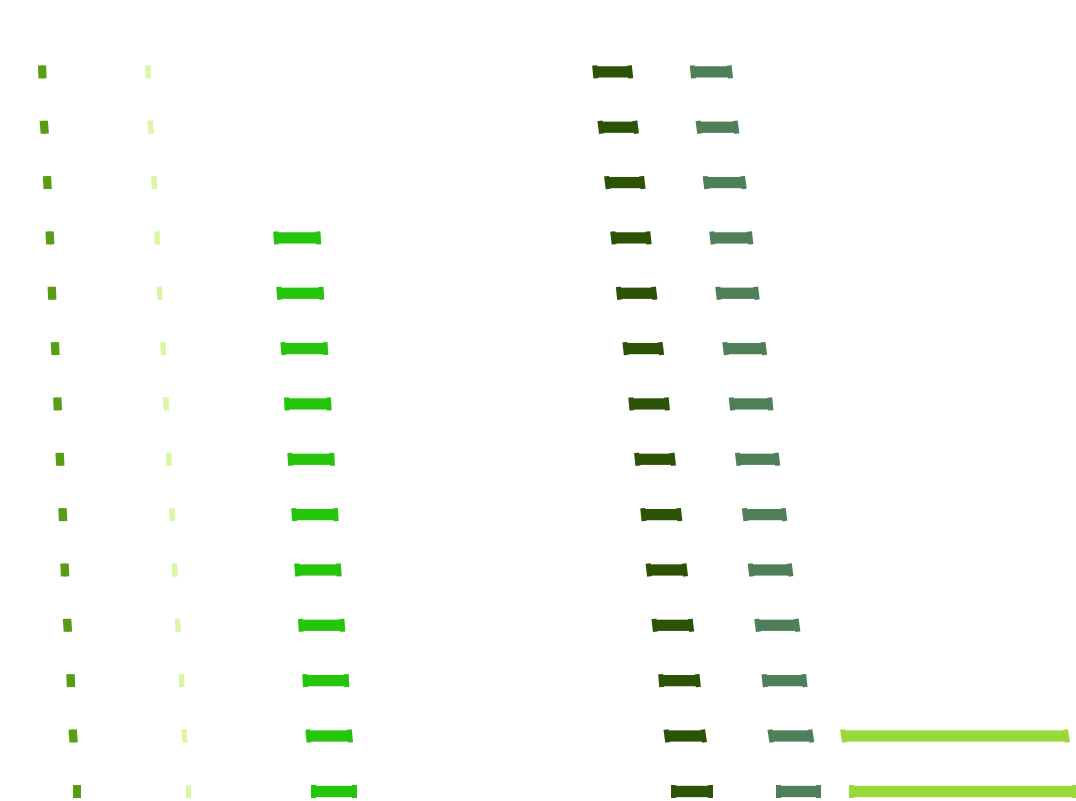
\includegraphics[width = 0.7 \textwidth]{./Diagrams/results/EPIs/306_8_102_7_27_6_sparse.png}
\caption{Sparse EPI corresponding to the strip on Figure~\ref{fig:strip3}}
\label{fig:sparse3}
\end{figure}

\begin{figure}[h!]
\centering
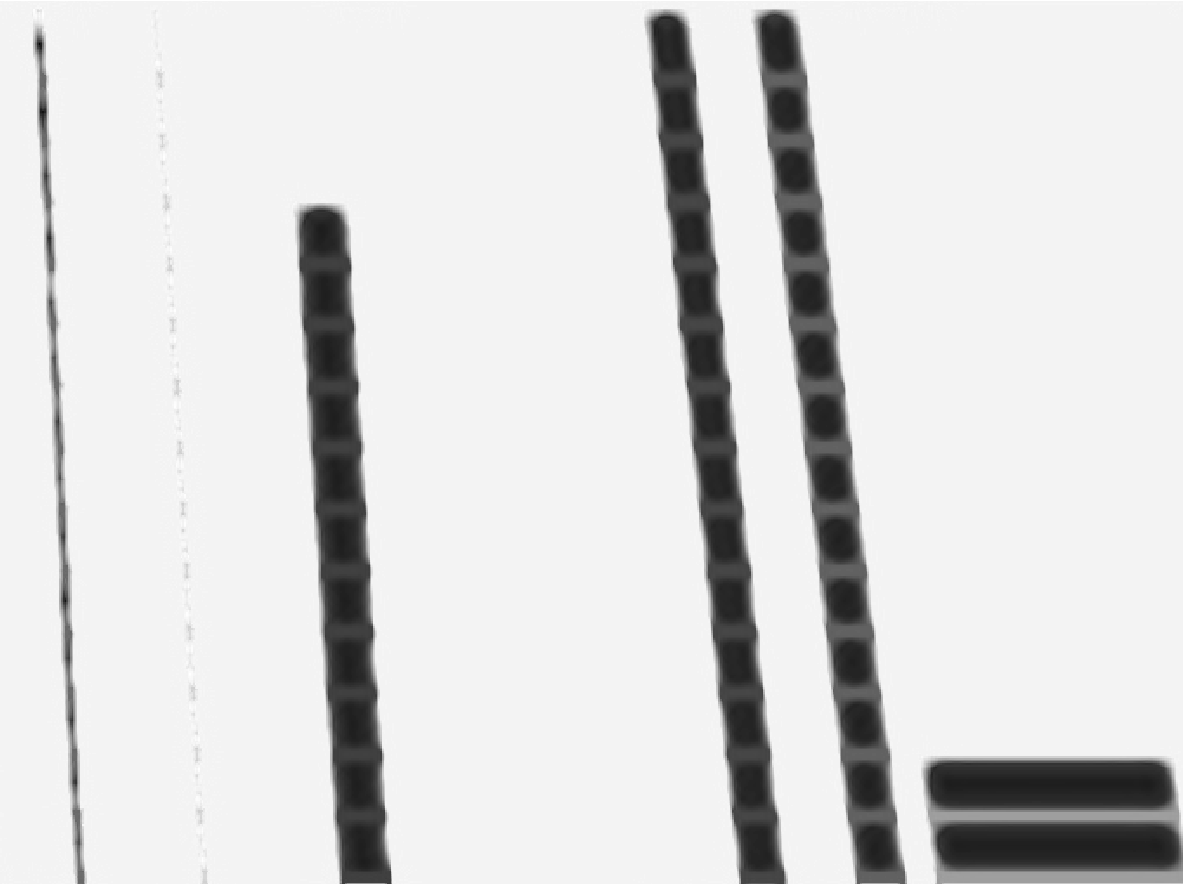
\includegraphics[width = 0.7 \textwidth]{./Diagrams/results/Inpainted/306_8_102_7_27_6_inpainted.png}
\caption{Inpainted EPI corresponding to the strip on Figure~\ref{fig:strip3}}
\label{fig:inpainted3}
\end{figure}

\begin{figure}[h!]
\centering
\includegraphics[width = 0.7 \textwidth]{./Diagrams/results/EPIs/292_8_102_7_34_8_strip.png}
\caption{Strip with tracked points}
\label{fig:strip4}
\end{figure}

\begin{figure}[h!]
\centering
\includegraphics[width = 0.7 \textwidth]{./Diagrams/results/EPIs/292_8_102_7_34_8_dense.png}
\caption{Dense EPI corresponding to the strip on Figure~\ref{fig:strip4}}
\label{fig:dense4}
\end{figure}

\begin{figure}[h!]
\centering
\includegraphics[width = 0.7 \textwidth]{./Diagrams/results/EPIs/292_8_102_7_34_8_sparse.png}
\caption{Sparse EPI corresponding to the strip on Figure~\ref{fig:strip4}}
\label{fig:sparse4}
\end{figure}

\begin{figure}[h!]
\centering
\includegraphics[width = 0.7 \textwidth]{./Diagrams/results/Inpainted/292_8_102_7_34_8_inpainted.png}
\caption{Inpainted EPI corresponding to the strip on Figure~\ref{fig:strip4}}
\label{fig:inpainted4}
\end{figure}


\begin{figure}[h!]
\centering
\includegraphics[width = 0.7 \textwidth]{./Diagrams/results/EPIs/673_10_102_4_48_8_strip.png}
\caption{Strip with tracked points}
\label{fig:strip5}
\end{figure}

\begin{figure}[h!]
\centering
\includegraphics[width = 0.7 \textwidth]{./Diagrams/results/EPIs/673_10_102_7_48_8_dense.png}
\caption{Dense EPI corresponding to the strip on Figure~\ref{fig:strip5}}
\label{fig:dense5}
\end{figure}

\begin{figure}[h!]
\centering
\includegraphics[width = 0.7 \textwidth]{./Diagrams/results/EPIs/673_10_102_7_48_8_sparse.png}
\caption{Sparse EPI corresponding to the strip on Figure~\ref{fig:strip5}}
\label{fig:sparse5}
\end{figure}

\begin{figure}[h!]
\centering
\includegraphics[width = 0.7 \textwidth]{./Diagrams/results/Inpainted/673_10_102_7_48_8_inpainted.png}
\caption{Inpainted EPI corresponding to the strip on Figure~\ref{fig:strip5}}
\label{fig:inpainted5}
\end{figure}

\item \textbf{Fourth step (line detection and depth map computation)}: We used Hough Line Transform on the inpainted EPIs to detect the lines and compute the depth map based on the slopes of the lines; this step will be explained in detail in the Section~\ref{sec:line_detect}.

\end{itemize}

\section{Line detection in inpainted EPIs and depth map computation}
\label{sec:line_detect}

Once we have the inpaited EPIs for our sparse set of views with disparity $d_{max}=7$ pixels, we need to be able to compute the slopes of the lines corresponding to different feature points, and then obtain the depth map; where the depth of a point corresponding to some line in an EPI will be given by Equation~\ref{eq:C1S4E2} in the form of

\begin{equation}
\label{eq:slope_epi}
D = h\frac{\Delta X}{\Delta U}= h\cdot \textrm{slope}
\end{equation}

where $h$ is the focal length of the camera that according to the specifications of the camera used in the data set is $h = 50mm=5\times 10^{-2}m$. In our case, each inpainted picture is imported in the line detection algorithm code as an image of certain $size=[size_x,size_y]$; by specifications of the data set we have that there were 101 taken pictures with a separation of $10$mm from each other with a total time span of $1010mm=1.01m$, the horizontal size in pixels of the used images in the data set is $683px$, therefore to obtain the depth of a point in Equation~\ref{eq:slope_epi} in an unified way and be able to compare the obtained depths in different strips we will need to modify the equation with a normalization term multiplying $m$, obtaining the equation:

\begin{equation}
\label{eq:slope_epi_unified}
D = (0.01m)\cdot \textrm{slope}\cdot\left(\frac{\textrm{size}_x}{\textrm{size}_y}\right)\cdot\left(\frac{1.01m}{683px}\right)
\end{equation}

\bigskip

The resulting depth given by Equation~\ref{eq:slope_epi_unified} has units of $\frac{m^2}{px}$, the transformation from pixels to meters is not straight forward since we would need to know the transformation betweeen the spatial and image coordinates, and for that one should know a priori the actual depth of some fixed point and the correspondance in meters of the pixels of features at that depth; therefore the obtained depth is relative, but that is enough to construct the depth map.

\bigskip

Now that we know how to get the depth of points by its slope in the corresponding epipolar plane image we need to have a way to actually measure the slope of lines on the inpainted epipolar planes images and therefore we need a method to detect lines in an image. There are different methods to detect lines in images, commonly known as edge detectors; one can give as examples the Canny edge detector, the Phase Stretch Transform (PST), the Sobel method and the Hough Line Transform (see \cite{LearnOpenCV}, \cite{MultipleView}, \cite{hough-duda}, \cite{hough-invented} for a detailed explanation of each of this methods). By its easy and fast implementation and its effectiveness we used the Hough line transform to detect lines on the inpainted EPIs. 

\bigskip

The Hough line transform was invented by Richard Duda and Peter Hart in 1972 on their paper "Use of the Hough Transformation to Detect Lines and Curves in Pictures"\cite{hough-duda} and it is actually a generalization of a 1962 patent of Pual Hough\cite{hough-original} who proposed it for analysis of Bubble Chamber photographs for particle detection.

\bigskip

Even it seems as a trivial task for human vision, in automated analysis of digital images, a problem that often arises is the problem of detecting simple shapes as straight lines or circles. Generally an edge detector can be used as a pre-processing stage to obtain image points or image pixels that form part of the analysed curve in the image space. However imperfections in the image data or the edge detector may miss points or pixels on the desired cuves as well as spatial deviations between the ideal theoretical line/circle and the noisy edge points as they are obtained from the edge detector; therefore it is non-trivial to group the extracted edge features to an appropriate set of lines or circles. The Hough transform has as purpose to address this problem by making it possible to perform groupings of edge points into object candidates by performing an explicit voting procedure over a set of parameterized image objects; in this thesis we will just make use of the simplest case of Hough transform that is detecting straight lines and it will be explained in the following.

\bigskip

A line in the image space can be expressed with two variables; for example by the parameters $(m,b)$ in Cartesian coordinates system where $m$ is the slope of the line and $b$ is the $y$-intercept of the line or in Polar coordinates system with parameters $(r,\theta)$ where $r$ is the distance to the origin and $\theta$ the angle with the $x$-axis. For Hough Transforms, we will express lines in the Polar system where a line equation can be written as:

\begin{equation}
\label{eq:polar-lines}
y = \left(-\frac{\cos\theta}{\sin\theta}\right)x+\left(\frac{r}{\sin\theta}\right)
\end{equation} 

this obtained by the relation $r=x\cos\theta+y\sin\theta$.

\bigskip

Given an arbitrary fixed point $(x_0,y_0)\in\mathbb{R}^2$, one can define a family of lines that goes through the points by

\begin{equation}
\label{eq:family-lines}
r_{\theta}=x_0\cos\theta+y_0\sin\theta
\end{equation}

Therefore each pair $(r_{\theta},\theta)$ represents each line that passes by $(x_0,y_0)$.

\bigskip 

By the form of the Equation~\ref{eq:family-lines}, for a given fixed point $(x_0,y_0)$ the plot of the family of lines that goes through it on the domain $\theta$ \textbf{vs.} $r_{\theta}$ is a sinusoid, we will consider only points such that $r>0$ and $0<\theta<2\pi$(see Figure~\ref{fig:family-lines-hough}).

\begin{figure}[h!]
\centering
\includegraphics[width = 0.8 \textwidth]{./Diagrams/family-lines-hough.jpg}
\caption{Plot of $\theta\textrm{vs.}r_{\theta}$ for $x_0=8$ and $y_0=6$}
\label{fig:family-lines-hough}
\end{figure}

\bigskip

We can plot the sinusoidal curves of all the points in an image. If the curves of two different points intersect in the plane $\theta-r_{\theta}$, it means that both points belong to a same line; see the example in Figure~\ref{fig:intersection-hough}.

\begin{figure}[h!]
\centering
\includegraphics[width = 0.8 \textwidth]{./Diagrams/family-lines-hough.jpg}
\caption{Plot of $\theta\textrm{vs.}r_{\theta}$ corresponding to the points $(x_0,y_0)=(8,6)$, $(x_1,y_1)=(4,9)$ and $(x_2,y_2)=(12,3)$}
\label{fig:intersection-hough}
\end{figure}

\bigskip

The three plots in Figure~\ref{fig:intersection-hough} intersect in one single point $(0.925,9.6)$, these coordinates are the parameters $(\theta,r)$ or the line in which $(x_0,y_0)$, $(x_1,y_1)$ and $(x_2,y_2)$ lay; therefore in general, a line can be \textbf{detected} by finding the number of intersections between curves. The more curves intersecting means that the line represented by that intersection have more points. In general we can define a threshold of the minimum number of intersections needed to detect a line. This is what the Hough Line Transform does. It keeps track of the intersection between curves of every point in the image. If the number of intersections is above some threshold, then it declares it as a line with the parameters $(\theta,r_{\theta})$ of the intersection point.

\bigskip 

There are different existing implementations of the Hough line, in Python, C++ and Matlab; in this thesis we used the python implementation using the OpenCV API, cause is very simple to use and fast to run; we made use of the Canny edge detector that is similar to the already explained Shi-Tomasi and for more detail one should check \cite{LearnOpenCV} and the Hough Line Transfom. In order to compute the depth map, we made use of the inpainted EPIs corresponding to strips at different fixed $y$'s; the points were divided by the different features were they belong, those features are enumerated in the following list and pictured in Figure~\ref{fig:feature_points}

\begin{enumerate}
\item Bush 1.
\item Bush 2.
\item Bush 3. 
\item Tree 1.
\item Tree 2.
\item Tree 3.
\item Tree 4.
\item Tree 5.
\item Tree 6.
\item Lamp Post 1.
\item Lamp Post 2.
\item Front Wall.
\item Window 1.
\item Window 2. 
\item Window 3. 
\item Window 4.
\item Pillar 1.  
\item Pillar 2. 
\item Cable 1.
\item Cable 2.
\item Cable 3.
\item High Lamp.
\item Tower.
\end{enumerate} 

\begin{figure}[h!]
\centering
\includegraphics[width = 0.9 \textwidth]{./Diagrams/results/data_set/feature_points.png}
\caption{Features of the Church with tracked points}
\label{fig:feature_points}
\end{figure}

Once we have points associated to features, we compute the depth of this points at different fixed $y$-strips finding out that for a fixed $y$-strip the points of a certain feature have relatively the same depth, therefore we assigned a depth to a feature for a fixed $y$. As we already mentioned we used the OpenCV python API as well as some python code for computing the depth map with this method, the code can be found in Appendix~\ref{sec:Appendix_D} and the obtained results are in the tables~\ref{table1} to~\ref{table6} where the values at each height $y$ (where the different strips are centered at) are the obtained depth of the points of that feature at that height in meters$^2$/pixels and whenever occur a blank space means that such feature has not points in such height (is worth to mention that the heights are measured from bottom to top, i.e.\ the bigger the height, the lower in the picture); this values describe completly the depth map, if one would like to visualize them in a refocusing-type application we should perform the so called light field rendering, where one finds contours of the corresponding features and apply a gaussian filter to defocused the elements that are not at the same depth, but this is not part of this thesis and will be taken as a future development goal. One can use as a guide of the heights Figure~\ref{fig:feature_points_grid}. 

\begin{figure}[h!]
\centering
\includegraphics[width = 0.9 \textwidth]{./Diagrams/results/data_set/feature_points_grid.png}
\caption{Features of the Church with tracked points with grid of heights}
\label{fig:feature_points_grid}
\end{figure}


\begin{table}[!htb]
\centering
    \begin{tabular}{| c | c | c | c | c | c | c | c | c |}
    \hline
    feature/height(px) & 680 & 673 & 664 & 632 & 616 & 600 & 584 & 568 \\ \hline
		 Bush1 & 0.0161 & 0.0157 & 0.0158 & 0.0156 & 0.0157 & 0.0161 & 0.0160 & 0.0158\\ \hline
		 Bush2 & 0.0217 & 0.0221 & 0.0221 & 0.0220 &  &  &  & \\ \hline	
		 Bush3 & 0.0257 & 0.0261 & 0.0260 & 0.0258 & 0.0258 &  &  & \\ \hline	
		 Tree1 & 0.0284 & 0.0285 & 0.0286 & 0.0285 & 0.0285 & 0.0286 & 0.0287 & 0.0291 \\ \hline	
		 Tree2 &  &  & 0.0442  &  &  & 0.045  & 0.046 & 0.045 \\ \hline	
		 Tree3 & 0.0501 & 0.0502 & 0.0501 & 0.0499 & 0.0498 & 0.0502 & 0.0500 & 0.0501\\ \hline	
		 Tree4 & 0.0594 & 0.0591 & 0.0590 & 0.0589 & 0.0590 & 0.0593 & 0.0595 & 0.0594\\ \hline	
		 Tree5 & 0.0801 & 0.0799 & 0.0798 & 0.0800 & 0.0801 & 0.0798 & 0.0799 & 0.0800\\ \hline	
		 Tree6 & 0.1001 & 0.0998 & 0.0999 & 0.0998 & 0.1003 & 0.1002 &  & \\ \hline	
     LampPost1 &  &  & & 0.0181 &  & 0.0180 & 0.0182 &  \\ \hline
		 LampPost2 &  &  &  & 0.1123 & 0.1122  &  &  & \\ \hline
		 FrontWall &  &  &  &  &  &  &  & \\ \hline
		 Window1 &  &  &  &  &  &  &  & \\ \hline
		 Window2 &  &  &  &  &  &  &  & \\ \hline
		 Window3 &  &  &  &  &  &  &  & \\ \hline
		 Window4 &  &  &  &  &  &  &  & \\ \hline
		 Pillar1 &  &  &  &  &  &  &  & \\ \hline
		 Pillar2 &  &  &  &  &  &  &  & \\ \hline
		 Cable1 &  &  &  &  &  &  &  & \\ \hline
	   Cable2 &  &  &  &  &  &  &  & \\ \hline
	   Cable3 &  &  &  &  &  &  &  & \\ \hline
		 HighLamp &  &  &  &  &  &  &  & \\ \hline
	   Tower &  &  &  &  &  &  &  & \\ \hline
    \end{tabular}
		\caption{Depth of features in $m^2/px$ at different heights in $px$}\label{table1}
\end{table}

\begin{table}[!htb]
\centering
    \begin{tabular}{| c | c | c | c | c | c | c | c | c |}
    \hline
    feature/height(px) & 552 & 536 & 520 & 504 & 488 & 472 & 456 & 440\\ \hline
		 Bush1 & 0.0157 &  &  &  &  &  &  & \\ \hline
		 Bush2 &  &  &  &  &  &  &  & \\ \hline	
		 Bush3 &  &  &  &  &  &  &  & \\ \hline	
		 Tree1 & 0.0291 & 0.0292 & 0.0290 & 0.0291 &  &  &  & 0.030 \\ \hline	
		 Tree2 & 0.0461 & 0.0456 & 0.0460 & 0.0459 &  &  & 0.0461 & 0.0461\\ \hline	
		 Tree3 & 0.0495 & 0.0496 &  & 0.0497 & 0.0498 & 0.0499 & 0.0495 & 0.0501 \\ \hline	
		 Tree4 & 0.0594 &  &  &  &  &  &  & \\ \hline	
		 Tree5 &  &  &  &  &  &  &  & \\ \hline	
		 Tree6 &  &  &  &  &  &  &  & \\ \hline	
     LampPost1 & 0.0181 & 0.0180 & 0.0182 & 0.0183 &  & 0.0182 & 0.0179 & 0.0180 \\ \hline
		 LampPost2 &  &  &  &  &  &  &  & \\ \hline
		 FrontWall &  &  &  &  &  &  &  & \\ \hline
		 Window1 &  &  &  &  &  &  &  & \\ \hline
		 Window2 &  &  &  &  &  &  &  & \\ \hline
		 Window3 &  &  &  &  &  &  &  & \\ \hline
		 Window4 &  & 0.0391 &  &  &  &  &  & \\ \hline
		 Pillar1 &  &  &  &  &  &  &  & 0.0054 \\ \hline
		 Pillar2 &  & 0.0251 &  &  &  &  &  & \\ \hline
		 Cable1 &  &  &  &  & 0.0020 &  &  & \\ \hline
	   Cable2 &  &  &  &  &  & 0.0701 & 0.0608 & \\ \hline
	   Cable3 &  &  &  &  &  &  &  & \\ \hline
		 HighLamp &  &  &  &  &  &  &  & \\ \hline
	   Tower &  &  &  &  &  &  &  & \\ \hline
    \end{tabular}
		\caption{Depth of features in $m^2/px$ at different heights in $px$}\label{table2}
\end{table}

\begin{table}[!htb]
\centering
    \begin{tabular}{| c | c | c | c | c | c | c | c | c |}
    \hline
    feature/height(px) & 424 & 408 & 392 & 376 & 360 & 344 & 328 & 322\\ \hline
		 Bush1 &   &   &  &  &  &  &  & \\ \hline
		 Bush2 &  &  &  &  &  &  &  & \\ \hline	
		 Bush3 &  &  &  &  &  &  &  & \\ \hline	
		 Tree1 &  &  & 0.0332 & 0.0341 & 0.0341 &  & 0.0335 & \\ \hline	
		 Tree2 &  & 0.0459 &  &  &  &  &  & \\ \hline	
		 Tree3 & 0.0502 & 0.0500 & 0.0501 &  & 0.0502 & 0.0499 &  & \\ \hline	
		 Tree4 &  &  &  &  &  &  &  & \\ \hline	
		 Tree5 &  &  &  &  &  &  &  & \\ \hline	
		 Tree6 &  &  &  &  &  &  &  & \\ \hline	
     LampPost1 &  &  &  &  & 0.0180 & 0.0181 &  & \\ \hline
		 LampPost2 &  &  &  &  &  &  &  & \\ \hline
		 FrontWall &  &  &  &  &  &  &  & \\ \hline
		 Window1 &  &  &  &  &  &  &  & 0.0601\\ \hline
		 Window2 &  &  &  &  &  &  &  & \\ \hline
		 Window3 &  & 0.0522 &  &  &  &  &  & \\ \hline
		 Window4 &  &  &  &  &  &  &  & \\ \hline
		 Pillar1 &  &  &  &  &  &  &  & \\ \hline
		 Pillar2 &  &  &  &  &  & 0.0256 &  & \\ \hline
		 Cable1 &  &  &  &  &  &  & & \\ \hline
	   Cable2 &  &  &  &  &  &  & 0.0212 & \\ \hline
	   Cable3 &  &  &  &  &  &  &  & \\ \hline
		 HighLamp &  &  &  &  &  &  &  & \\ \hline
	   Tower & 0.0995 &  & 0.1002  & 0.1003  & 0.1002 & 0.1001 & 0.1002 & 0.0996 \\ \hline
    \end{tabular}
		\caption{Depth of features in $m^2/px$ at different heights in $px$}\label{table3}
\end{table}

\begin{table}[!htb]
\centering
    \begin{tabular}{| c | c | c | c | c | c | c | c | c |}
    \hline
    feature/height(px) & 312 & 306 & 300 & 292 & 280 & 264 & 248 & 232 \\ \hline
		 Bush1 &  &  &  &  &  &  &  & \\ \hline
		 Bush2 &  &  &  &  &  &  &  & \\ \hline	
		 Bush3 &  &  &  &  &  &  &  & \\ \hline	
		 Tree1 &  &  &  &  &  &  &  & \\ \hline	
		 Tree2 &  &  &  &  &  &  &  & \\ \hline	
		 Tree3 &  &  &  &  &  &  &  & \\ \hline	
		 Tree4 &  &  &  &  &  &  &  & \\ \hline	
		 Tree5 &  &  &  &  &  &  &  & \\ \hline	
		 Tree6 &  &  &  &  &  &  &  & \\ \hline	
     LampPost1 &  &  &  &  &  &  &  & \\ \hline
		 LampPost2 &  &  &  &  &  &  &  & \\ \hline
		 FrontWall &  &  &  &  &  &  &  & 0.0051\\ \hline
		 Window1 &  &  &  &  &  &  &  & \\ \hline
		 Window2 &  &  &  &  & 0.0402 &  &  & \\ \hline
		 Window3 &  &  &  &  &  &  &  & \\ \hline
		 Window4 &  &  &  &  &  &  &  & \\ \hline
		 Pillar1 &  &  &  &  &  &  &  & \\ \hline
		 Pillar2 &  &  &  &  &  &  &  & \\ \hline
		 Cable1 &  &  &  &  &  &  &  & \\ \hline
	   Cable2 &  &  &  &  & 0.0131 &  &  & \\ \hline
	   Cable3 &  &  &  &  &  &  &  & \\ \hline
		 HighLamp &  &  &  &  &  &  &  & \\ \hline
	   Tower &  &  &  &  &  & 0.1001 & 0.0999 & 0.1003 \\ \hline
    \end{tabular}
		\caption{Depth of features in $m^2/px$ at different heights in $px$}\label{table4}
\end{table}

\begin{table}[!htb]
\centering
    \begin{tabular}{| c | c | c | c | c | c | c | c | c |}
    \hline
    feature/height(px) & 216 & 200 & 168 & 152 & 136 & 120 & 104 & 88\\ \hline
		 Bush1 &  &  &  &  &  &  &  & \\ \hline
		 Bush2 &  &  &  &  &  &  &  & \\ \hline	
		 Bush3 &  &  &  &  &  &  &  & \\ \hline	
		 Tree1 &  &  &  &  &  &  &  & \\ \hline	
		 Tree2 &  &  &  &  &  &  &  & \\ \hline	
		 Tree3 &  &  &  &  &  &  &  & \\ \hline	
		 Tree4 &  &  &  &  &  &  &  & \\ \hline	
		 Tree5 &  &  &  &  &  &  &  & \\ \hline	
		 Tree6 &  &  &  &  &  &  &  & \\ \hline	
     LampPost1 &  &  &  &  &  &  &  & \\ \hline
		 LampPost2 &  &  &  &  &  &  &  & \\ \hline
		 FrontWall &  &  &  &  &  &  &  & \\ \hline
		 Window1 &  &  &  &  &  &  &  & \\ \hline
		 Window2 &  &  &  &  &  &  &  & \\ \hline
		 Window3 &  &  &  &  &  &  &  & \\ \hline
		 Window4 &  &  &  &  &  &  &  & \\ \hline
		 Pillar1 &  &  &  &  &  &  &  & \\ \hline
		 Pillar2 &  &  &  &  &  &  &  & \\ \hline
		 Cable1 &  &  &  &  &  &  &  & \\ \hline
	   Cable2 &  & 0.0015 &  &  &  &  &  & \\ \hline
	   Cable3 &  &  &  &  &  &  &  & \\ \hline
		 HighLamp &  &  &  &  &  & 0.0009 &  & \\ \hline
	   Tower & 0.1002 & 0.0998 &  & 0.0999 & 0.1002 & 0.0998 & 0.1001 & \\ \hline
    \end{tabular}
		\caption{Depth of features in $m^2/px$ at different heights in $px$}\label{table5}
\end{table}

\begin{table}[!htb]
\centering
    \begin{tabular}{| c | c | c | c | c | c | c | c | c |}
    \hline
    feature/height(px) & 72 & 56\\ \hline
		 Bush1 &  &  \\ \hline
		 Bush2 &  &  \\ \hline	
		 Bush3 &  &  \\ \hline	
		 Tree1 &  &  \\ \hline	
		 Tree2 &  &   \\ \hline	
		 Tree3 &  &   \\ \hline	
		 Tree4 &  &   \\ \hline	
		 Tree5 &  &   \\ \hline	
		 Tree6 &  &    \\ \hline	
     LampPost1 &  &  \\ \hline
		 LampPost2 &  &  \\ \hline
		 FrontWall &  &  \\ \hline
		 Window1 &  &  \\ \hline
		 Window2 &  &  \\ \hline
		 Window3 &  &  \\ \hline
		 Window4 &  &  \\ \hline
		 Pillar1 &  &   \\ \hline
		 Pillar2 &  &  \\ \hline
		 Cable1 &  &  \\ \hline
	   Cable2 &  &  \\ \hline
	   Cable3 &  & 0.0020\\ \hline
		 HighLamp & 0.0008 & 0.0007  \\ \hline
	   Tower &  & \\ \hline
    \end{tabular}
		\caption{Depth of features in $m^2/px$ at different heights in $px$}\label{table6}
\end{table}

It could also be interesting to have depth map not by feature but by $x$ position, therefore one could make a heat map with the depth which will give us a more effective way to analyse it; the issue with this approach is that hardly more than the already tracked points can be tracked by the common tracking algorithms; this could be improved in the future using some other transformation like iterative feature extractors like Convolutional Neural Networks\cite{DCNN} to have a better corner detector and to be able to track more points; even though this approach works very well and the comparison with the existent light field recovery methods for approaching the depth map of a scene, in the next section we will shortly review this. 

\section{Performance and results comparison with previews works}
\label{sec:perform_results}

We already mentioned several times the computer system that was used is a low end MacBook whose processor and gpu are by far not the best in the commercial market and are even worse in comparison with the high-end servers used some researcher on the area. 

\bigskip

In the last sections we got the next running times on finishing the whole pipeline of light field reconstruction:

\begin{itemize}
\item \textbf{Point tracking}: 16.36 seconds.
\item \textbf{Sparse EPI painting}: 9.46 seconds (43 EPIs, 0.22 seconds for each).
\item \textbf{Sparse EPI inpainting}: 666.50 (43 inpeinted EPIs, 15.50 seconds for each).
\item \textbf{Line detection and depth map computation}: 0.43 seconds (43 EPIs, 0.01 seconds for each).
\end{itemize}

This gives a total of 692.75 seconds (around 11 seconds) to reconstruct the Light Field and compute the Depth Map. With this estimates we can make a comparison with the performance of the other works on light field reconstruction; to be clear it is important to mention that along the different approaches and works on light field reconstruction the goals of the methods are different although the main purpose is the same. In this particular thesis we wanted to present a method that is easy to implement, free, open source, fast and that doesn't require very sofisticated systems; the limitations of our method comes when one wants to recover high definition light fields on images with few corners (few points to track with Lucas-Kanade), but for our particular dataset works perfectly. Having this in mind one can proceed with the comparison with the other works.

\begin{enumerate}
\item \textit{"Compressive Light Field Photograph using Overcomplete Dictionaries and Optimized Projections"} (by Wetzstein et all, check \cite{CompressedMIT}): Their approach made use of coded mask on an imaging lens to emulate a microlenses array on a SLR Camera (Nikon 105 mm f/2.8D). They learned a dictionary for 3D-light field with a data set of scenes (light field atoms) using an optimization problem as learning algorithm and then using this dictionary they performed compression of high resolution light fields using the LASSO algorithm \cite{LASSO} and the elements of the learned dictionary as representation system. In the implemenation they learned $1.7\times$ overcomplete dictionary consisting of $5,000$ light field atoms with a memory footprint of about 111 MB. 

The employed the privative Sparse Modeling Software \cite{SparseSoft} on a workstation equipped with a 24-core Intel Xeon processor and 200 GB RAM, and it took about 10 hours. Finally the Light Field Sparse Reconstruction was performed in parallel on an 8-core Intel I7 workstation with 16 GB RAM, the reconstructions for three color channels took about 18 hours for each light field, which gave a total of 28 hours of processing for the reconstruction of one light field (almost 152 times slower than our method). Even this method is clearly slower than our approach the main difference is the resolution of the recovered light field almost 4 times higher than ours; though since it is based of a dictionary learned with a limited set of coded light fields, the recovery is very biased. 

\item \textit{"3D Reconstruction and Rendering from High Resolution Light Fields"} (ETH Zurich's PhD Thesis by C. Kim, check \cite{Kim-Disney}): The data set that we used was actually acquired by the Research Group of Changil Kim on the ETH Zurich; the hardware was explained in detail on Section~\ref{sec:Sparse-acquisition}. They used the raw images with a resolution of $4080\times 2720$ pixels, we used a downsampled version of the pictures of $1024\times683$ pixels. The geometric representation used by Kim is the same as we used, Epipolar Plane Images, but in this case densely sampled using a fine-to-coarse depth estimation (starting with parts of highest resolution and moving to less clear parts), this premits them to have a high resolution EPIs and have depth estimation in small neighbourhood of individual pixels. For the Light Field Recovery they used a desktop PC with an Intel Core i7 3.2 GHz and an NVidia GTX 680 graphics card, with a total of 100 views at 21 MP resolution the computation of a very detailed depth map took around 100 minutes (around 10 times slower than our method). 

\item \textit{"Light Field Reconstruction Using Shearlet Transform"} (by S. Vagharshakyan et al., check \cite{LF-Shearlets}): The recovery method and implementation on this thesis is strongly inspired on the work of Vagharshakyan; the biggest difference is that Vagharshakyan et al just explained the theory behind the Light Field reconstruction, but not the actual implementation of the whole pipeline, we cannot perform a proper benchmark of comparison with this work, since they just presented the PSNR (Peak Signal-to-Noise Ratio) as a performance reference; in our case it is not so important to have a high PSNR as long as the lines of the inpainted EPIs are clear enough to be detected with the Hough Line Transform, which actually happened.

As in our case Vagharshakyan et al.\ used publicly available datasets since they did not have the necessary hardware to actually acquire the whole set of views. For the reconstruction algorithm they used two privative software: DERS (Depth Estimation Reference Software) and VSRS (View Synthesis Reference Software), both developed as part of the Free Viewpoint TeleVision (FTV) project of the ISO/IEC Moving Pictures Experts Group MPEG (check \cite{DERS} and \cite{VSRS} for a detailed explanation of this two pieces of software). We have no benchmarks of the reconstruction algorithm performed by VSRS+DERS but we know that Vagharshakyan et al.\ used as Shearlet System generator the matlab version of Shearlab 3D; in our case we used the julia version of Shearlab written by the autor of this thesis, it was already proven that the julia version is faster than the matlab version (check the benchmarks on \url{https://github.com/arsenal9971/Shearlab.jl/tree/master/benchmarks}), so it is expected that our implementation is faster than the one of Vagharshakyan and his group. 
\end{enumerate}

The last items just showed that the Light Field reconstruction method with the complete pipline presented in this thesis is speed-wise better than other methods proposed in the pass; even though our approach has a different goal than them at the end one would like to perform some features like image refocusing or depth estimation applied in computer vision (in particular autonomous driving) and our method is good enough for this purposes; of course we still can perform a lot of different applications with the estimated depth map, like light field 3D rendering and image refocusing but we will let this for future work; this and other planned future developments will be discussed in the next chapter. 

\chapter{Conclusion and outlook}

Template of Conclusion, \cite{Bolles}


\begin{appendices}
\chapter{Code for point tracking}
\label{sec: Appendix A}

The code used in the python API of OpenCV to detect the N strongest corners and track them through the 101 different views in the Church data set is presented in the following:

\lstinputlisting[language=Python]{./Code_notebooks/detecting_tracking.py}


\chapter{Code for point tracking}
\label{sec:Appendix_A}

The code used in the python API of OpenCV to detect the N strongest corners and track them through the 101 different views in the Church data set is presented in the following:

\lstinputlisting[language=julia]{./Code_notebooks/detecting_tracking.py}


\end{appendices}

%----------------------------------------------------------------------------------------
%	THESIS CONTENT - APPENDICES
%----------------------------------------------------------------------------------------

%\appendix % Cue to tell LaTeX that the following "chapters" are Appendices

% Include the appendices of the thesis as separate files from the Appendices folder
% Uncomment the lines as you write the Appendices

%\include{Appendices/AppendixA}
%\include{Appendices/AppendixB}
%\include{Appendices/AppendixC}

%----------------------------------------------------------------------------------------
%	BIBLIOGRAPHY
%----------------------------------------------------------------------------------------
\begin{thebibliography}{90}

\bibitem{Bolles}
	R.C. Bolles, H.H. Baker, D. H. Marimont,
  \emph{Epipolar-plane image analysis and approach to determining structure from motion},
  International Journal of Computer Vision, 1:7-55,
  1987.

\bibitem{Gitta-alpha}
	G. Kutyniok, M. Genzel,
	\emph{Asymptotic analysis of inpainting via universal shearlet Systems},
	SIAM Journal on Imaging Sciences, 7(4), 2301-2339,
	2014

\bibitem{LF-Shearlets}
	S. Vagharshakyan, R. Bregovic, A. Gotchev,
	\emph{Light field reconstruction using shearlet transform},
	IEEE Transactions on Pattern Analysis and Machine Intelligence, P(99),
	2017

\bibitem{Adelson-Plenoptic}
	E.H. Aderson and J.R. Bergen,
	\emph{The plenoptic function and the elements of early vision},
	Vision and Modeling Group, MIT Media Laboratory, MIT, 1991 

\bibitem{Liang}
	C.-K. Liang, Y.-C- Shih, H.Chen,
	\emph{Light field analysis for modeling image formation},
	IEEE Trans. Image Processing, 20(2), 446-460, 
2011

\bibitem{Kim-Disney}
	C. Kim,
  \emph{3D Reconstruction and Rendering from High Resolution Light Fields},
	Diss. ETH No. 22933, 
	2015
  
\bibitem{Ives}
	H. Ives, 
	\emph{Parallax Stereogram and Process of Making Same}
	US patent 725, 567
	1903

\bibitem{Lippmann}
	G. Lippmann, 
	\emph{La Photographie Int\'egrale},
	Academie des Sciences 146, 446-451,
  1908

\bibitem{AdelsonBergen}
	E.H. Adelson, J. R. Bergen,
	\emph{The plenoptic function and the elemnts of early vision},
	Computational Models of Visual Processing, pages 3-20,
	1991

\bibitem{Tomasiearly}
	C. Tomasi,
	\emph{Early Vision},
	Encyclopedia of Cognitive Science, Level 2, 
   2006

\bibitem{CompressedMIT}
	K. Marwah, G. Wetzstein, Y. Bando, R. Raskar,
	\emph{Compressive Light Field Photography using Overcomplete Dictionaries and Optimized Projections},
	ACM Transactions on Graphics (SIGGRAPH), 32(4), 
	2013

\bibitem{Raytrix}
	C. Perwass, L. Wietzke,
	\emph{Single lens 3D-camera with extended depth-of-field},
	Human Vision and EleBuckheit and Donoho (1995)maging 2012, 829108,
	2012

\bibitem{Lytro}
	R. Ng, M. Levoy, M. Br\'edif, G. Duval, M. Horowitz, P. Hanrahan,
	\emph{Light field photography with a hand-held plenoptic camera},
	Technical Report CSTR 2005-2, Stanford University, 
	2005

\bibitem{AdelsonWang}
	E.H. adelson, J. Y. A. Wang,
	\emph{Single lens stereo with a plenoptic camera},
	IEEE International Conference on Computer Vision, 
	2007

\bibitem{Joshi}
	N. Joshi, W. Matusik, S. Avidan,
	\emph{Natural video matting using camera arrays},
	ACM Transactions on Graphics, 25(3), 779-786,
	2006

\bibitem{Veeraraghavan}
	A. Veeraraghavan, R. Raskar, A. K. Agrawal, A. Mohan and J. Trumblin, 
	\emph{Dappled photography: Mask enhanced cameras for heterodyned light fields and coded aperture refocusing},
	ACM Transactions on Graphics, 26(3), 1-69,
	2007

\bibitem{Wetzstein}
	G. Wetzstein, I. Ihrke, W. Heidrich,
	\emph{On plenoptic multiplexing and reconstruction},
	International Journal of Computer Vision, 101(2), 384-400,
	2013

\bibitem{Levoy}
	M. Levoy, P. Hanrahan,
	\emph{Light field rendering},
	Proceedings of ACM SIGGRAPH, 31-42,
	1996

\bibitem{Gortler}
	S. J. Gortler, R. Grzeszczuk, R. Szeliski, M. F. Cohen, 
	\emph{The Lumigraph},
	Proceedings of ACM SIGGRAPH, 43-54,
	1996

\bibitem{Kim-Zimmer}
	C. Kim, H. Zimmer, Y. Pritch, A. Sorkine-Hornung, M. Gross,
	\emph{Scene reconstruction from high spatio-angular resolution light fields},
	ACM Trans. Grpah, 32(4), 73:1-73:2, 
	2013 

\bibitem{Isaksen}
	A. Isaksen, L. McMillan, S.J. Gortler, 
	\emph{Dynamically Reparameterized Light Fields},
	ACM SIGGRAPH, ACM Press, 297-306,
	2000

\bibitem{Javidi}
	B. Javidi, F. Okano, 
	\emph{Three-Dimensional Television, Video and Display Technologies},
	Springer-Verlag,
	2012

\bibitem{Ng-micro}
	M. Levoy, R. Ng, A. Adams, M. Footer, M. Horowitz,
	\emph{Light Field Microscopy},
	ACM Transactions on Graphics, Proceedings of SIGGRAPH, 25(3),
	2006

\bibitem{Pegard}
	N. C. P\'egard, H. Y. Liu, N. Antipa, M. Gerlock, H. Adesnik, L. Waller,
	\emph{Compressive light-field microscopy for 3D neural activity recording},
	Optica 3, 5, 517-524,
	2016

\bibitem{Raskar}
	R. Raskar, A. Agrawal, C. Wilson, A. Veeraraghavan,
	\emph{The Discrete Focal Stack Transform},
	Proc. ACM SIGGRAPH, 56
	2008

\bibitem{Bolles}
	R. C. Bolles, H. H. Baker,
	\emph{Epipolar-Plane Image Analysis: An Approach to Determining Structure from Motion},
	International Journal of Computer Vision, 1, 7-55,
	1987

\bibitem{Gupta}
	R. Gupta, R. I. Hartley, 
	\emph{Linear pushbroom cameras},
	IEEE Transactions on Pattern Analysis and Machine Intelligence, 19(9), 963-975,
	1997

\bibitem{LearnOpenCV}
	G. Bradski, A. Kaehler,
	\emph{Learning OpenCV},
	O'Reilly Media, 2008

\bibitem{MultipleView}
	R. Hartley, A Zisserman,
	\emph{Multiple view geometry in computer vision},
	Cambridge University Press,
	2004

\bibitem{ChangilPhD}
	C. Kim, 
	\emph{3D Reconstruction and Rendering from High Resolution Light Fields},
	PhD Thesis of ETH Zurich, 2015

\bibitem{PointCloud}
	K. Wolff, C. Kim, H. Zimmer, C. Schroers, M. Botsch, O. Sorkine-Hornung, A. Sorkine-Hornung,
	\emph{Point Cloud Noise and Outlier Removal for Image-Based 3D Reconstruction},
	3D International Conference on 3D Vision (3DV), 2016

\bibitem{SceneRec}
	C. Kim, H. Zimmer, Y. Pritch, A. Sorkine-Hornung, M. Gross,
	\emph{Scene Reconstruction from High Spatio-Angular Resolution Light Fields},
	ACM SIGGRAPH, 2013

\bibitem{StructMot}
	T. Basha, S. Avidan, A. Sorkine-Hornung, W. Matusik,
	\emph{Structure and Motion from Scene Registration},
	IEEE Conference on Computer Vision Pattern Recognition (CPVR) 2012
	
\bibitem{SIFT}
	D. G. Lowe,
	\emph{Distinctive Image Features from Scale-Invariant Keypoints},
	International Journal of Computer Vision, 60, 91,
	2004 

\bibitem{MVision}
	D. Vernon,
	\emph{Machine Vision},
	Prentice-Hall, p. 98-99, 214,
	1991
	
\bibitem{HarrisCorner}
	C. Harris, M. Stephens, 
	\emph{A combined corner and edge detector},
	In Proc.\ of Foruth Alvey Vision Conference, 147-151,
	1988

\bibitem{ShiTomasi}
	J. Shi, C. Tomasi,
	\emph{Good Features to Track},
	Vision and Pattern Recognition (CVPR94)i, 593-600,
	2004

\bibitem{LucasKanade}
	B. D. Lucas, T. Kanade,
	\emph{An iterative image registration technique with an application to stereo vision},
	Proceedings of Imaging Understanding Workshop, 121-130,
	198,
	1981

\bibitem{Roland}
	R. Priemer,
	\emph{Introductory Signal Processing},
	World Scientific, p.1.,
	1991

\bibitem{Fourier}
	J.B. Joseph Fourier,
	\emph{Théorie analytique de la chaleur},
	Paris: Firmin Didot, père et fils, 
	1822

\bibitem{Gabor}
	K. Gr\"ochenig,
	\emph{The mystery of Gabor frames},
	J. Fourier Anal. Appl., 20(4): 865-895,
	2014	

\bibitem{Grossman}
	P. Goupillaud, A. Grossman, J. Morlet,
	\emph{Cycle-octave and related transforms in seismic signal analysis},
	Geoexploration, 23:85, p. 102,
	1984

\bibitem{Mallat}
	S. Mallat,
	\emph{A wavelet tour of signal processing: The Sparse Way},
	Elsevier, 
	2009

\bibitem{IntroShearlets},
	G. Kutyniok, D. Labate,
	\emph{Introduction to Shearlets},
	Shearlets: Multiscale analysis for multivariate data, Eds. Birkhuser Boston, pp. 1-38,
	2012

\bibitem{Gitta-Lim}
	G. Kutyniok, J. Lemvig, W.-Q. Lim,
	\emph{Shearlets and optimally sparse approximation},
	Shearlets: Multiscale analysis for multivariate data, Ed. Birkhuser Boston, pp. 145-197,
	2012

\bibitem{DonohobestNterm}
	D.L. Donoho,
	\emph{Sparse components of images and optical atomic decompositions},
	Constr.\ Approx.\, 17(3), pp. 353-382,
	2001

\bibitem{Curvelets}
	E. Candès and D. Donoho,
	\emph{Curvelets - a surprisingly effective nonadaptive},
	Curves and Surface Fitting: Saint Malo, pp. 105-120,
	1999

\bibitem{FirstShearlets}
	K. Guo, G. Kutyniok, D. Labate,
	\emph{Sparse multidimensional representations using anisotropic dilation and shear operators},
	Nashboro Press, TN, pp. 189-201,
	2006
	
\bibitem{Fefferman}
	C. Fefferman, 
	\emph{A note on spherical summation multipliers},
	Israel Journal of Mathematicas, 15, pp. 44-52,
	1973

\bibitem{Gitta-notes}
	G. Kutyniok,
	\emph{Functional Analysis III: Lecture Notes},
	Sommersemester 2016, TU Berlin, 
	2016

\bibitem{Shearlab}
	G. Kutyniok, W.-Q. Lim, R. Reisenhofer,
	\emph{Shearlab 3D: Faithful Digital Shearlet Transforms Based on Compaclty Supported Shearlets},
	ACM Trans.\ Math.\ Software 42, Article No. 5
	2016

\bibitem{Nonseparableshear}
	W.-Q. Lim,
	\emph{Nonseparable shearlet transform},
	IEEE Transactions on Image Processing, 2285, pp. 2056-2065,
	2013

\bibitem{daubechies}
	I. Daubechies,
	\emph{Ten lectures on wavelets},
	volume 62 of CBMS-NSF Regional Conference Series in Applied Mathematics, SIAM, 
	1992

\bibitem{Guo-Labate}
	K. Guo and D. Labate,
	\emph{Optimally sparse multidimensional representation using shearlets},
	SIAM J.\ Math.\ Anal.\, 39, pp. 298-318,
	2007

\bibitem{firstalpha}
	G. Kutyniok, J. Lemvig, W.-Q. Lim,
	\emph{Optimally sparse approximations of 3D functions by compactly supported shearlet frames},
	SIAM Journal on Mathematical Analysis, 44(4), pp. 2962-3017,
	2012

\bibitem{Ballester}
	C. Ballester, M. Bertalmio, V. Caselles, G. Sapiro, J. Verdera,
	\emph{Filling-in by joint interpolation of vector fields and gray levels},
	IEEE Trans.\ Image Process.\, 10, pp. 1200-1211,
	2001

\bibitem{Firstinpaint}
	M. Elad, J.-L. Starck, P. Querre, D. L. Donoho,
	\emph{Simultaneous cartoon and texture image inpainting using morphological component analysis},
	Appl.\ Compt.\	 Harmon.\ Anal.\, 19, pp. 340-358,
	2005

\bibitem{Analysisinpaint}
	E. J. King, G. Kutyniok, W.-Q. Lim,
	\emph{Image Inpainting: Theoretical Analysis and Comparison of Algorithms},
	Proceedings of the SPIE, 8858, pp. 11,
	2013

\bibitem{clustered-inpainting}
	E. J. King, F. Kutyniok, X. Zhuang,
	\emph{Analysis of inpainting via clustered sparsity and microlocal analysis},
	Math Imaging Vision, 48, pp. 205,
	2014	

\bibitem{ridgelet}
	M.N. Do, M. Vetterli,
	\emph{The finite ridgelet transform for image representation},
	IEEE Trans.\ on Image Processing, 12(1), pp. 16-28,
	2003


\bibitem{morph}
	J.-L. Starck, Y. Moudden, J. Bobin, M. Elad, and D.L. Donoho,
	\emph{Morphological component analysis},
	Proc. SPIE Optics and Photonics, 5914, pp. 59 140Q- 59 140Q-15, 
 2005

\bibitem{mcalab}
	J. Fadili, J.-L. Starck, M. Elad, and D. Donoho,
	\emph{MCalab: Reproducible research in signal and image decomposition and inpainting},
	Computing in Science Engineering, 12 (1), pp. 44-63,
	2010

\bibitem{hard-thresholding}
	T. Blumensath, M. Davies,
	\emph{Normalised Iterative Hard Thresholding; guaranteed stability and performance},
	IEEE J. Sel. Topics Signal Processing, 4(2), pp. 298-309, 
	2010

\end{thebibliography}

%----------------------------------------------------------------------------------------

\end{document}  
